\documentclass[b5paper]{book}
\usepackage{ctex}
\usepackage[margin=0.8in]{geometry}
\geometry{top=2.5cm}
\usepackage{amsmath}
\usepackage{caption}
\usepackage{indentfirst}
\usepackage{graphicx}
\usepackage{subfigure}
\usepackage{amssymb}
\usepackage{cuted}
\usepackage{color}
\usepackage[dvipsnames]{xcolor}
\usepackage{fancyhdr}
\usepackage{xeCJK}
\usepackage{titlesec}
\usepackage{float}
\definecolor{titleBlue}{RGB}{30,59,150}
\titleformat{\chapter}[block]{\huge\bfseries\color{titleBlue}}{第 \thechapter 章}{1em}{}
\titleformat{\section}[block]{\Large\bfseries\color{titleBlue}}{\thesection}{1em}{}
\titleformat{\subsection}[block]{\large\bfseries\color{titleBlue}}{\thesubsection}{1em}{}
\titlespacing*{\section} {0pt}{10pt}{0pt}
% \renewcommand{\chaptermark}[1]{\markboth{第\,\thechapter\,章\quad #1}{}}

\pagestyle{fancy}
\renewcommand{\chaptermark}[1]{\markboth{\CJKfamily{hei} \color{titleBlue}{第 \thechapter 章\quad #1} }{}}
\renewcommand{\sectionmark}[1]{\markright{\CJKfamily{hei} \color{titleBlue}  \thesection \quad #1}{}}

\fancyhead{} % clear all fields
\fancyhead[LO]{\CJKfamily{hei} \bfseries \color{titleBlue}{\rightmark}}
\fancyhead[RO]{\CJKfamily{hei} \bfseries \color{titleBlue}  \thepage}
\fancyhead[LE]{\CJKfamily{hei} \bfseries \color{titleBlue}  \thepage}
\fancyhead[RE]{\CJKfamily{hei} \bfseries \color{titleBlue}{\leftmark}}

\fancyfoot{}

\renewcommand{\headrulewidth}{0pt}
\renewcommand{\footrulewidth}{0pt}


\setlength{\parindent}{2em}
\renewcommand {\thetable} {\thechapter{}.\arabic{table}}
\renewcommand {\thefigure} {\thechapter{}.\arabic{figure}}
\numberwithin{equation}{chapter}

\newcommand {\bx} {\boldsymbol{\mathrm{x}}}
\newcommand {\bw} {\boldsymbol{\mathrm{w}}}
\newcommand {\sfx} {\boldsymbol{\mathsf{x}}}
\newcommand {\sft} {\boldsymbol{\mathsf{t}}}
\newcommand {\sfy} {\boldsymbol{\mathsf{y}}}
\newcommand {\sfz} {\boldsymbol{\mathsf{z}}}
\newcommand {\rmT} {\mathrm{T}}
\newcommand {\rmd} {\mathrm{d}}
\newcommand {\bfMu} {\boldsymbol{\mu}}
\newcommand {\bfAl} {\boldsymbol{\alpha}}
\newcommand {\bfSigma} {\boldsymbol{\Sigma}}
\newcommand {\bfLambda} {\boldsymbol{\Lambda}}
\newcommand {\bflambda} {\boldsymbol{\lambda}}
\newcommand {\bfPhi} {\boldsymbol{\Phi}}
\newcommand {\bfphi} {\boldsymbol{\phi}}
\newcommand {\bfeta} {\boldsymbol{\eta}}
\newcommand {\calD} {\mathcal{D}}
\newcommand {\calN} {\mathcal{N}}
\newcommand {\calR} {\mathcal{R}}
\newcommand {\calC} {\mathcal{C}}
\newcommand {\insertline} {\noindent{\color{red} \rule[5pt]{\textwidth}{0.1em}}}

\author{张括嘉 \\ 东北大学机器人科学与工程学院}

\begin{document}
\title{Pattern Recognition and Machine Learning 中文版}
\date{}
% \maketitle
	\chapter{绪 \quad 论}
	\noindent\rule[0.25\baselineskip]{\textwidth}{1pt}
	\renewcommand {\thetable} {\thechapter{}.\arabic{table}}
	\renewcommand {\thefigure} {\thechapter{}.\arabic{figure}}
	
	\chapter{概率分布}
	\noindent\rule[0.25\baselineskip]{\textwidth}{1pt}
	\renewcommand {\thetable} {\thechapter{}.\arabic{table}}
	\renewcommand {\thefigure} {\thechapter{}.\arabic{figure}}
	
	\chapter{线性回归模型}
	\noindent\rule[0.25\baselineskip]{\textwidth}{1pt}
	\renewcommand {\thetable} {\thechapter{}.\arabic{table}}
	\renewcommand {\thefigure} {\thechapter{}.\arabic{figure}}
	
	\chapter{线性分类模型}
	\noindent\rule[0.25\baselineskip]{\textwidth}{1pt}
	\renewcommand {\thetable} {\thechapter{}.\arabic{table}}
	\renewcommand {\thefigure} {\thechapter{}.\arabic{figure}}
	\textnormal{
	\indent 在前面的章节中,我们研究了一类分析和计算属性比较简单的回归模型。我们现在将会讨论一类与之类似的模型,不过这次的模型是用于分类问题的。分类问题中,我们要给输入向量$\bx$分配$K$个类别$\mathcal{C}_k, k=1,...,K$中的一个。在大多数相关的书中,这些类别是相互独立的,所以每个输入有且仅有一个分类。于是输入空间会被划分成决策域,其边界为决策边界或决策面。在本章节中,我们研究的是线性分类模型,线性分类模型的决策边界为输入向量$\bx$的线性函数,即位于$D$维输入空间中的$(D-1)$维的超平面。可以由线性决策边界划分的数据集被称为线性可分(linearly separable)。\\
	\indent 对于回归问题,目标变量$\sft$为实数组成的向量,其各个分量就是我们希望预测的。在分类问题中,表示分类标签的目标值就有很多种方法了。对于二分类问题的概率模型,最简单的方法就是二值表示,即设定目标变量$t \in \{0,1\}$,$t=1$表示类别$\mathcal{C}_1$,$t=0$表示属于类别$\mathcal{C}_2$。我们可以将$t$的值视为分类为$\mathcal{C}_1$的概率,不过这个概率仅有$0,1$两个取值。对于$K>2$分类问题,可以使用"1-of-K"编码的形式来表示分类,设$\sft$为$K$维向量,假如分类为$\mathcal{C}_j$,那么就将$t_j$以外的全部$\sft$的元素$t_k$都设为$0$,唯独将$t_j$设置为$1$。举个例子来说,假如是一个$K=5$的分类问题,那么对于某个分类为$2$的输入,其对应的目标向量为
	\begin{equation}
		\sft = (0,1,0,0,0)^{\rmT}
	\end{equation}
	和前面一样,我们可以将$t_k$的值看作是分类为$\mathcal{C}_k$的概率。对于非概率模型,可能会有其他更加方便的目标变量表示方法。\\
	\indent 在第1章中,我们对3种不同的分类方法进行了区分,其中最简单的是构建直接将输入向量分配到某一类别中的判别函数。不过,在推断步骤中构建条件概率分布$p(\mathcal{C}_k|\bx)$然后利用它进行最优决策的方法要更好一些。从第1.5.4节中可以看出,通过将推断与决策拆分开来,可以获得很大的收益。而确定条件概率$p(\mathcal{C}_k|\bx)$又有两种不同的方法,其一是直接对条件概率建模,比如将它们表示为参数模型,然后利用训练集去优化参数;此外,也可以采用生成方法,对分类条件概率密度$p(\bx|\mathcal{C}_k)$建模,同时确定分类的先验概率$p(\mathcal{C}_k)$,然后根据贝叶斯定理计算后验概率
	\begin{equation}
		p(\mathcal{C}_k|\bx) = \frac{p(\bx|\mathcal{C}_k)p(\mathcal{C}_k)}{p(\bx)}
	\end{equation}
	我们会在本章节中研究以上3种方法的应用案例。\\
	\indent 在第3章中讨论的线性回归模型中,模型的预测$y(\bx,\bw)$是参数$\bw$的线性函数。在最简单的情况下,模型同样也是输入量$\bx$的线性函数,于是其形式为$y(\bx)=\bw^{\rmT}\bx + w_0$,于是$y$为实数。不过,对于分类问题而言,我们希望得到的是离散的类别标签,或者说得更一般一些,希望得到的是处于$(0,1)$内的后验概率。为了做到这一点,我们需要研究这种模型的扩展形式,也就是将$\bw$的线性函数进行非线性变换$f(\cdot)$,于是
	\begin{equation}
		y(\bx) = f(\bw^{\rmT}\bx + w_0)
	\end{equation}
	在机器学习中,$f(\cdot)$被称为激活函数(activation function),其反函数在统计学中被称为联系函数(link function)。决策边界上$y(\bx)$为常数,于是$\bw^{\rmT}\bx + w_0$为常数,所以不管$f(\cdot)$是不是线性函数,决策边界都是$\bx$的线性函数。根据这个性质,(4.3)中的分类模型被称为广义线性模型(generalized linear models, McCullagh and Nelder, 1989)。不过需要注意的是,与回归模型不同,由于$f(\cdot)$的出现,分类模型不再是参数的线性函数。这样一来,分析性质和计算性质不可避免地要比线性回归模型复杂一些了。尽管如此,广义线性模型仍然比后续章节要学习的其他非线性模型简单很多。\\
	\indent 本章节中所讨论的算法同样适用于像第3章中那样,利用基底函数$\bfphi(\bx)$对输入变量进行非线性变换的情况。我们首先研究直接对$\bx$的输入空间进行分类的方法,在第4.3节中我们会发现利用基底函数的表示方法对后续的章节有很大的帮助。
	}
	\section{判别函数}
	\insertline
	\textnormal{
	\indent 判别函数是直接为输入向量$\bx$赋予其分类$\mathcal{C}_k, k=1,...,K$的函数。在本章中,我们将主要研究线性判别函数,其决策边界为超平面。为了简化讨论,我们首先研究二分类问题,然后再扩展到$K>2$的情况。
	}
	\subsection{二分类问题}
	\textnormal{
	最简单的线性判别函数为输入变量的线性函数,于是
	\begin{equation}
		y(\bx) = \bw^{\rmT}\bx + w_0
	\end{equation}
	其中$\bw$为权重向量(weight vector),$w_0$为偏差——注意不要与统计学中的偏差混淆。偏差的相反数有时被称为阈值(threshold)。如果$y(\bx) \geqslant 0$,那么输入向量$\bx$的类别为$\mathcal{C}_1$,否则为$\mathcal{C}_2$。而对应的决策边界则是$y(\bx)=0$,事实上它是一个$D$维输入空间中的$(D-1)$维超平面。对于决策平面上的两个点$\bx_\mathrm{A}$和$\bx_\mathrm{B}$,由于$y(\bx_\mathrm{A}) = y(\bx_\mathrm{B}) =0$,所以$\bw^{\rmT}(\bx_{\mathrm{A}} - \bx_{\mathrm{B}}) = 0$,于是向量$\bw$与决策平面内的任意向量都是正交的,也就是说$\bw$确定了决策平面的方向。类似地,如果$\bx$是决策平面上的点,那么$y(\bx) = 0$,于是从原点到决策平面的距离为
	\begin{equation}
		\frac{\bw^{\rmT} \bx}{\|\bw\|} = -\frac{w_0}{\|\bw\|}
	\end{equation}
	于是可以看出偏差参数$w_0$确定了决策平面的位置。如图4.1所示为$D=2$的情况。
	\begin{figure}[ht]
		\centering
		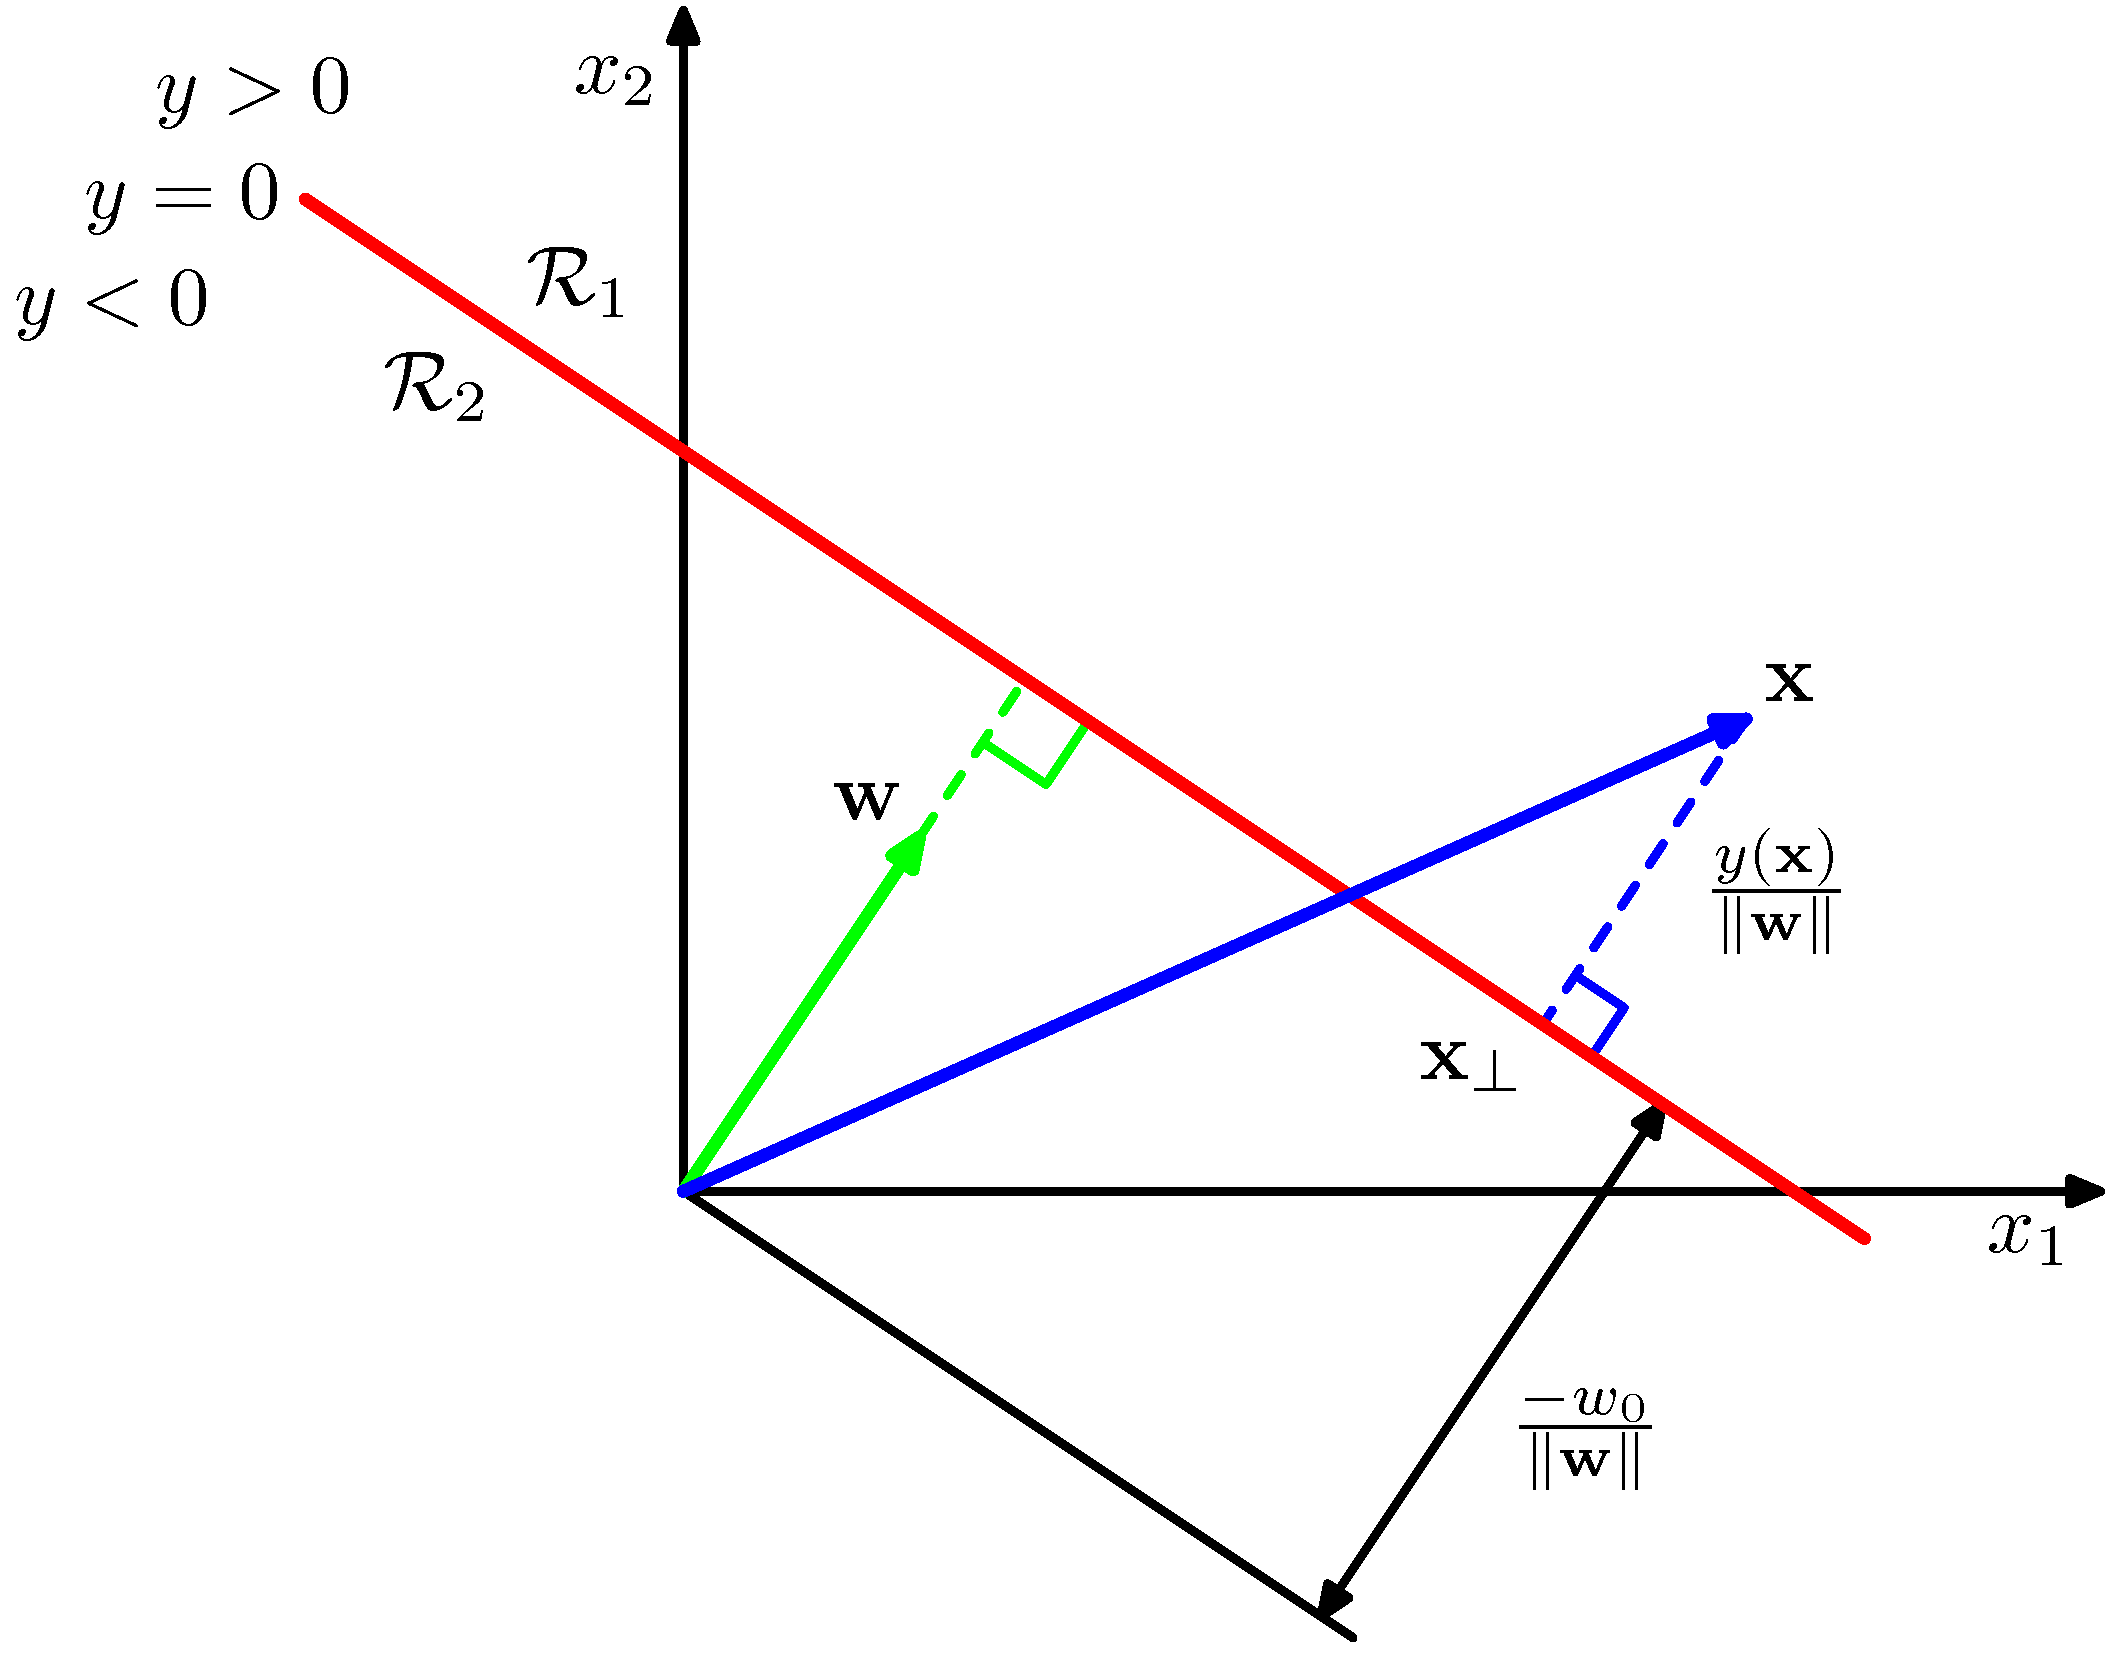
\includegraphics[scale=0.8]{Images/4-1.png}
		\captionsetup{font={small}}
		\caption{二维空间中线性判别函数的几何表示。红线为决策平面(这里也可以说成是决策边界),可以看出它是与$\bw$垂直的;决策平面相对原点的偏移量由偏差参数$w_0$控制。此外,对于一个一般的点$\bx$,它到决策平面的正交距离为$y(\bx)/\|\bw\|$。}
		\label{fig:4-1}
	\end{figure}
	\\
	\indent 另外还需要注意到,$y(\bx)$的值给出了点$\bx$到决策平面的垂直距离$r$,而且是带有符号的。为了验证这一点,设对于一个一般的点$\bx$,令$\bx_\bot$为$\bx$在决策平面上的正交投影,于是
	\begin{equation}
		\bx = \bx_\bot + r \frac{\bw}{\|\bw\|}
	\end{equation}
	在等式两侧同时乘以$\bw^{\rmT}$并加上$w_0$,根据$y(\bx)=\bw^{\rmT}\bx+w_0$和$y(\bx_\bot)=\bw^{\rmT}\bx_\bot + w_0 = 0$,可以得到
	\begin{equation}
		r = \frac{y(\bx)}{\|\bw\|}
	\end{equation}
	这一结果如图4.1所示。\\
	\indent 和第3章中研究线性回归模型时一样,有时利用另一种比较紧凑的表示方法要更方便一些,也就是加上额外的输入$x_0 = 1$从而定义$\widetilde{\bw} = (w_0,\bw)$和$\widetilde{\bx} = (x_0, \bx)$,于是
	\begin{equation}
		y(\bx) = \widetilde{\bw}^{\rmT} \widetilde{\bx}
	\end{equation}
	在这种情况下,决策平面就变成了$D+1$维的增广输入空间中的$D$维超平面,而且是必经过原点的。
	}
	\subsection{多分类问题}
	\textnormal{
	现在我们开始研究$K>2$情况下的线性判别函数。比较直观的想法是,通过将一系列二分类的判别函数结合起来形成一个$K$分类的判别函数,不过我们马上会发现这样的做法会导致一系列的麻烦(Duda and Hart, 1973)。\\
	\indent 假设现在有$K-1$个分类器,每个分类器都是针对二分类问题设计的,也就是说,每个分类器都只能判定某个点是否属于类别$\mathcal{C}_k$,即"一对其余"(one-versus-rest, OvR)分类器。图4.2中的左图展示的是3个类别的情况,可以看出多个OvR分类器结合的方法会使输入空间的划分存在无法判定的模糊区域。\\
	\indent 另外有一种替代的方法,即使用$K(K-1)/2$个二分类判别函数,每个判别函数有且仅有两个可能的类别输出,即"一对一"(one-versus-one, OvO)【译者注:翻译到这里我已经昆0v0了】分类器。然后根据判别函数的多数投票对每个点进行分类。然而,这样的做法也会遇到模糊区域的问题,如图4.2中的右图所示。
	\begin{figure}[ht]
		\begin{minipage}[t]{0.5\linewidth}
		\centering
		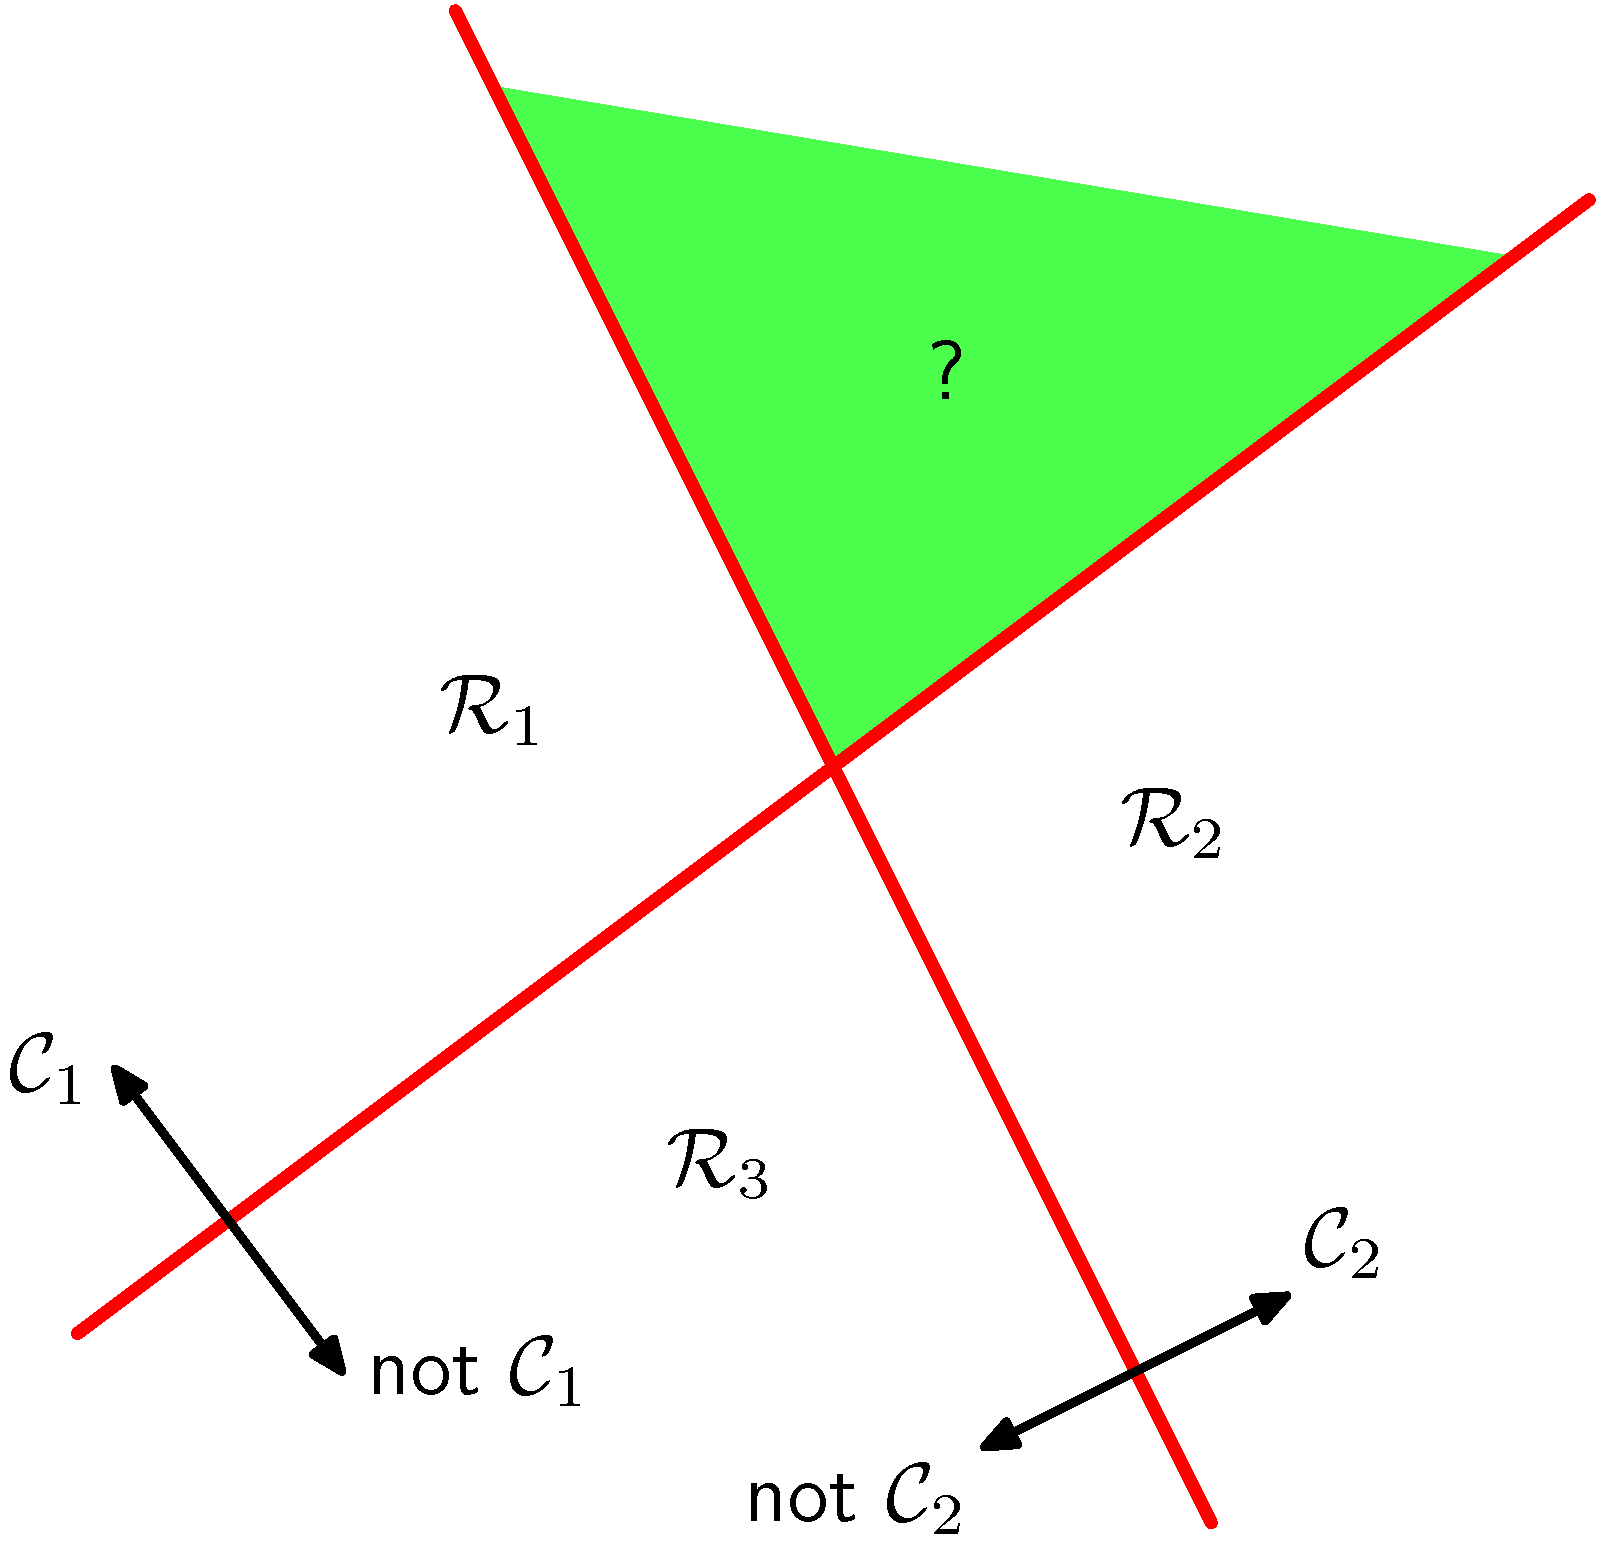
\includegraphics[scale=0.8]{Images/4-2a.png}
		\label{fig:4-2a}
		\end{minipage}
		\begin{minipage}[t]{0.5\linewidth}
		\centering
		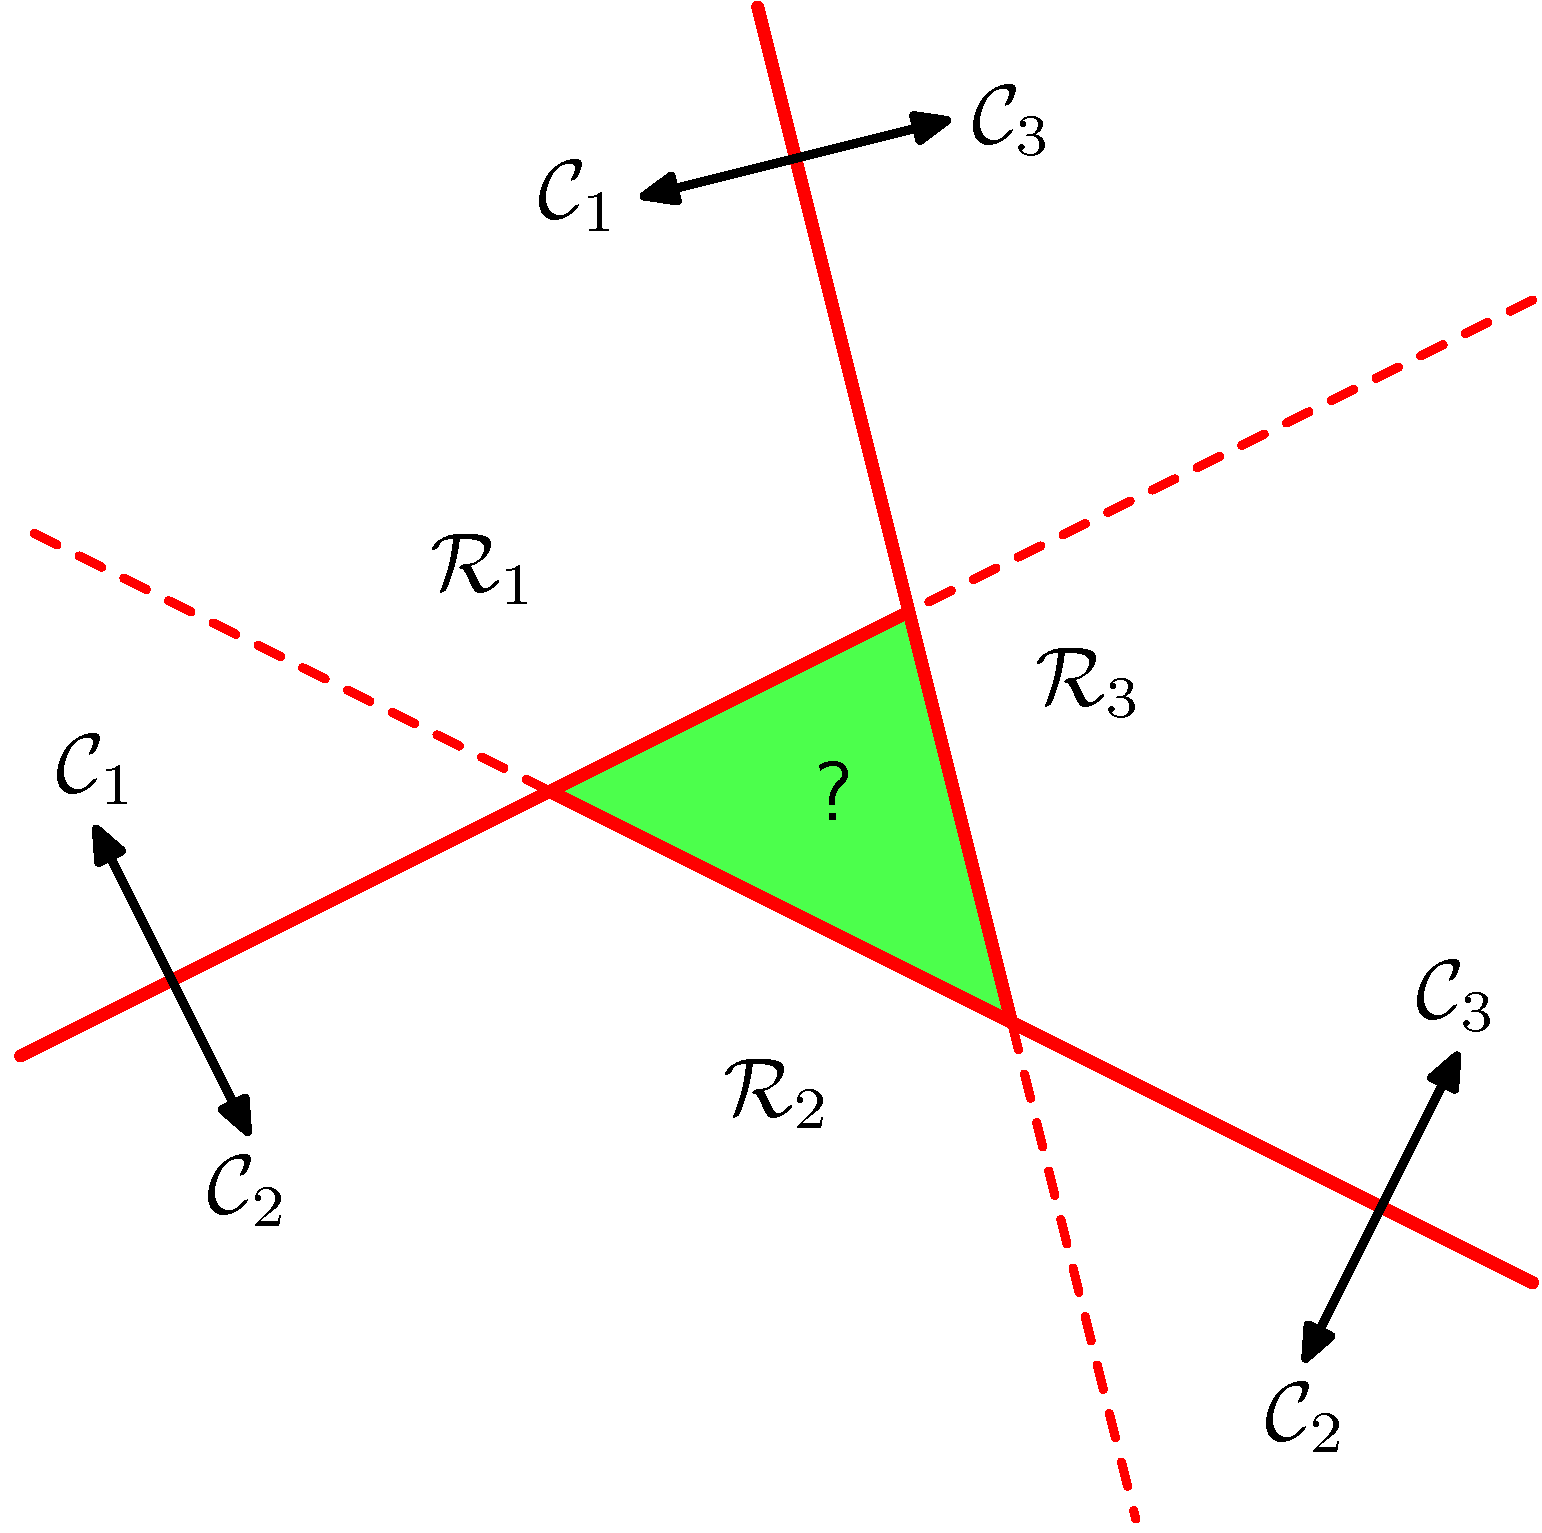
\includegraphics[scale=0.8]{Images/4-2b.png}
		\label{fig:4-2b}
		\end{minipage}
		\captionsetup{font={small}}
		\caption{通过一系列二分类判别函数建立$K$分类模型的做法会导致模糊区域的问题,如图中绿色区域所示。左图为使用OvR分类器时的情况,右图为OvO分类器时的情况。}
	\end{figure}
	\\
	\indent 不过这个问题是可以解决的。建立一个包含$K$个线性函数的$K$分类判别函数:
	\begin{equation}
		y_k(\bx) = \bw_k^{\rmT} \bx + w_{k0}
	\end{equation}
	这样一来,如果对于一切$j \neq k$都有$y_k(\bx)>y_j(\bx)$,那么$\bx$的类别就会被划分为$\mathcal{C}_k$,而且类别$\mathcal{C}_k$和$\mathcal{C}_j$之间的决策边界就是$y_k(\bx) = y_j(\bx)$,即$(D-1)$维的超平面:
	\begin{equation}
		(\bw_k - \bw_j)^{\rmT} \bx + (w_{k0} - w_{j0}) = 0
	\end{equation}
	这与第4.1.1节中二分类问题的决策边界形式相同,而且具有相同的几何性质。\\
	\indent 这样的判别函数决策域通常是单连接的,而且通常是凸的。为了验证这一点,如图4.3所示,假设决策域$\calR_k$中存在两个点$\bx_{\mathrm{A}}$和$\bx_{\mathrm{B}}$,对于一切位于$\bx_{\mathrm{A}}$和$\bx_{\mathrm{B}}$连线上的点$\hat{\bx}$都可以表示为
	\begin{equation}
		\hat{\bx} = \lambda \bx_{\mathrm{A}}+(1-\lambda)\bx_{\mathrm{B}}
	\end{equation}
	其中$0 \leqslant \lambda \leqslant 1$。根据判别函数,
	\begin{equation}
		y_k(\hat{\bx}) = \lambda y_k(\bx_{\mathrm{A}}) + (1-\lambda)y_k(\bx_{\mathrm{B}})
	\end{equation}
	由于$\bx_{\mathrm{A}}$和$\bx_{\mathrm{B}}$都位于决策域$\calR_k$内,所以对于一切$j \neq k$,一定有$y_k(\bx_{\mathrm{A}}) > y_j(\bx_{\mathrm{A}})$,以及$y_k(\bx_{\mathrm{B}}) > y_j(\bx_{\mathrm{B}})$,所以$y_k(\hat{\bx})>y_j(\hat{\bx})$,所以$\hat{\bx}$同样位于决策域$\calR_k$中。于是决策域$\calR_k$一定是单连接且凸的。
	\begin{figure}[ht]
		\centering
		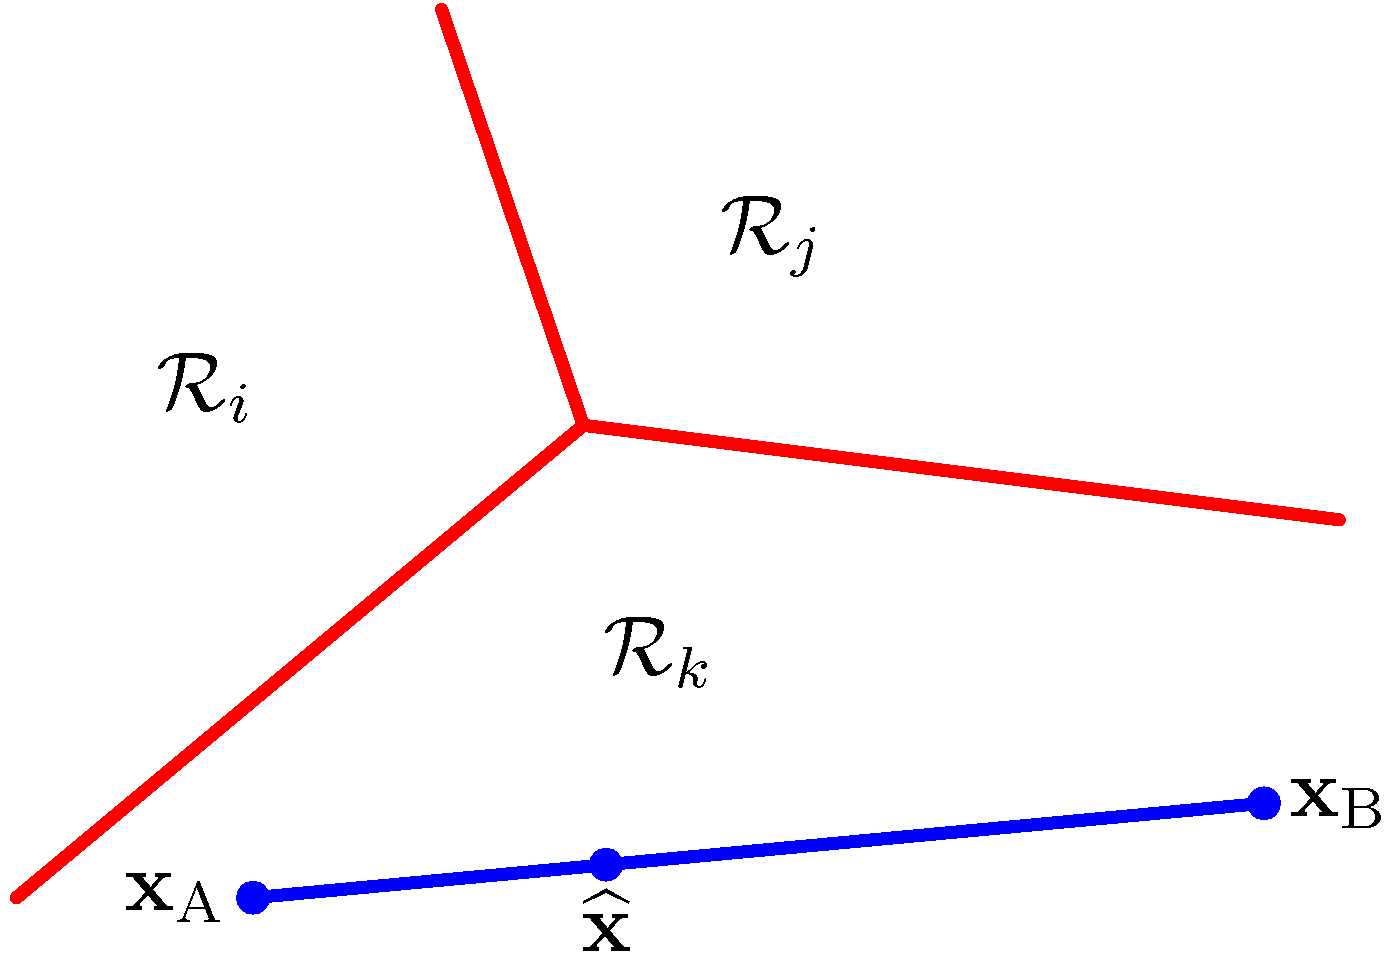
\includegraphics[scale=0.8]{Images/4-3.png}
		\captionsetup{font={small}}
		\caption{多分类问题中的线性判别决策域示意图,其中红色表示决策边界。如果两个点$\bx_{\mathrm{A}}$和$\bx_{\mathrm{B}}$都位于决策域$\calR_k$内,那么其连线上的任意点$\hat{\bx}$都一定位于$\calR_k$内,所以决策域一定是单连接且凸的。}
		\label{fig:4-3}
	\end{figure}
	\\
	\indent 对于二分类问题,我们同样可以使用这样的方法,即针对两个判别函数$y_1(\bx)$和$y_2(\bx)$或者仅使用一个第4.1.1节中更加简单但等效的判别函数$y(\bx)$进行类似的讨论。\\
	\indent 接下来我们会研究3种可以确定线性判别函数中参数的方法,分别是最小二乘法、Fisher线性判别分析和感知机算法。
	}
	\subsection{分类问题的最小二乘法}
	\textnormal{在第3章中,我们研究了参数的线性函数形式的模型,并发现通过对平方和误差函数求取最小化可以得到参数值的闭式解。所以我们自然而然地想到,能否利用类似的方法来处理分类问题。假设对于一个一般的$K$分类问题,利用1-of-K的形式表示目标向量$\sft$。在这个条件下使用最小二乘法的理由之一是,它近似等于给定输入向量条件下的目标变量的条件期望$\mathbb{E}[\sft|\bx]$。在二进制编码下,该条件期望由向量的后验分类概率给出。不过不幸的是,这样的概率近似值通常非常差劲,这是因为线性模型灵活程度有限所导致的,有时候甚至会有近似值超过范围(0,1)的情况。\\
	\indent 任意的分类$\mathcal{C}_k$都有各自的线性模型,
	\begin{equation}
		y_k(\bx) = \bw_k^{\rmT} + w_{k0}
	\end{equation}
	其中$k=1,...,K$。于是我们可以将其整合在一起,形成一个大的向量,于是
	\begin{equation}
		\mathbf{y}(\bx)=\widetilde{\mathbf{W}}^{\rmT} \widetilde{\bx}
	\end{equation}
	其中,矩阵$\widetilde{\mathbf{W}}$的第$k$列为$(D+1)$维向量$\widetilde{\bw}_k = (w_{k0}, \bw_k^{\rmT})^{\rmT}$,$\widetilde{\bx}$则表示输入向量$(1,\bx^{\rmT})^{\rmT}$,即包含了$x_0 = 1$的向量。这一表示方法已经在第3.1节中详细介绍过。对于任意的输入向量$\bx$,将它划分到哪一类的时候输出$y_k = \widetilde{\bw}_k^{\rmT}\widetilde{\bx}$取得最大值,就将它划分到哪一类。\\
	\indent 和第3章一样,现在我们要通过平方和误差函数的最小化来确定参数矩阵$\widetilde{\mathbf{W}}$。假设训练集为$\{\bx_n, \sft_n\}, n=1,...,N$,并定义矩阵$\mathbf{T}$,其第$n$行为向量$\sft_n^{\rmT}$,以及定义矩阵$\widetilde{\mathbf{X}}$,其第$n$行为$\widetilde{\bx}_n^{\rmT}$。于是平方和误差函数为
	\begin{equation}
		E_D(\widetilde{\mathbf{W}})=\frac{1}{2}\mathrm{Tr}\left\{(\widetilde{\mathbf{X}}\widetilde{\mathbf{W}}-\mathbf{T})^{\rmT}(\widetilde{\mathbf{X}}\widetilde{\mathbf{W}}-\mathbf{T})\right\}
	\end{equation}
	对$\widetilde{\mathbf{W}}$求导并令导数为0,并稍作整理,可以得到$\widetilde{\mathbf{W}}$的解
	\begin{equation}
		\widetilde{\mathbf{W}} = (\widetilde{\mathbf{X}}^{\rmT} \widetilde{\mathbf{X}})^{-1}\widetilde{\mathbf{X}}^{\rmT} \mathbf{T} = \widetilde{\mathbf{X}}^{\dagger}\mathbf{T}
	\end{equation}
	和第3.1.1节中一样,其中$\widetilde{\mathbf{X}}^{\dagger}$表示矩阵$\widetilde{\mathbf{X}}$的伪逆。于是接下来就可以确定完整的判别函数
	\begin{equation}
		\mathbf{y}(\mathbf{x})=\widetilde{\mathbf{W}}^{\rmT}\widetilde{\bx}=\mathbf{T}^{\rmT}\left(\widetilde{\mathbf{X}}^{\dagger}\right)^{\rmT}\widetilde{\bx}
	\end{equation}
	\indent 多目标变量的最小二乘解有一个有趣的性质,如果训练集中的每个目标向量都满足某参数为$\mathbf{a}$和$b$的线性约束
	\begin{equation}
		\mathbf{a}^{\rmT}\sft_n + b = 0
	\end{equation}
	那么模型对任意$\bx$产生的预测也将同样满足这一约束,即
	\begin{equation}
		\mathbf{a}^{\rmT}\mathbf{y}(\bx) + b = 0
	\end{equation}
	所以如果使用1-of-K编码的形式表示分类,那么模型所做出的预测一定满足一条性质——$\mathbf{y}(\bx)$的所有元素之和为1。不过,这一约束还不足以使得模型输出可以视为概率,因为并没有将元素约束在区间$(0,1)$内。\\
	\indent 最小二乘法确实可以求出判别函数参数的闭式解。不过,这样得到的判别函数是直接进行预测,并未考虑任何概率层面上的解释,在应用时会存在很多问题。从图4.4可以看出,最小二乘解缺乏针对异常值的鲁棒性,这一问题同样会出现在分类问题中。其中,右侧图中所示的附加数据点对决策边界产生了严重的影响,更可恨的是,要是像左图中那样进行划分,这些点还是可以被正确分类的。平方和误差函数会对远离决策边界,但处于正确区域的"过于正确"的预测进行惩罚。在第7.1.2节中,我们会研究若干种分类问题中其他类型的误差函数,而且会发现它们就不会遇到这样的麻烦。
	\begin{figure}[H]
		\begin{minipage}[t]{0.5\linewidth}
		\centering
		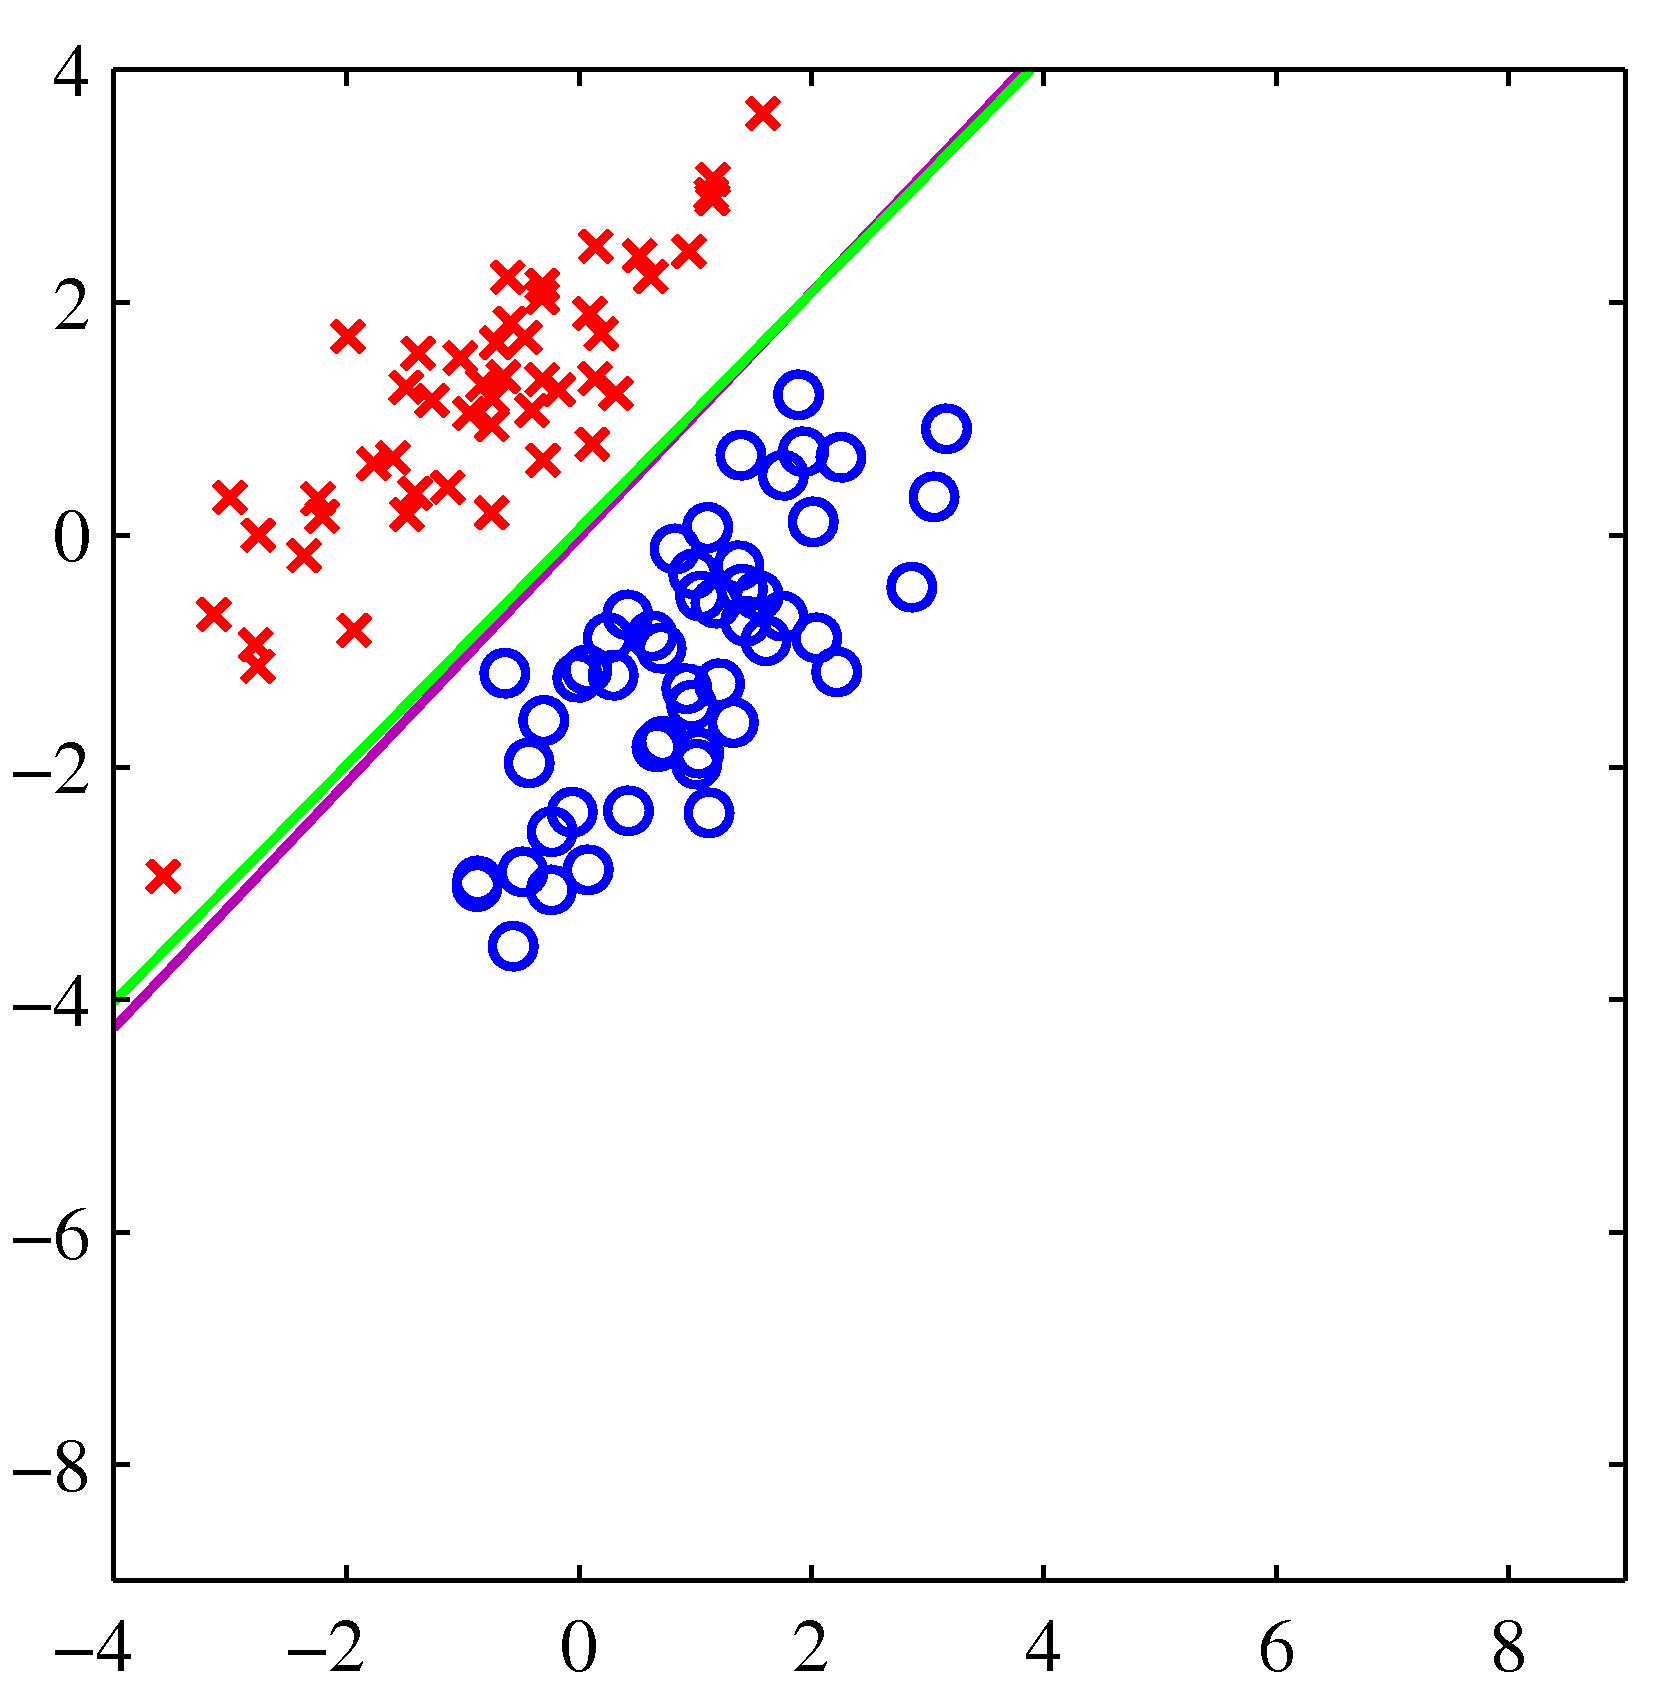
\includegraphics[scale=0.8]{Images/4-4a.png}
		\label{fig:4-4a}
		\end{minipage}
		\begin{minipage}[t]{0.5\linewidth}
		\centering
		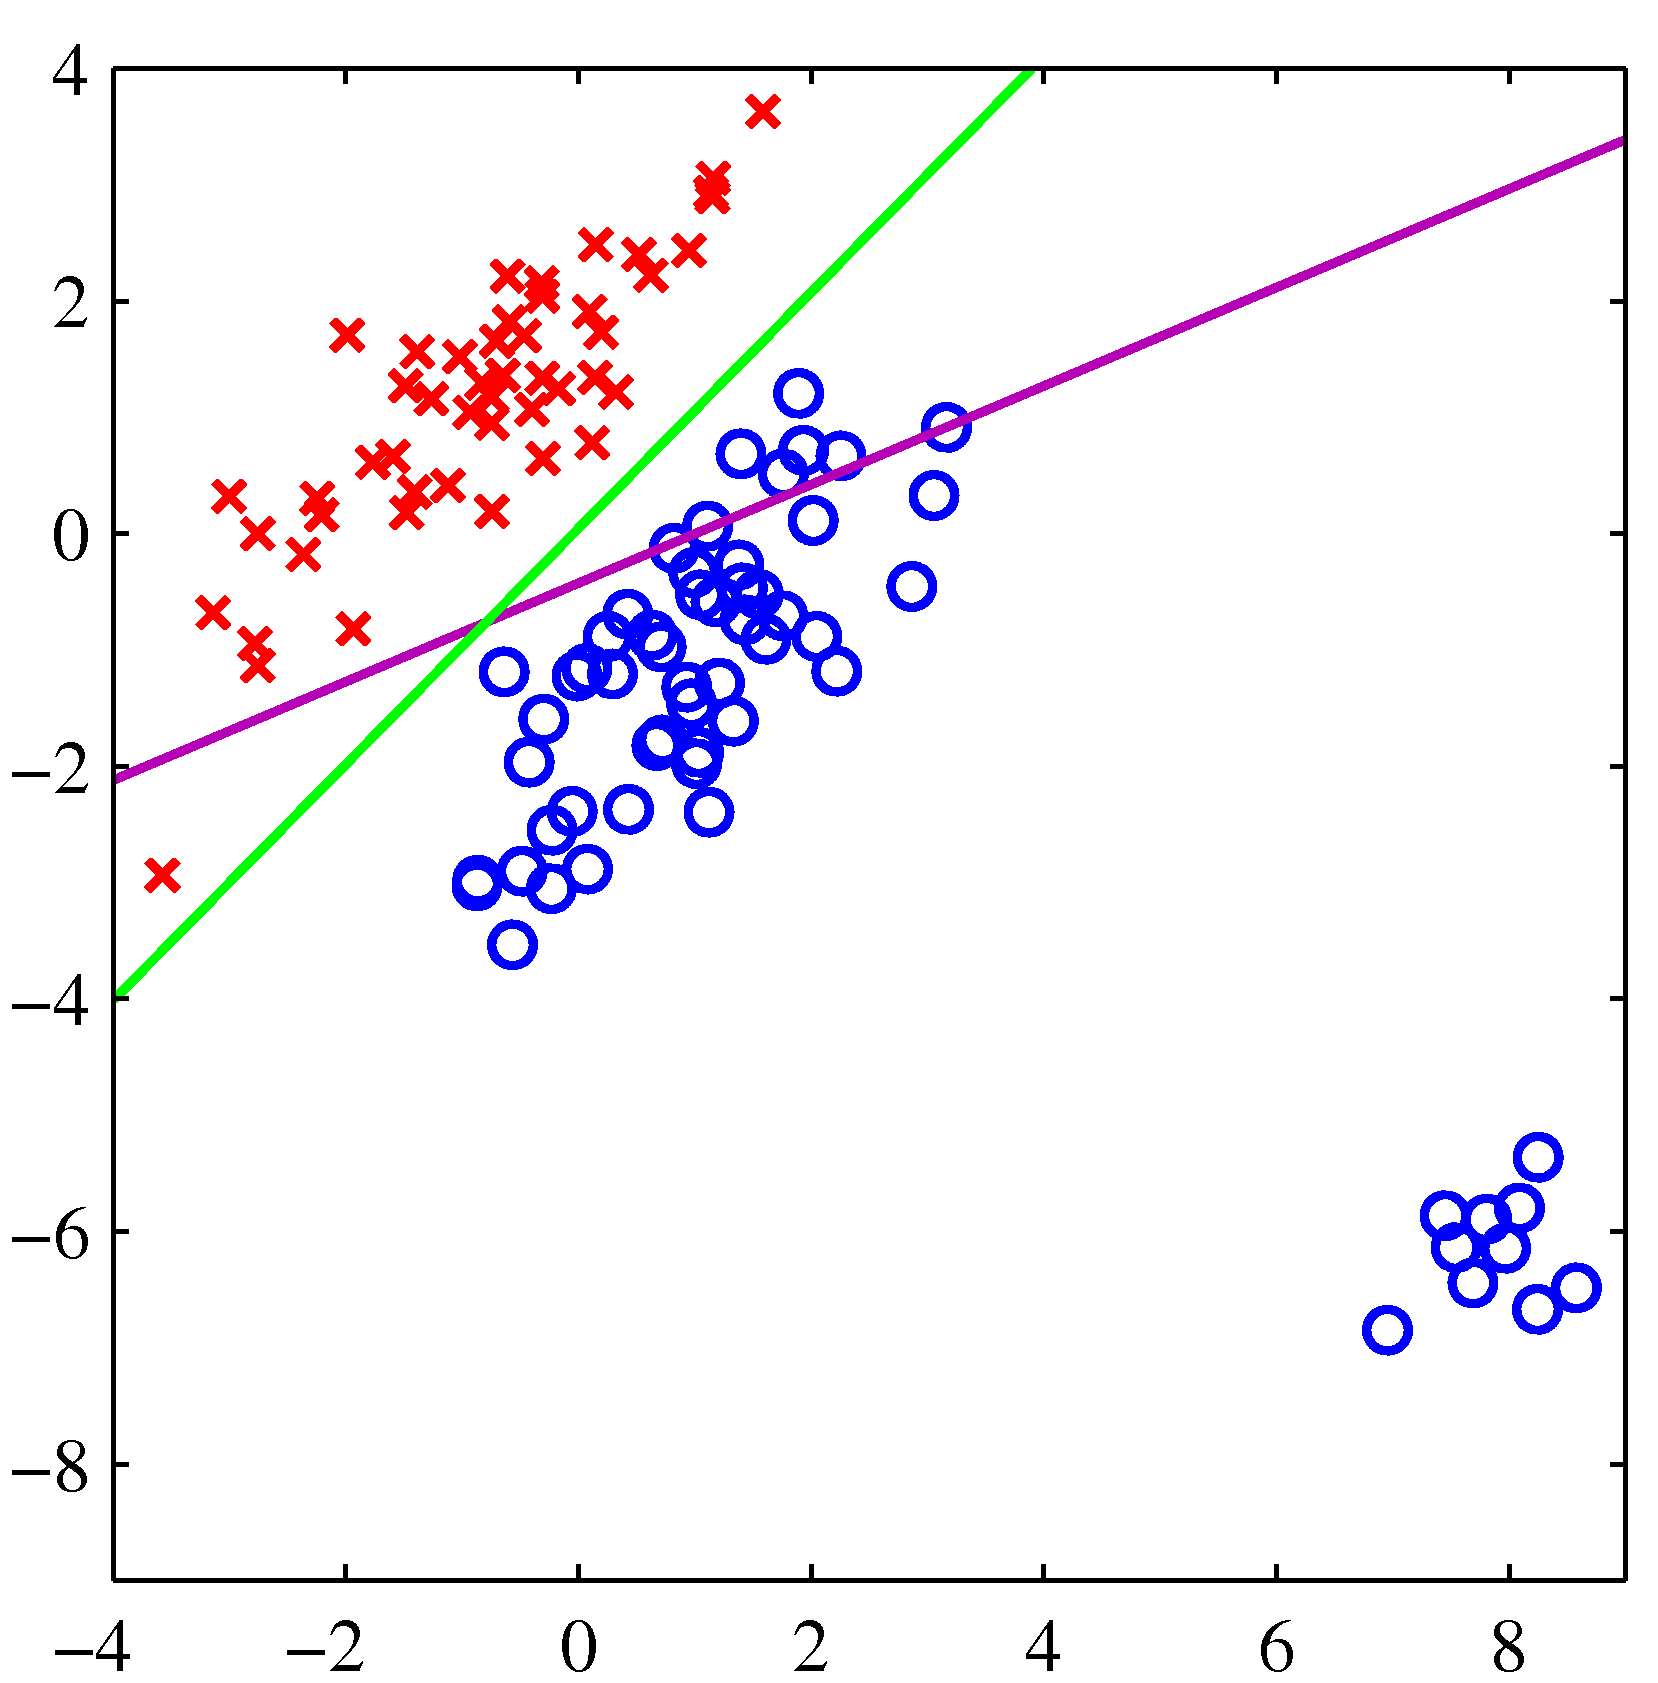
\includegraphics[scale=0.8]{Images/4-4b.png}
		\label{fig:4-4b}
		\end{minipage}
		\captionsetup{font={small}}
		\caption{左图中展示的是两类数据以及通过最小二乘法(紫红色)和logistic回归模型(绿色,即将在第4.3.2节中讨论)得到的决策边界,两类数据分别表示为个红色叉号和蓝色圆圈。右图中展示的是添加了一些附加数据后决策边界的变化情况,可以看出最小二乘法得到的决策边界对异常值过于敏感,而logistic回归方法则不会这样。}
		\begin{minipage}[t]{0.5\linewidth}
		\centering
		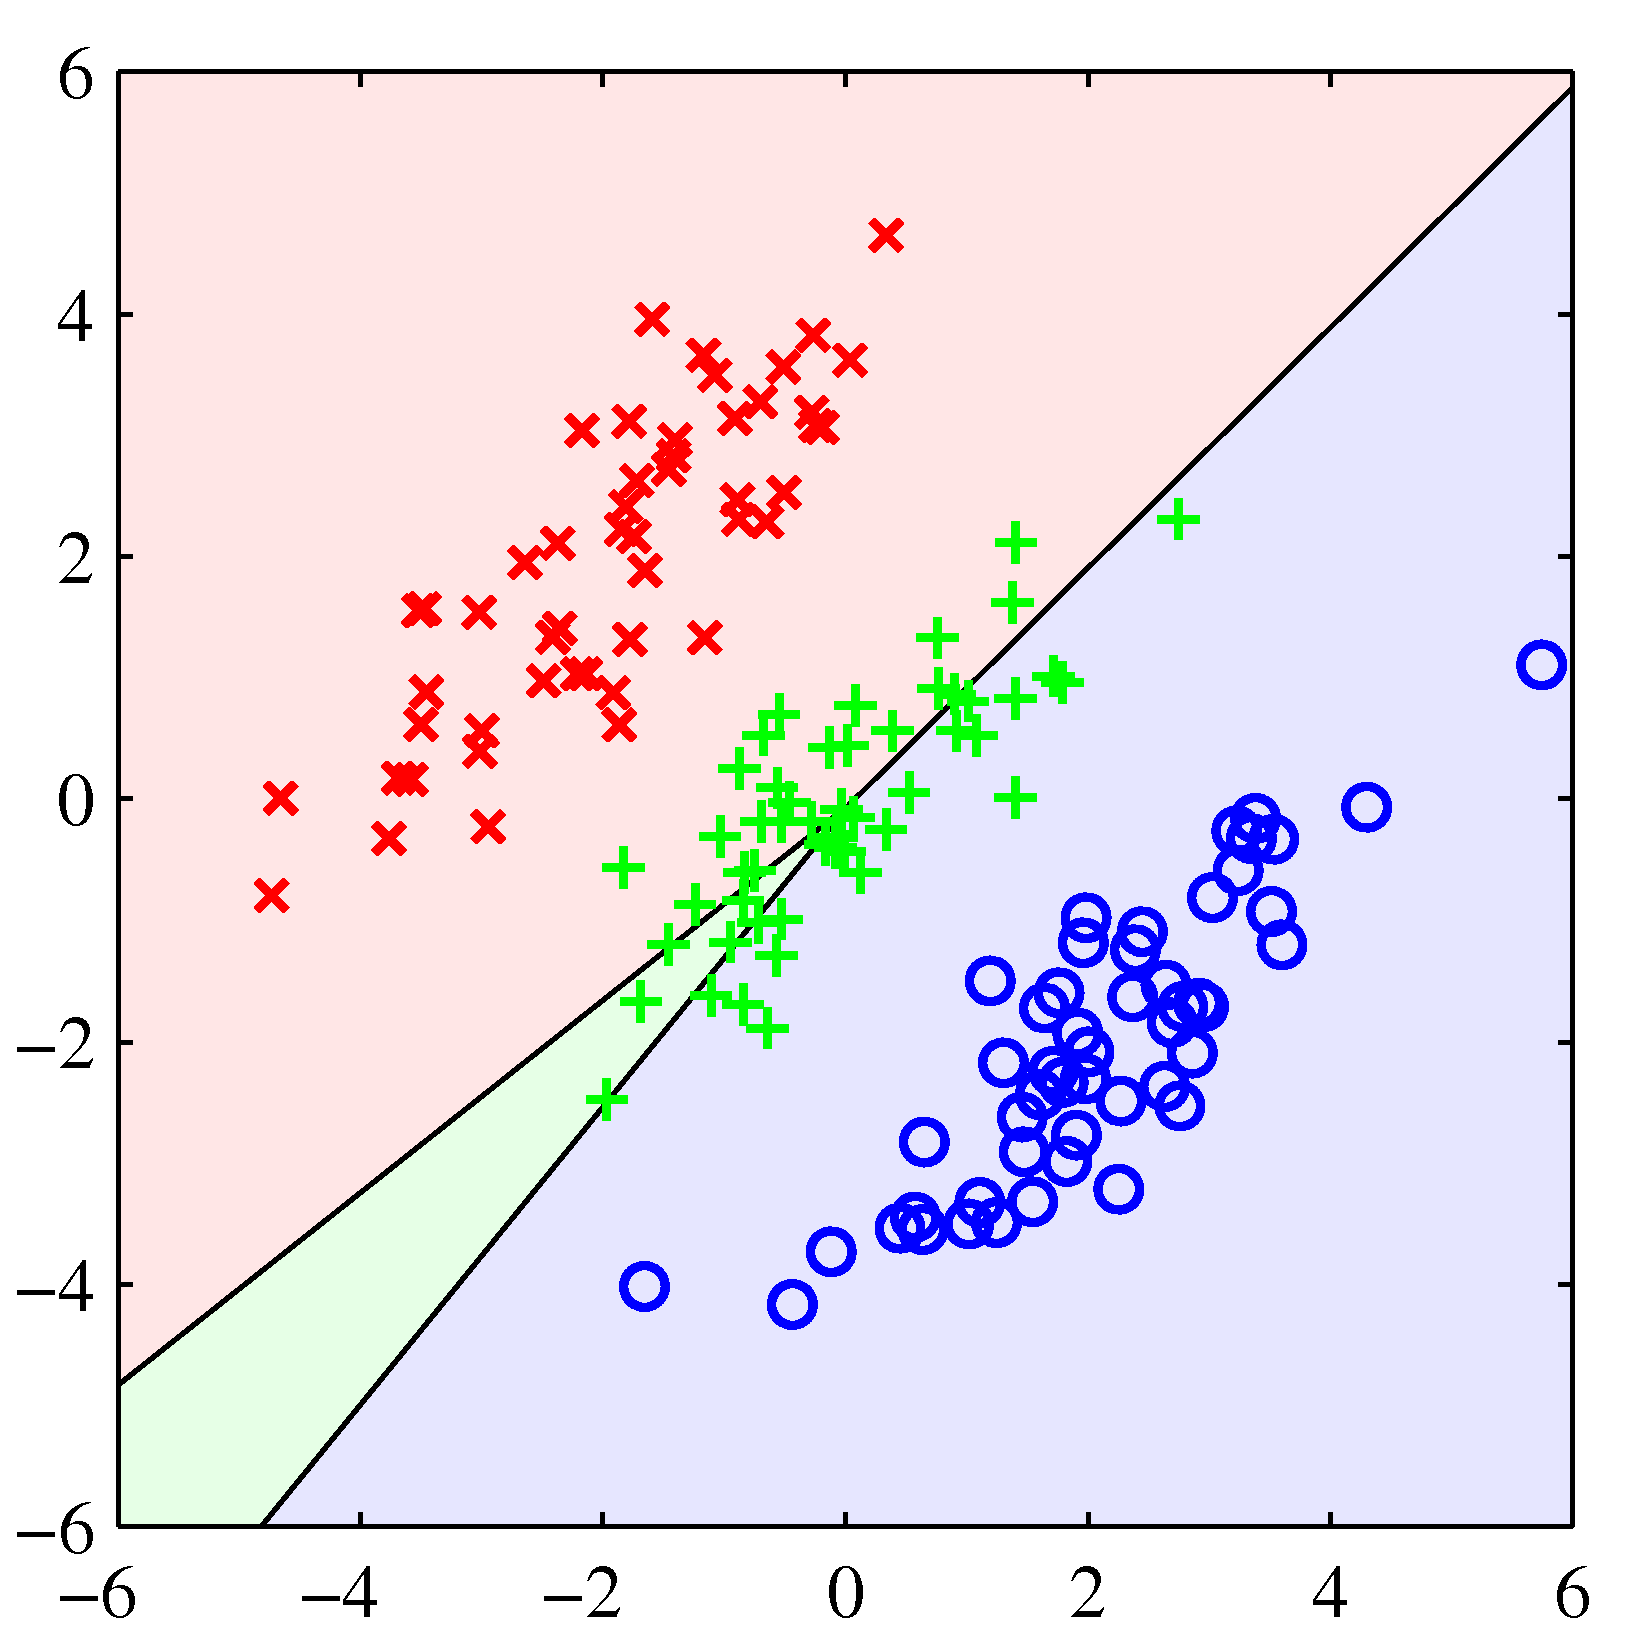
\includegraphics[scale=0.8]{Images/4-5a.png}
		\label{fig:4-5a}
		\end{minipage}
		\begin{minipage}[t]{0.5\linewidth}
		\centering
		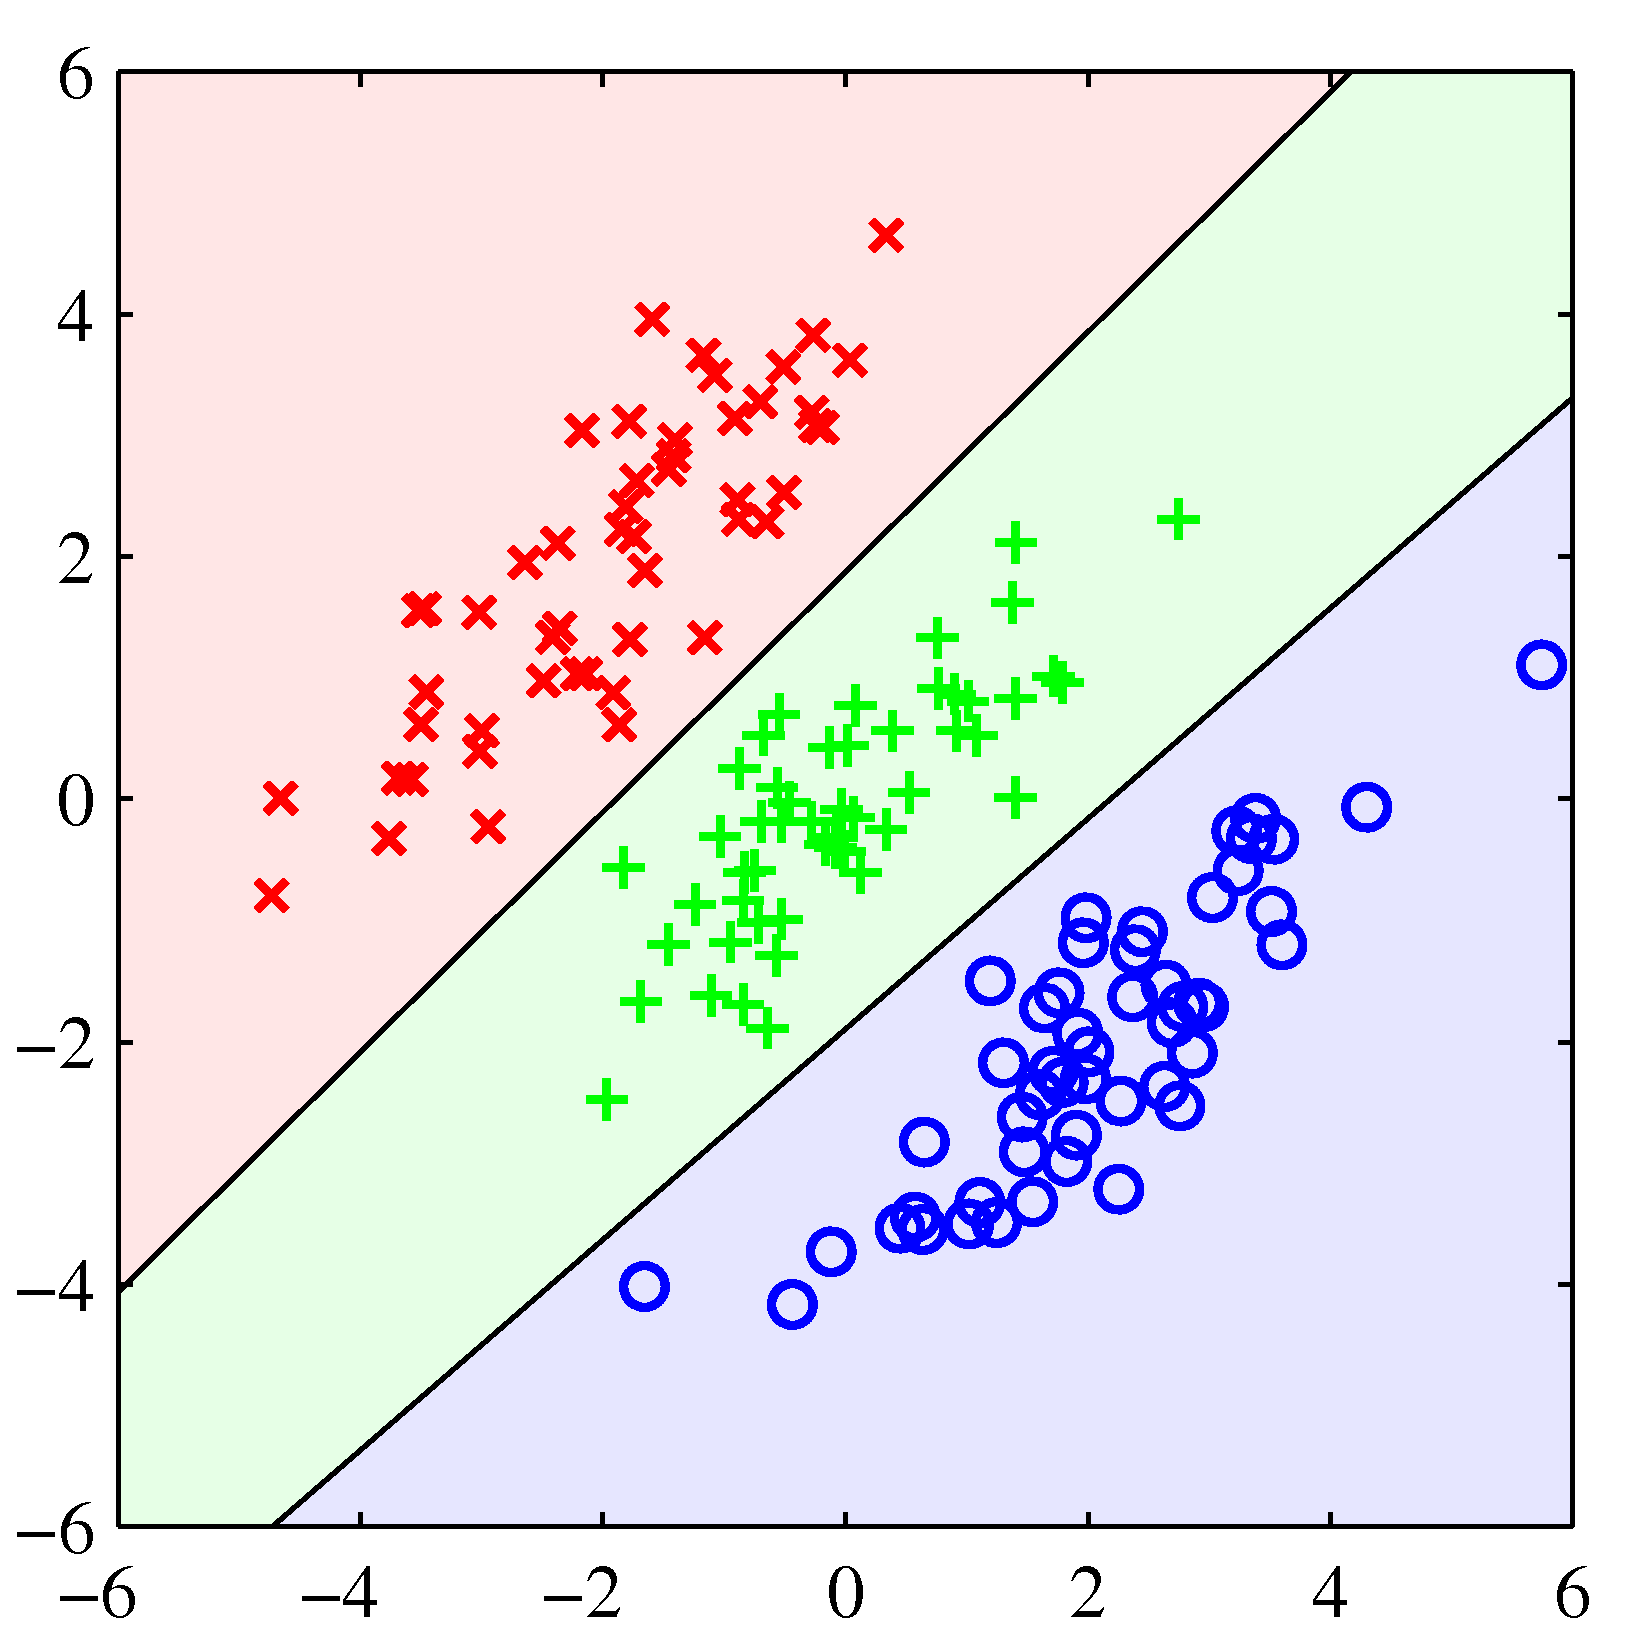
\includegraphics[scale=0.8]{Images/4-5b.png}
		\label{fig:4-5b}
		\end{minipage}
		\captionsetup{font={small}}
		\caption{对于一个包含3个类别的线性可分数据集,其中训练数据的类别分别表示为红色叉号、绿色十字和蓝色圆圈。图中的直线表示决策边界,背景颜色表示各自的决策域。左图是采用最小二乘法进行判别的结果。可以看出分给绿色类别的决策域非常小,绝大多数点都被误分类了。右图是采用第4.3.2节中即将介绍的logistic回归进行判别的结果,很明显分类的效果要好很多。}
	\end{figure}
	\indent 然而,最小二乘法存在的问题还不止于此。如图4.5所示,在二维输入空间$(x_1,x_2)$中存在一个包含3个类别的数据集,而且该数据集是线性可分的。利用本章后续即将介绍的logistic回归方法,可以得到右图那样很好的结果,但最小二乘法得到的结果却很差,输入空间只有很小的一部分划分给了绿色的类别。\\
	\indent 最小二乘法的不尽如人意其实并不令人以外,因为最小二乘法事实上对应的是高斯条件分布假设下的最大似然,但二元的目标向量的分布很明显与高斯分布差了十万八千里。采用更加合适的概率模型,可以得到比最小二乘法效果更好的分类方法。不过现在我们先继续研究确定线性分类模型参数的非概率方法。
	}
	\subsection{Fisher线性判别分析}
	\textnormal{从降维的视角看待线性分类模型的一种不错的方法。首先研究二分类问题,假设输入向量$\bx$的维度为$D$,经过如下的投影:
	\begin{equation}
		y = \bw^{\rmT}\bx
	\end{equation}
	可以将其变为一维,假如存在某个关于$y$的阈值,如果$y \geqslant -w_0$则分类为$\mathcal{C}_1$,否则分类为$\mathcal{C}_2$,这样一来就得到了前面所讨论的线性分类器。一般而言,将向量投影到一维空间中不可避免地会造成信息的损失,而且在原始的$D$维空间中所划分的类别会在一维空间中存在严重的重叠。不过,通过调整权重向量$\bw$,我们可以选择一个使得类别分离度最大化的投影方式。首先,假设在二分类问题中有$N_1$个点属于类别$\mathcal{C}_1$,$N_2$个点属于类别$\mathcal{C}_2$,那么两个类别各自的均值向量分别为
	\begin{equation}
		\mathbf{m}_1 = \frac{1}{N_1}\sum_{n \in \mathcal{C}_1} \bx_n, \mathbf{m}_2 = \frac{1}{N_2}\sum_{n \in \mathcal{C}_2}\bx_n
	\end{equation}
	当投影到$\bw$上时类别均值的投影是类别分离度最简单的衡量标准。也就是说我们应当选择使得
	\begin{equation}
		m_2 - m_1 = \bw^{\rmT}(\mathbf{m}_2 - \mathbf{m}_1)
	\end{equation}
	取得最大值的$\bw$,其中
	\begin{equation}
		m_k = \bw^{\rmT}\mathbf{m}_k
	\end{equation}
	为类别$\mathcal{C}_k$的数据投影后的均值。不过这里有个毛病,随便增加$\bw$的大小,就可以使$m_k$变成任意大小。为了解决这个问题,我们可以给$\bw$加上单位化的限定,即$\sum_i w_i^2 = 1$。利用拉格朗日乘数法构建约束优化问题,可以得出一个结论——$\bw \propto (\mathbf{m}_2 - \mathbf{m}_1)$。
	\begin{figure}[ht]
		\begin{minipage}[t]{0.5\linewidth}
		\centering
		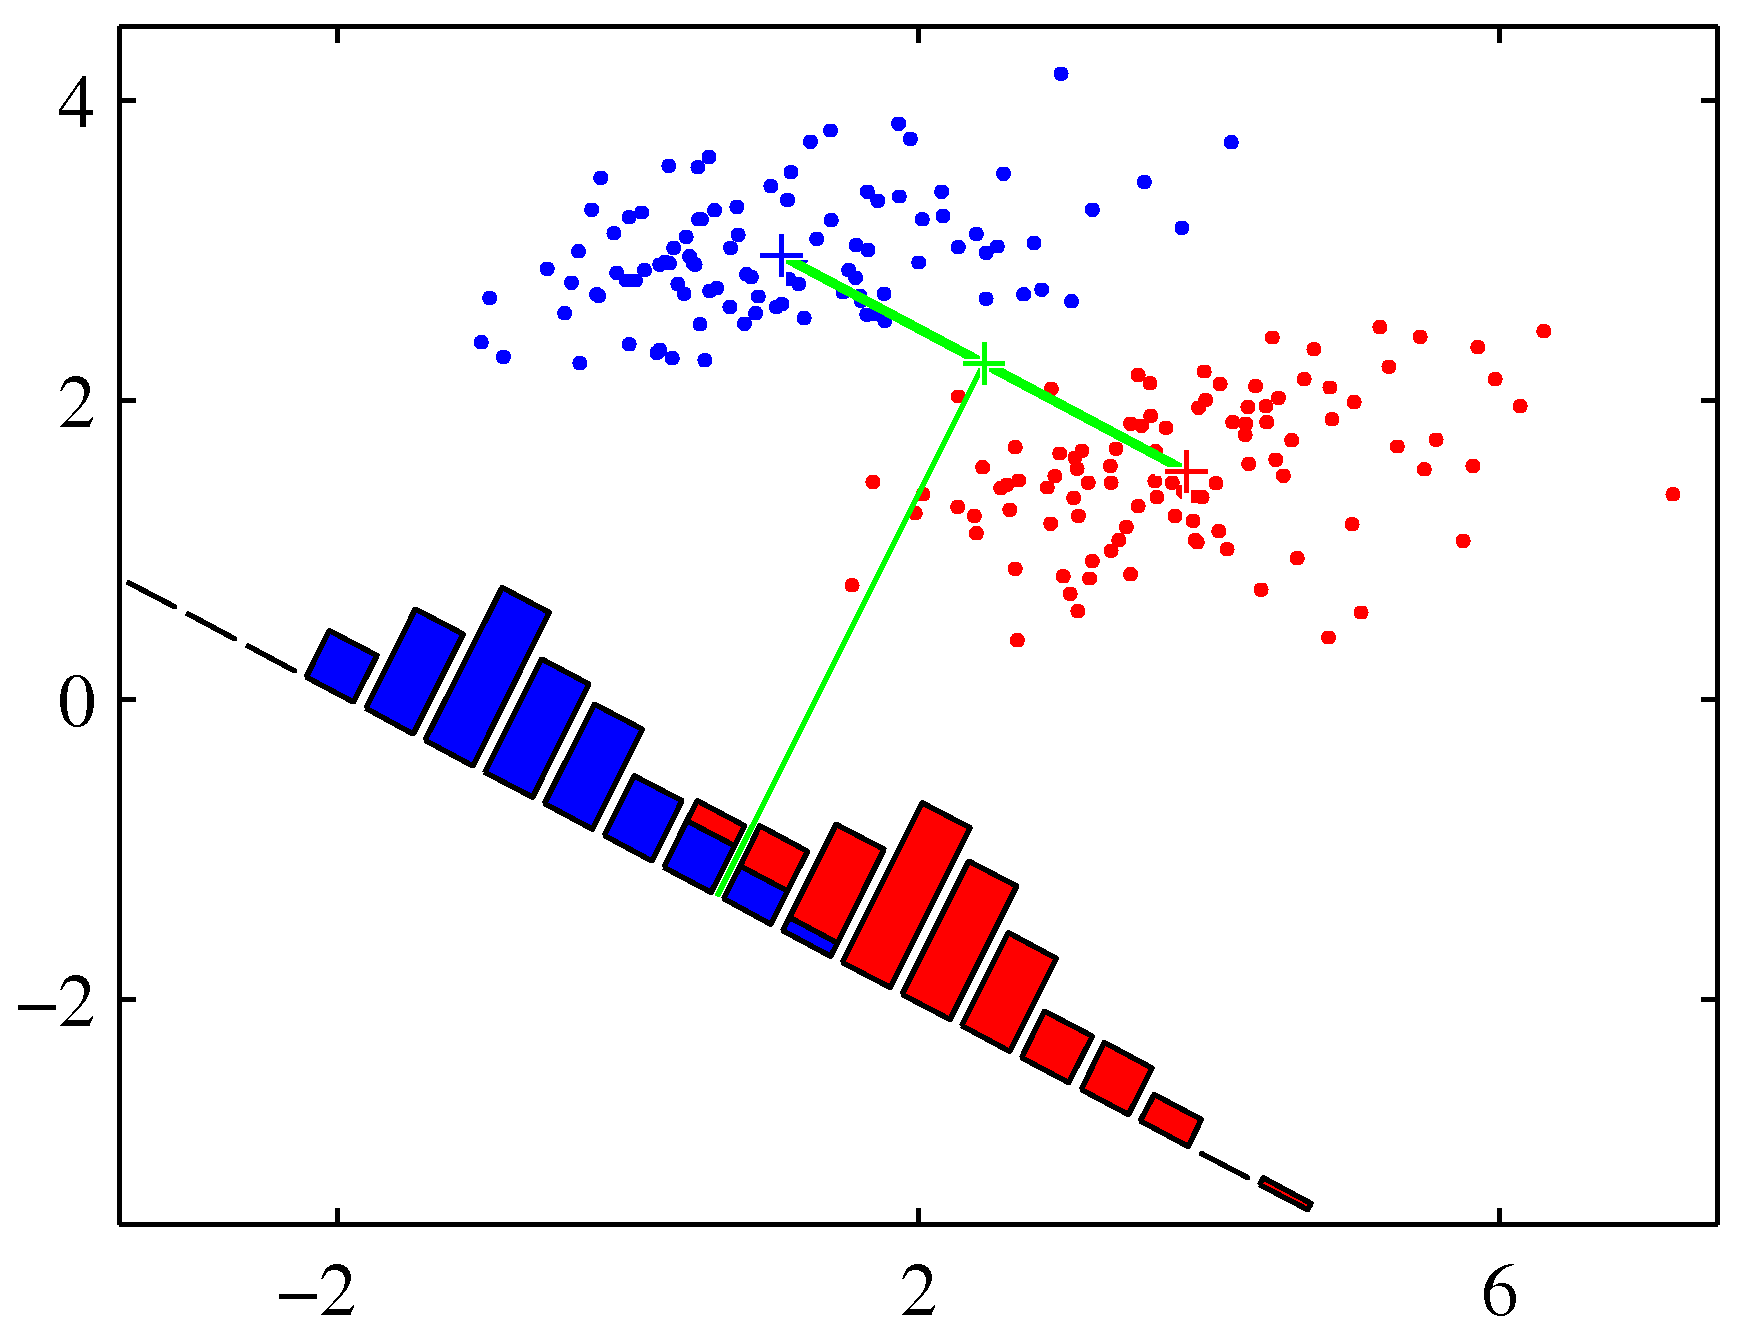
\includegraphics[scale=0.8]{Images/4-6a.png}
		\label{fig:4-6a}
		\end{minipage}
		\begin{minipage}[t]{0.5\linewidth}
		\centering
		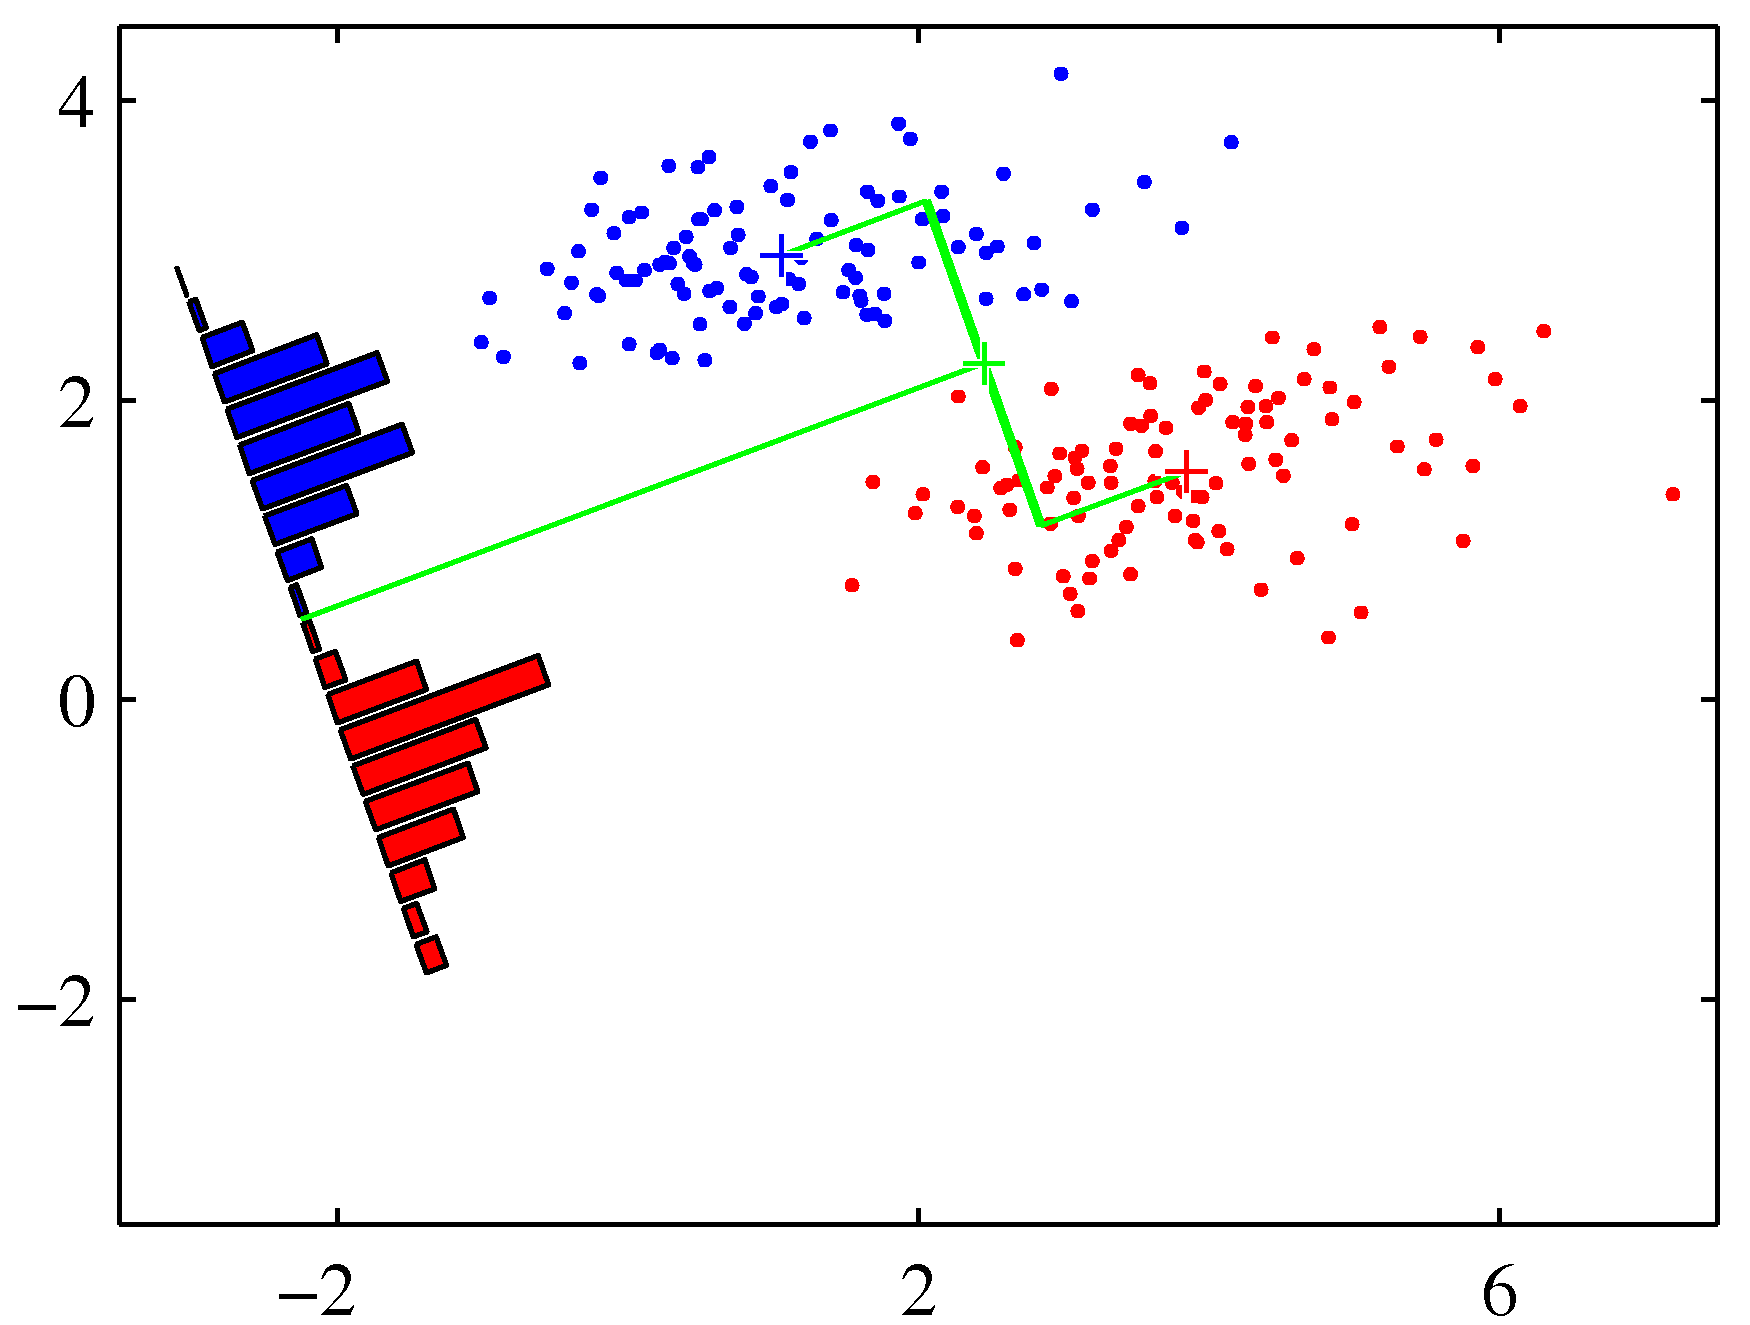
\includegraphics[scale=0.8]{Images/4-6b.png}
		\label{fig:4-6b}
		\end{minipage}
		\captionsetup{font={small}}
		\caption{左图中展示的是两类数据(红色和蓝色)投影到两类数据各自均值的连线上之后的直方图。需要注意的是,其中出现了类别重叠的问题。右图中展示的是基于Fisher线性判别分析的投影结果,很明显具有更好的效果。}
	\end{figure}
	\\
	\indent 不过这个方法还是有个问题,如图4.6所示。假设在二维输入空间$(x_1,x_2)$中存在线性可分的两类数据,但在投影到两类数据均值的连线上之后出现了严重的重叠现象。当类别的概率分布的协方差矩阵与对角矩阵相差较大时就会出现这样的问题。Fisher提出的方法是对某个函数进行最大化,这个函数可以使得投影后的类别均值分离度较大,同时使每个类别内的方差较小,从而使类别重叠最小化。\\
	\indent 投影公式(4.20)可以将一系列的$\bx$投影到一维空间$y$中。每个类别$\mathcal{C}_k$内的数据经过变换后,其方差为
	\begin{equation}
		s_k^2 = \sum_{n \in \mathcal{C}_k}(y_n - m_k)^2
	\end{equation}
	其中$y_n = \bw^{\rmT} \bx_n$。在整个数据集上,所有类别内方差的总和可以定义为$s_1^2 + s_2^2$。Fisher的方法就是定义了类别间方差与类别内方差的比值,即
	\begin{equation}
		J(\bw)=\frac{(m_2-m_1)^2}{s_1^2 + s_2^2}
	\end{equation}
	利用(4.20),(4.23)和(4.24),将以上公式改写为
	\begin{equation}
		J(\bw)=\frac{\bw^{\rmT}\mathbf{S}_\mathrm{B}\bw}{\bw^{\rmT}\mathbf{S}_\mathrm{W}\bw}
	\end{equation}
	其中$\mathbf{S}_\mathrm{B}$为类别间的协方差矩阵,
	\begin{equation}
		\mathbf{S}_\mathrm{B} = (\mathbf{m}_2 - \mathbf{m}_1)(\mathbf{m}_2 - \mathbf{m}_1)^{\rmT}
	\end{equation}
	$\mathbf{S}_\mathrm{W}$为类别内协方差矩阵的总和,
	\begin{equation}
		\mathbf{S}_\mathrm{W}=\sum_{n \in \mathcal{C}_1}(\bx_n - \mathbf{m}_1)(\bx_n - \mathbf{m}_1)^{\rmT} + \sum_{n \in \mathcal{C}_2}(\bx_n - \mathbf{m}_2)(\bx_n - \mathbf{m}_2)^{\rmT}
	\end{equation}
	对(4.26)关于$\bw$求导,可以得出当
	\begin{equation}
		(\bw^{\rmT}\mathbf{S}_\mathrm{B}\bw)\mathbf{S}_\mathrm{W}\bw = (\bw^{\rmT}\mathbf{S}_\mathrm{W}\bw)\mathbf{S}_\mathrm{B}\bw
	\end{equation}
	时,$J(\bw)$取得最大值。根据(4.27),可以看出$\mathbf{S}_\mathrm{B}\bw$始终处于$(\mathbf{m}_2 - \mathbf{m}_1)$方向上。另外,我们不太关心$\bw$的大小,而是只关心它的方向,所以尺度因子$\bw^{\rmT}\mathbf{S}_\mathrm{B}\bw$和$\bw^{\rmT}\mathbf{S}_\mathrm{W}\bw$可以直接扔掉不管。在(4.29)等式两侧同时乘以$\mathbf{S}_\mathrm{W}^{-1}$,
	\begin{equation}
		\bw \propto \mathbf{S}_\mathrm{W}^{-1}(\mathbf{m}_2 - \mathbf{m}_1)
	\end{equation}
	需要注意的是,如果类别内协方差是各项同性的,那么$\mathbf{S}_\mathrm{W}$将是单位矩阵的倍数,而$\bw$与类别之间的差距成正比。\\
	\indent 公式(4.30)就是Fisher线性判别公式。不过严格来说,它更像是数据投影到一维空间时的方向选择,而非判别函数。然而,经过投影的数据接下来就可以构建判别函数了,只需设置一个阈值$y_0$,当$y(\bx)\geqslant y_0$时分类为$\mathcal{C}_1$,否则分类为$\mathcal{C}_2$。举例而言,我们可以利用高斯分布对类别条件概率密度$p(y|\mathcal{C}_k)$进行建模,然后利用第1.2.4节中的最大似然方法求取高斯分布的参数。得到投影类别的近似高斯分布后,可以利用第1.5.1节中的方法求出最优的阈值。由于$y=\bw^{\rmT}\bx$是一系列随机变量的和,所以可以利用中心极限定理对高斯分布进行一些假设。
	}
	\subsection{与最小二乘法的关系}
	\textnormal{
	用于确定线性判别函数的最小二乘法建立在一个原则之上,那就是让目标变量的预测尽可能地接近真实值。相比之下,Fisher方法则是要尽可能在输出空间使类别的分离度达到最大。这两种方法之间的关系也比较有意思。特别地,对于二分类问题,Fisher方法事实上是最小二乘法的一种特殊情况。\\
	\indent 到目前为止我们一直在用1-of-K编码来表示目标变量。不过,如果我们换一种目标变量的表示方式,那么权重向量的最小二乘解将等价于Fisher方法的解(Duda and Hart, 1973)。特别地,令属于类别$\mathcal{C}_1$的目标值为$N/N_1$,其中$N_1$为类别$\mathcal{C}_1$中的模式数量,$N$为模式总数。这个目标值近似等于类别$\mathcal{C}_1$的先验概率的倒数。对于类别$\mathcal{C}_2$,可以令目标值为$-N/N_2$,其中$N_2$为类别$\mathcal{C}_2$中的模式数量。\\
	\indent 平方和误差函数可以写成
	\begin{equation}
		E = \frac{1}{2}\sum_{n=1}^N (\bw^{\rmT}\bx_n + w_0 -t_n)^2
	\end{equation}
	分别令$E$关于$w_0$和$\bw$的导数等于0,可以得到
	\begin{align}
		\sum_{n=1}^N(\bw^{\rmT}\bx_n + w_0 - t_n)&=0\\
		\sum_{n=1}^N(\bw^{\rmT}\bx_n + w_0 -t_n)\bx_n &= 0
	\end{align}
	根据(4.32)和目标变量$t_n$的表示方法,可以确定偏差的表达式
	\begin{equation}
		w_0 = -\bw^{\rmT}\mathbf{m}
	\end{equation}
	其中用到了一个结果,
	\begin{equation}
		\sum_{n=1}^N t_n =N_1\frac{N}{N_1} - N_2\frac{N}{N_2} = 0
	\end{equation}
	以及$\mathbf{m}$是整个数据集上的均值,其表达式为
	\begin{equation}
		\mathbf{m} = \frac{1}{N}\sum_{n=1}^N \bx_n = \frac{1}{N}(N_1 \mathbf{m}_1 + N_2\mathbf{m}_2)
	\end{equation}
	经过一系列计算之后,(4.33)会演变成
	\begin{equation}
		\left(\mathbf{S}_\mathrm{W} + \frac{N_1 N_2}{N}\mathbf{S}_\mathrm{B}\right)\bw = N(\mathbf{m}_1 - \mathbf{m}_2)
	\end{equation}
	其中$\mathbf{S}_\mathrm{W}$定义于(4.28),$\mathbf{S}_\mathrm{B}$定义于(4.27),同时代入了偏差(4.34)。根据(4.27),$\mathbf{S}_\mathrm{B}\bw$始终处于$(\mathbf{m}_2 - \mathbf{m}_1)$的方向上。所以
	\begin{equation}
		\bw \propto \mathbf{S}_\mathrm{W}^{-1}(\mathbf{m}_2 - \mathbf{m}_1)
	\end{equation}
	其中忽略了无关的尺度因子。由此可见,权重向量恰好与Fisher方法所得到的结果相同。此外(4.34)给出了偏差$w_0$的值。这个结论告诉我们,对于一个新的向量$\bx$,如果$y(\bx) = \bw^{\rmT}(\bx - \mathbf{m})>0$,那么它应该分类到类别$\mathcal{C}_1$中,否则应当分类为$\mathcal{C}_2$。
	}
	\subsection{多分类问题中的Fisher线性判别分析}
	\textnormal{现在我们研究Fisher线性判别分析推广到$K>2$的多分类问题中的情况,假设输入空间的维度$D$大于类别的数量$K$。然后,我们引入$D'>1$个线性“特征”$y_k = \bw_k^{\rmT}\bx$,其中$k=1,...,D'$。这次特征的值可以整合成一个独立的向量$\mathbf{y}$。类似地,权重向量$\left\{\bw_k\right\}$可以看成是矩阵$\mathbf{W}$的列,于是
	\begin{equation}
		\mathbf{y} = \mathbf{W}^{\rmT}\bx
	\end{equation}
	需要注意的是,在$\mathbf{y}$的定义中没有出现偏差参数。根据(4.28),$K$分类问题的类别内协方差矩阵为
	\begin{equation}
		\mathbf{S}_\mathrm{W} = \sum_{k=1}^K \mathbf{S}_k
	\end{equation}
	其中
	\begin{align}
		\mathbf{S}_k &= \sum_{n \in \mathcal{C}_k}(\bx_n - \mathbf{m}_k)(\bx_n - \mathbf{m}_k)^{\rmT} \\
		\mathbf{m}_k &= \frac{1}{N_k}\sum_{n \in \mathcal{C}_k}\bx_n
	\end{align}
	$N_k$表示类别$\mathcal{C}_k$中的数据数量。为了求出类别间协方差矩阵,根据Duda and Hart(1973),首先求出协方差矩阵总和
	\begin{equation}
		\mathbf{S}_\mathrm{T} = \sum_{n=1}^N(\bx_n - \mathbf{m}_k)(\bx_n - \mathbf{m}_k)^{\rmT}
	\end{equation}
	其中$\mathbf{m}$表示整个数据集的均值
	\begin{equation}
		\mathbf{m} = \frac{1}{N} \sum_{n=1}^N\bx_n = \frac{1}{N}\sum_{k=1}^K N_k\mathbf{m}_k
	\end{equation}
	$N = \sum_k N_k$表示数据总数。协方差矩阵的总和可以拆分为类别内协方差矩阵的总和(4.40)与类别间协方差矩阵$\mathbf{S}_\mathrm{B}$(4.41)的和,也就是说
	\begin{equation}
		\mathbf{S}_\mathrm{T} = \mathbf{S}_\mathrm{W} + \mathbf{S}_\mathrm{B}
	\end{equation}
	其中
	\begin{equation}
		\mathbf{S}_\mathrm{B} = \sum_{k=1}^K N_k (\mathbf{m}_k - \mathbf{m})(\mathbf{m}_k - \mathbf{m})^{\rmT}
	\end{equation}
	这些协方差矩阵都是定义在原始$\bx$空间内的。现在可以定义投影到$D'$维$\mathbf{y}$空间内的类似的矩阵:
	\begin{align}
		\mathbf{S}_\mathrm{W} &= \sum_{k=1}^K \sum_{n \in \mathcal{C}_k}(\mathbf{y}_n - \bfMu_k)(\mathbf{y}_n - \bfMu_k)^{\rmT}\\
		\mathbf{S}_\mathrm{B} &= \sum_{k=1}^K N_k(\bfMu_k - \bfMu)(\bfMu_k - \bfMu)^{\rmT}
	\end{align}
	其中
	\begin{equation}
		\bfMu_k = \frac{1}{N_k}\sum_{n \in \mathcal{C}_k}\mathbf{y}_n, \bfMu = \frac{1}{N}\sum_{k=1}^K N_k \bfMu_k
	\end{equation}
	和之前一样,我们希望建立一个在类别间协方差很大的情况下类别内协方差很小的判定标准。这有很多种选择(Fukunaga, 1990),比如
	\begin{equation}
		J(\mathbf{W})=\mathrm{Tr}\left\{\mathbf{S}_\mathrm{W}^{-1} \mathbf{S}_\mathrm{B}\right\}
	\end{equation}
	这个等式可以写成投影矩阵函数的形式
	\begin{equation}
		J(\mathbf{W}) = \mathrm{Tr}\left\{(\mathbf{W}^{\rmT}\mathbf{S}_{\mathrm{W}}\mathbf{W})^{-1}(\mathbf{W}^{\rmT}\mathbf{S}_\mathrm{B}\mathbf{W})\right\}
	\end{equation}
	对这个函数进行最大化是很直接的,在Fukunaga(1990)中有详细的讨论。权重的值则是矩阵$\mathbf{S}_{\mathrm{W}}^{\rmT} \mathbf{S}_\mathrm{B}$最大特征值所对应的特征向量。\\
	\indent 对于所有的评价标准来说,有一件事是统一的。首先通过(4.46)发现$\mathbf{S}_\mathrm{B}$是由$K$个矩阵求和得到的,而且每个矩阵都是两个向量的外积,所以这个矩阵的秩一定为1。此外,根据(4.44)的约束,只有$(K-1)$个矩阵是相互独立的。所以,$\mathbf{S}_\mathrm{B}$的秩其实至多为$(K-1)$,也就是说,至多有$(K-1)$个非零特征值。所以,$\mathbf{S}_\mathrm{B}$的特征向量在$(K-1)$维子空间中的投影跨度并不影响$J(\mathbf{W})$的值,以及我们不可能找到$(K-1)$以上个线性“特征”(Fukunaga, 1990)。
	}
	\subsection{感知机算法}
	\textnormal{线性判别模型的另一个重要案例是Rosenblatt在1962年提出的感知机算法。它解决的是二分类问题,首先要将输入向量$\bx$进行非线性变换,从而得到新的向量$\phi(\bx)$,然后构建广义线性模型
	\begin{equation}
		y(\bx) = f\left(\bw^{\rmT}\phi(\bx)\right)
	\end{equation}
	其中的非线性激活函数$f(\cdot)$为阶跃函数,
	\begin{equation}
		f(a) = \left\{ \begin{matrix} 
			+1, a \geqslant 0 \\
			-1, a < 0
		\end{matrix}\right.
	\end{equation}
	向量$\phi(\bx)$中包含有偏差分量$\phi_0(\bx) = 1$。在以前的一些关于二分类问题的讨论中,我们一般将目标变量的取值设置为$t \in {0,1}$,这样的做法是为了适应概率模型的需要。不过在感知机算法中,将目标变量设置为$t \in {+1, -1}$要更好一些,所以我们选择了这样的激活函数。\\
	\indent 通过误差函数最小化,可以很容易地得到感知机的参数$\bw$。对于这个误差函数,人们会很自然而然地想到将其设置为误分类数据的总数。不过,这样一来学习算法就会变得复杂,因为误差函数会成为关于$\bw$的分段常值函数,当$\bw$发生变化时,一旦决策边界发生变化,直接会导致误差函数的不连续。所以这样的话想要对$\bw$求取梯度从而对误差函数进行最小化的思路就行不通了,因为这个梯度几乎处处为零。\\
	\indent 所以我们需要换一个误差函数,这个误差函数称为感知机准则函数(perceptron criterion)。首先注意到,我们想求取的权重向量要满足这样的条件,对于属于类别$\mathcal{C}_1$的数据,要有$\bw^{\rmT}\phi(\bx_n)>0$,属于类别$\mathcal{C}_2$的数据则要有$\bw^{\rmT}\phi(\bx_n)<0$。在$t \in {-1, +1}$这样的编码规则下,我们希望让所有的数据都能够满足$\bw^{\rmT}\phi(\bx_n)t_n > 0$。在所有数据都正确分类的情况下,感知机准则函数为0,而对于误分类的$\bx_n$,感知机准则函数要使得$\bw^{\rmT}\phi(\bx_n)t_n$的值达到最小。于是,感知机准则函数为
	\begin{equation}
		E_\mathrm{P}(\bw) = -\sum_{n \in \mathcal{M}}\bw^{\rmT}\phi_n t_n
	\end{equation}
	其中$\phi_n = \phi(x_n)$,$\mathcal{M}$表示误分类集合。错误分类对该函数的造成的影响是$\bw$空间中关于$\bw$的线性函数,而正确分类对函数的影响则是0。所以误差函数是分段的线性函数。\\
	\indent 现在利用随机梯度下降法处理误差函数。权重向量$\bw$的变化情况为
	\begin{equation}
		\bw^{(\tau+1)} = \bw^{(\tau)} - \eta \nabla E_\mathrm{P}(\bw) = \bw^{(\tau)}+\eta \phi_n t_n
	\end{equation}
	其中$\eta$为学习率参数,$\tau$表示算法的迭代次数。对$\bw$乘以一个常数并不会对感知机函数$y(\bx, \bw)$造成影响,所以我们可以不失一般性地将$\eta$设置为1。需要注意的是,随着权重向量在训练中的变化,误分类样本的集合也会随之变化。\\
	\indent 感知机学习算法有一种简单的理解方式,如下所述。当我们一次又一次地遍历数据集中的数据,对于每一个$\bx_n$都计算其对应的感知机函数值(4.52)。如果这个数据的分类是正确的,那么就不修改权重向量;但如果这个数据的分类是错误的,那么对于类别$\mathcal{C}_1$我们将向量$\phi(\bx_n)$加在目前的权重向量$\bw$的估计值中,对于类别$\mathcal{C}_2$则从$\bw$中减去$\phi(\bx_n)$。感知机学习算法如图4.7所示。\\
	\indent 现在我们将目光集中到感知机学习算法过程中的一次更新上,并推导它的影响究竟是什么样的。实际上在针对这一误分类数据的更新中,这个数据分类错误的影响是在降低的,因为根据(4.55),如果将学习率设置为$\eta = 1$的话,
	\begin{equation}
		-\bw^{(\tau+1)\rmT}\phi_n t_n = -\bw^{(\tau) \rmT} \phi_n t_n - (\phi_n t_n)^{\rmT} \phi_n t_n < -\bw^{(\tau)\rmT}\phi_n t_n
	\end{equation}
	其中利用了$\|\phi_n t_n\|^2 >0$这一特性。当然,这可并不意味着其他的错误分类数据造成的误差也会降低。更要命的是,在权重向量发生更新时,此前的某些正确分类数据可能会变成错误的。因此,感知机学习算法并不能保证在每一次迭代的过程中总误差函数一定是减小的。\\
	\indent 不过,根据感知机收敛定理(perceptron convergence theorem),如果感知机算法存在精确解(或者说训练数据集是线性可分的),那么感知机算法一定可以在有限的步骤内找到这个精确解。该定理的证明可以在Rosenblatt(1962),Block(1962),Nilsson(1965),Minsky and Papert(1969),Hertz et al.(1991)和Bishop(1995a)等文献中找到。不过需要注意的是,达到收敛所需要的步数是很多的,而且在实际应用中,在实现收敛之前,我们根本没办法判定这个问题究竟是收敛速度太慢还是根本不能收敛。\\
	\indent 即使数据集是线性可分的,也可能有许多结果,具体会得到哪个结果取决于参数的初始化和数据点的出现顺序。 此外,对于线性不可分的数据集,感知器学习算法永远不会收敛。\\
	\indent 除了学习上的困难,感知机算法还有一些缺点,即没有概率输出,也不容易推广到$K>2$的分类问题。此外,最要命的限制其实是它仍然是基于固定基底函数的线性组合(是不是有点似曾相识?)。关于感知机局限性的讨论可以在Minsky and Papert(1969)和Bishop(1995a)中找到。\\
	\indent 感知器的模拟硬件实现由Rosenblatt构建,基于电机驱动的可变电阻器来实现自适应参数$w_j$。如图4.8所示。输入是从基于光传感器阵列的简单相机系统获得的,而基函数φ可以以各种方式选择,例如基于来自输入图像的随机选择的像素子集的简单固定功能。 典型应用涉及学习区分简单形状或字符。\\
	\indent 在感知器正在开发的同时,Widrow及其同事正在研究一种与之密切相关的称为“adaline”系统,该系统是“自适应线性元素”的缩写。该模型的功能形式与感知器的功能形式相同,但采用了不同的训练方法(Widrow and Hoff,1960; Widrow and Lehr,1990)。
	\begin{figure}[H]
		\begin{minipage}[t]{0.5\linewidth}
		\centering
		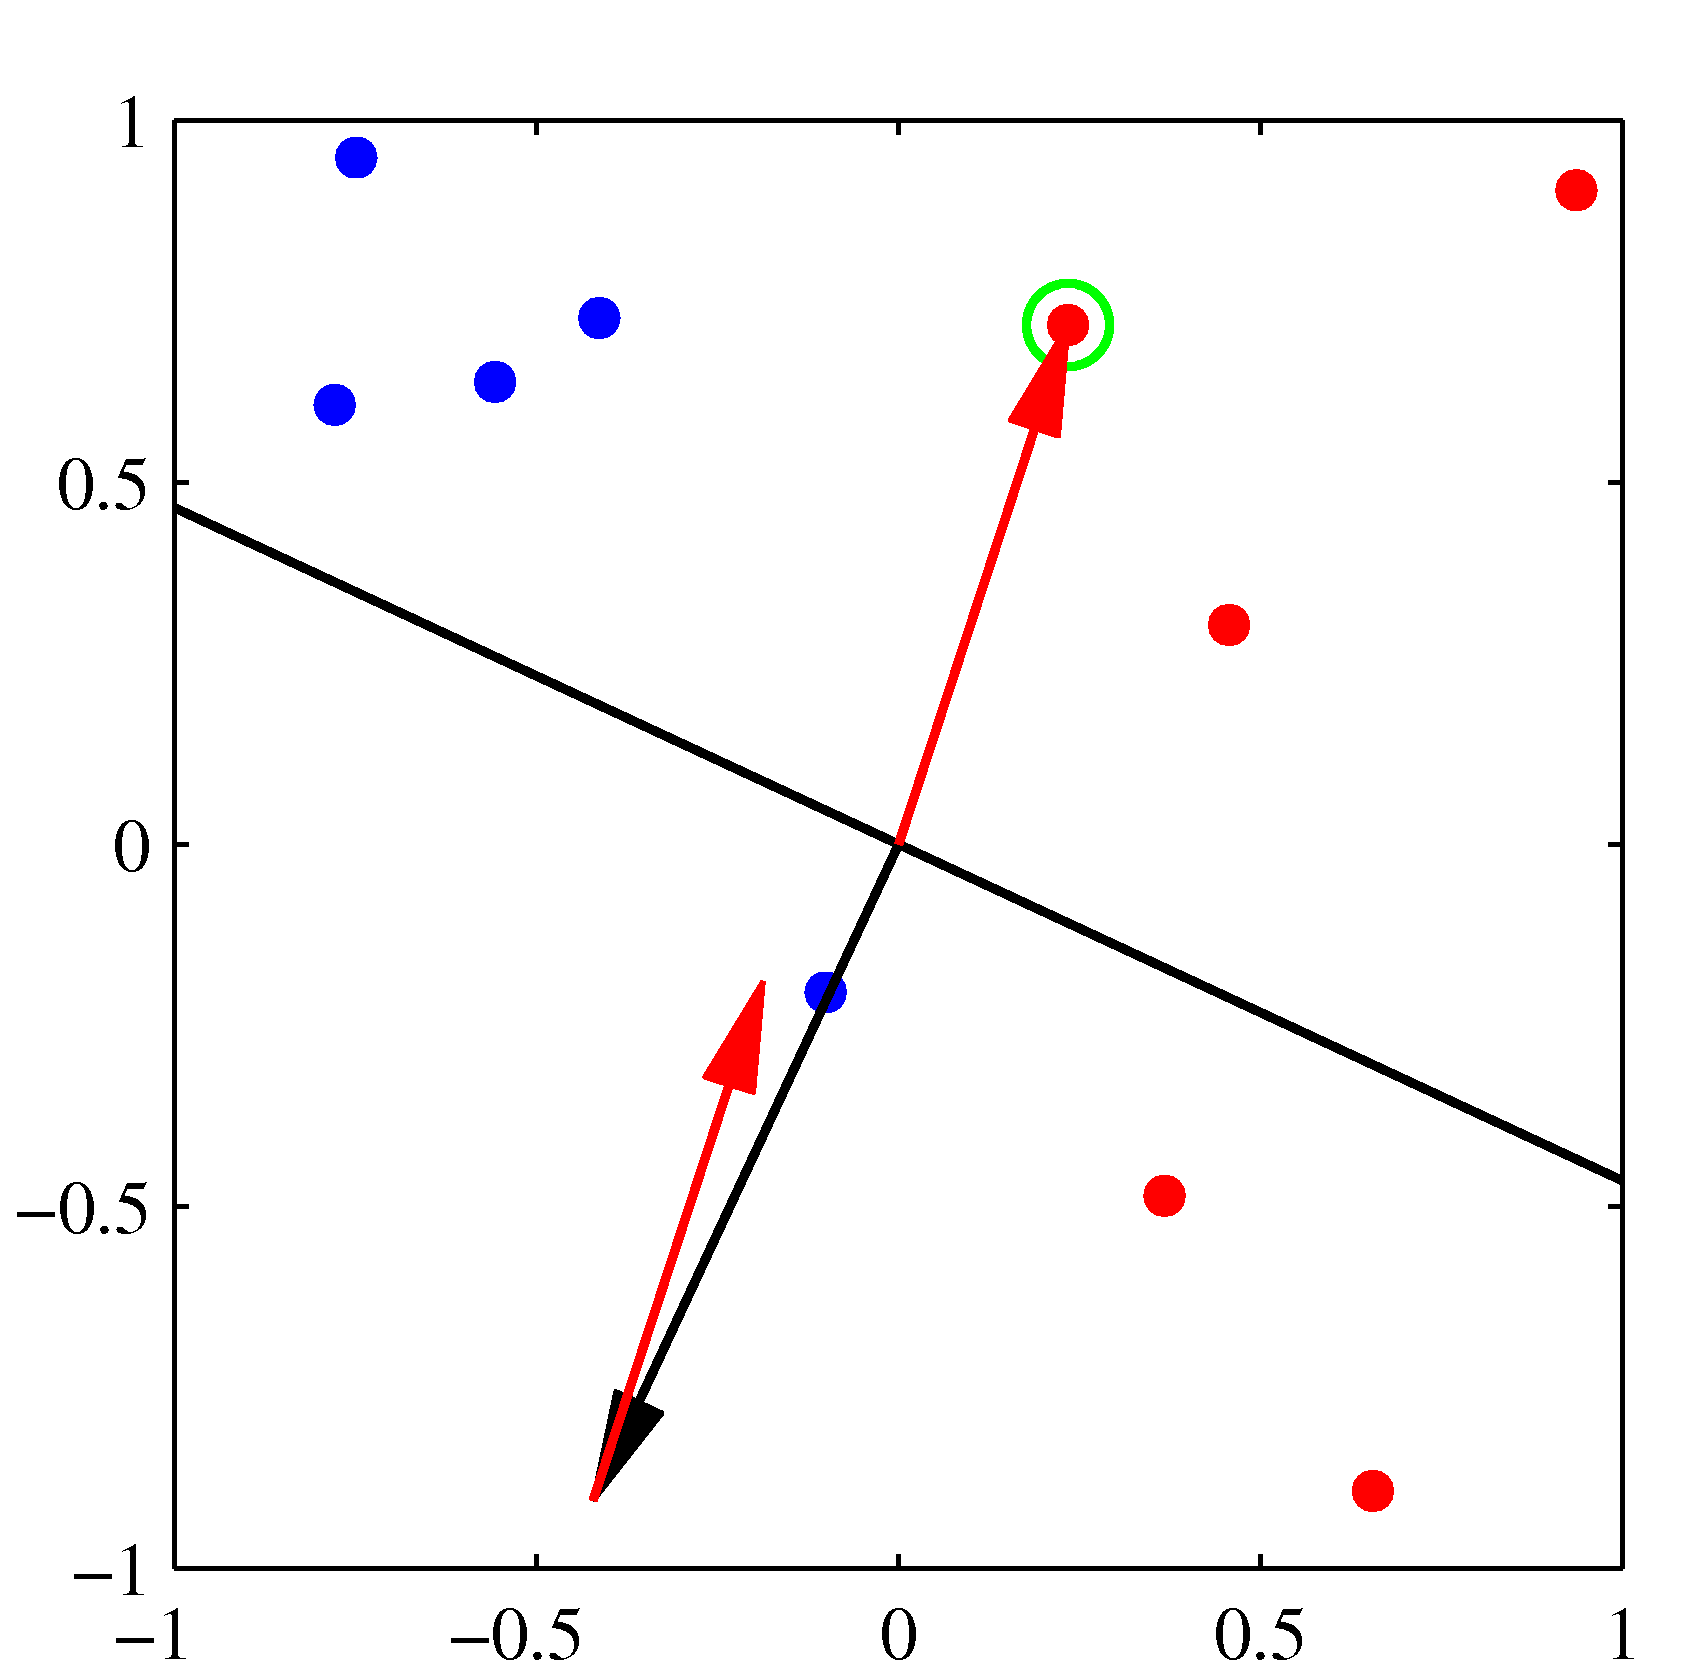
\includegraphics[scale=0.8]{Images/4-7a.png}
		\label{fig:4-7a}
		\end{minipage}
		\begin{minipage}[t]{0.5\linewidth}
		\centering
		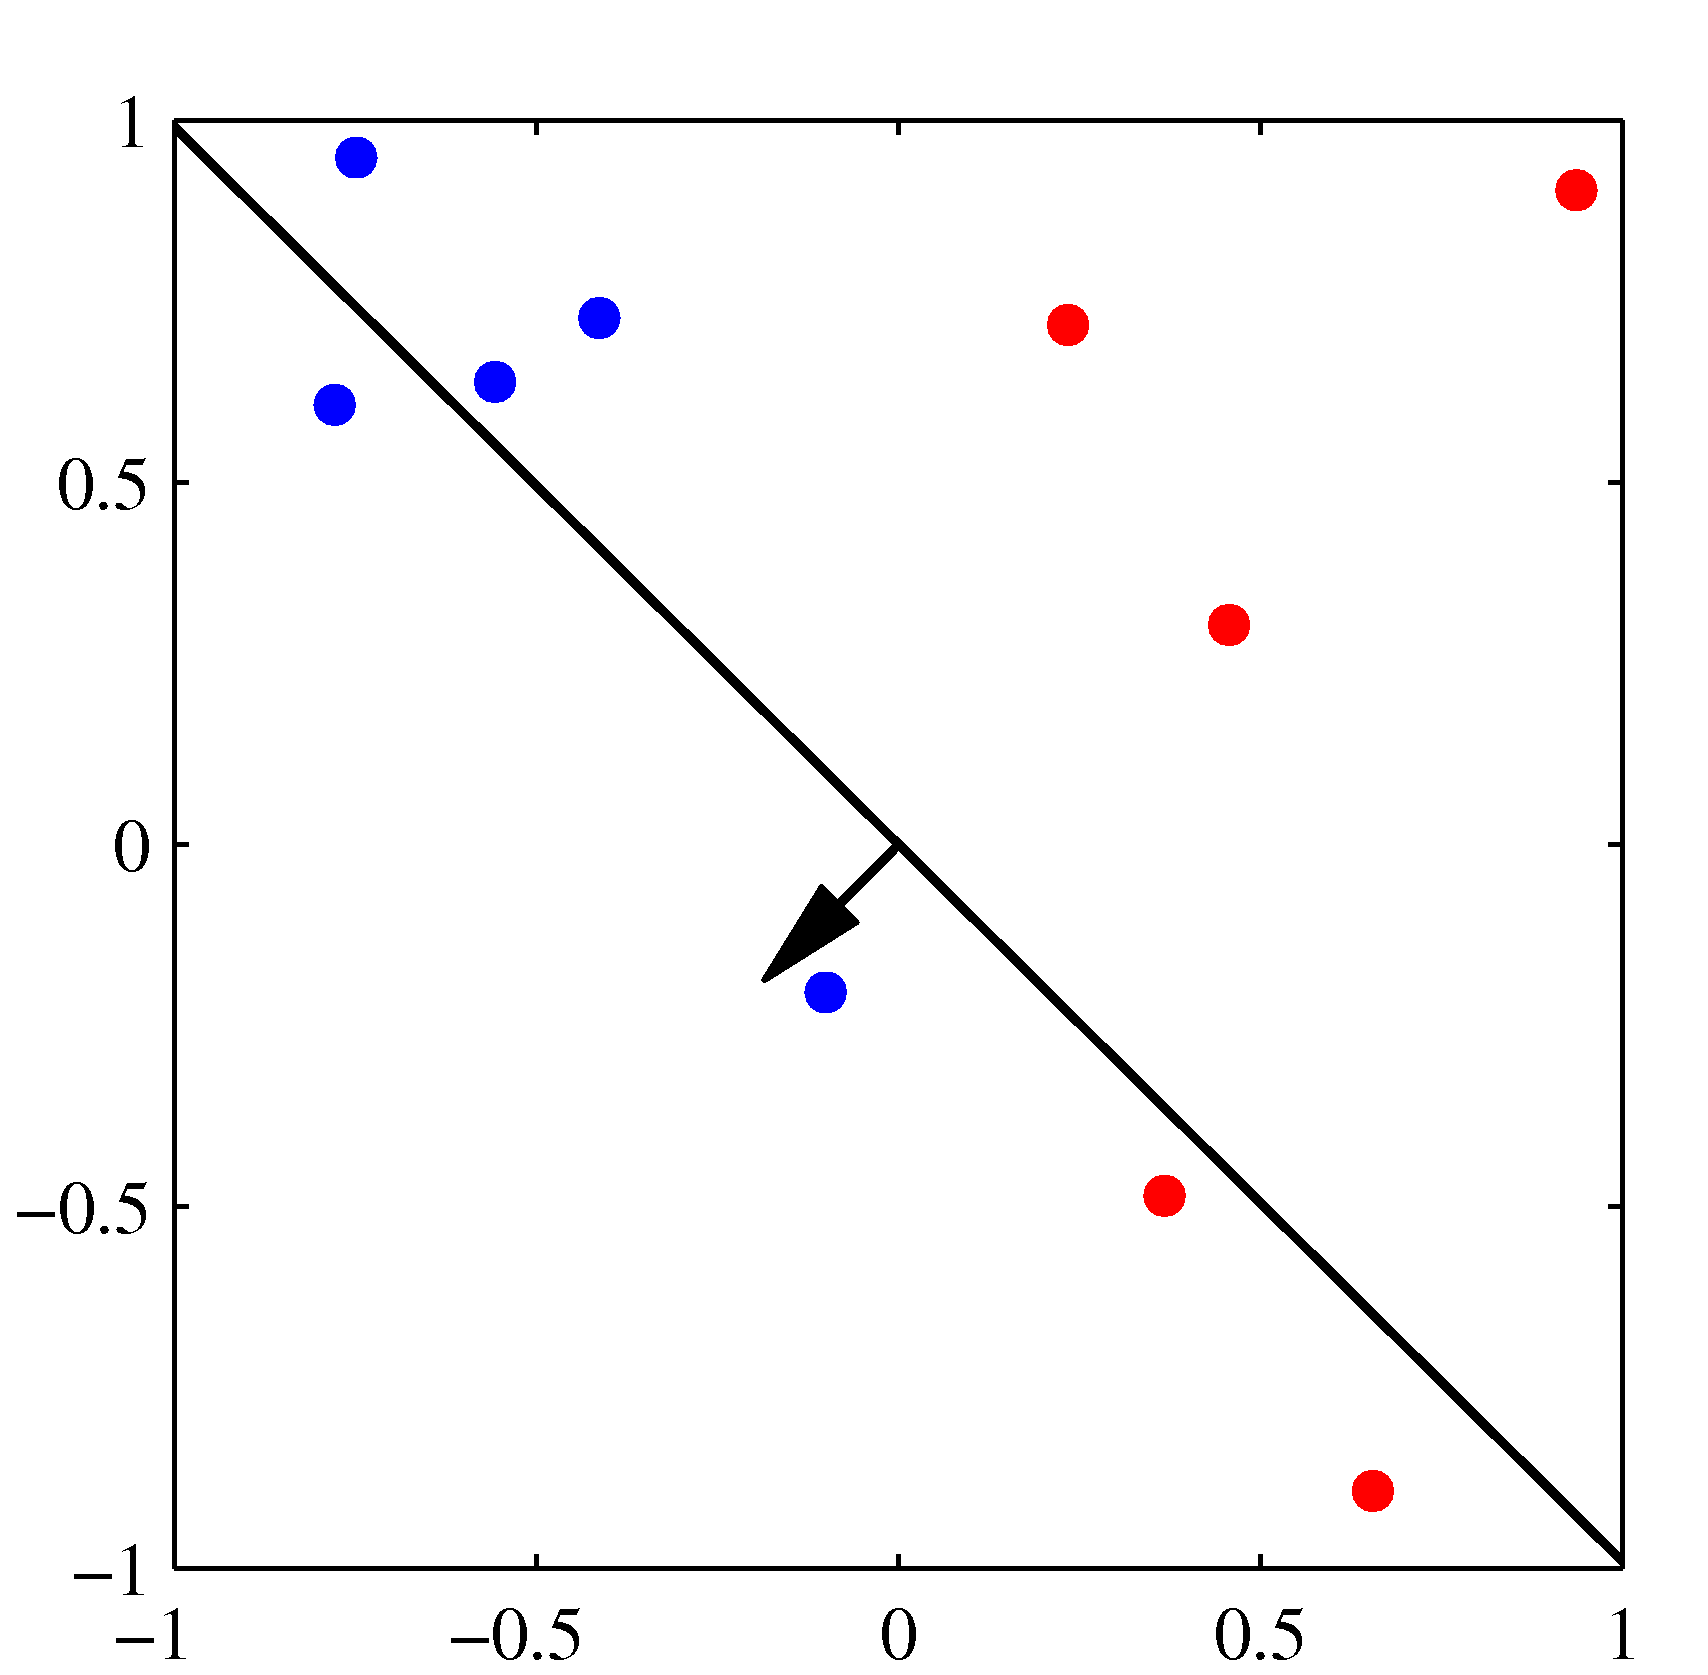
\includegraphics[scale=0.8]{Images/4-7b.png}
		\label{fig:4-7b}
		\end{minipage} \\
		\begin{minipage}[t]{0.5\linewidth}
		\centering
		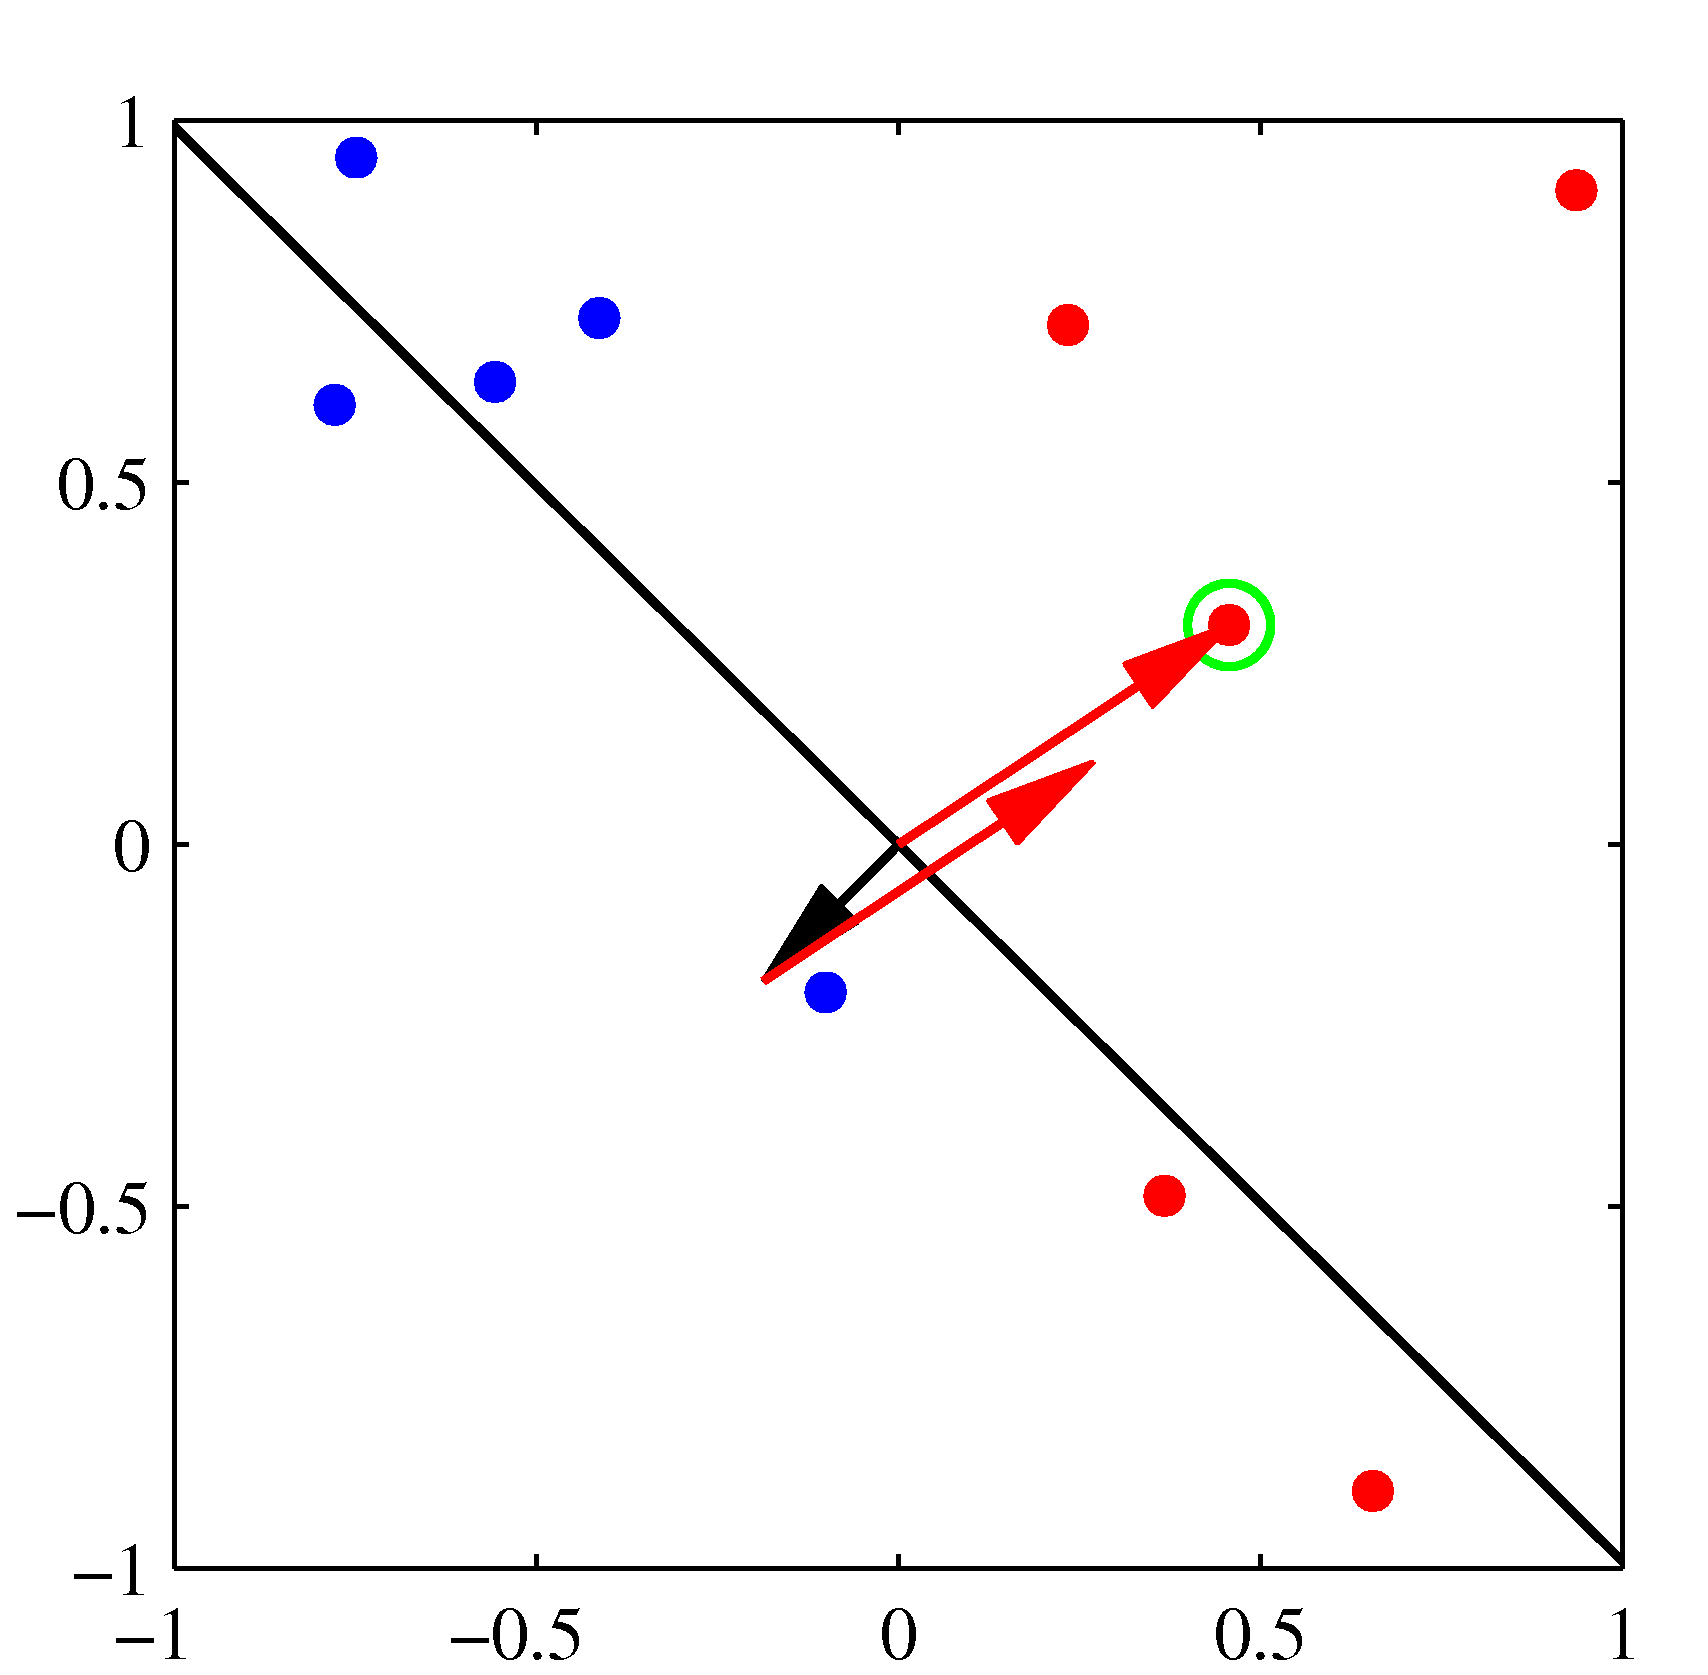
\includegraphics[scale=0.8]{Images/4-7c.png}
		\label{fig:4-7c}
		\end{minipage}
		\begin{minipage}[t]{0.5\linewidth}
		\centering
		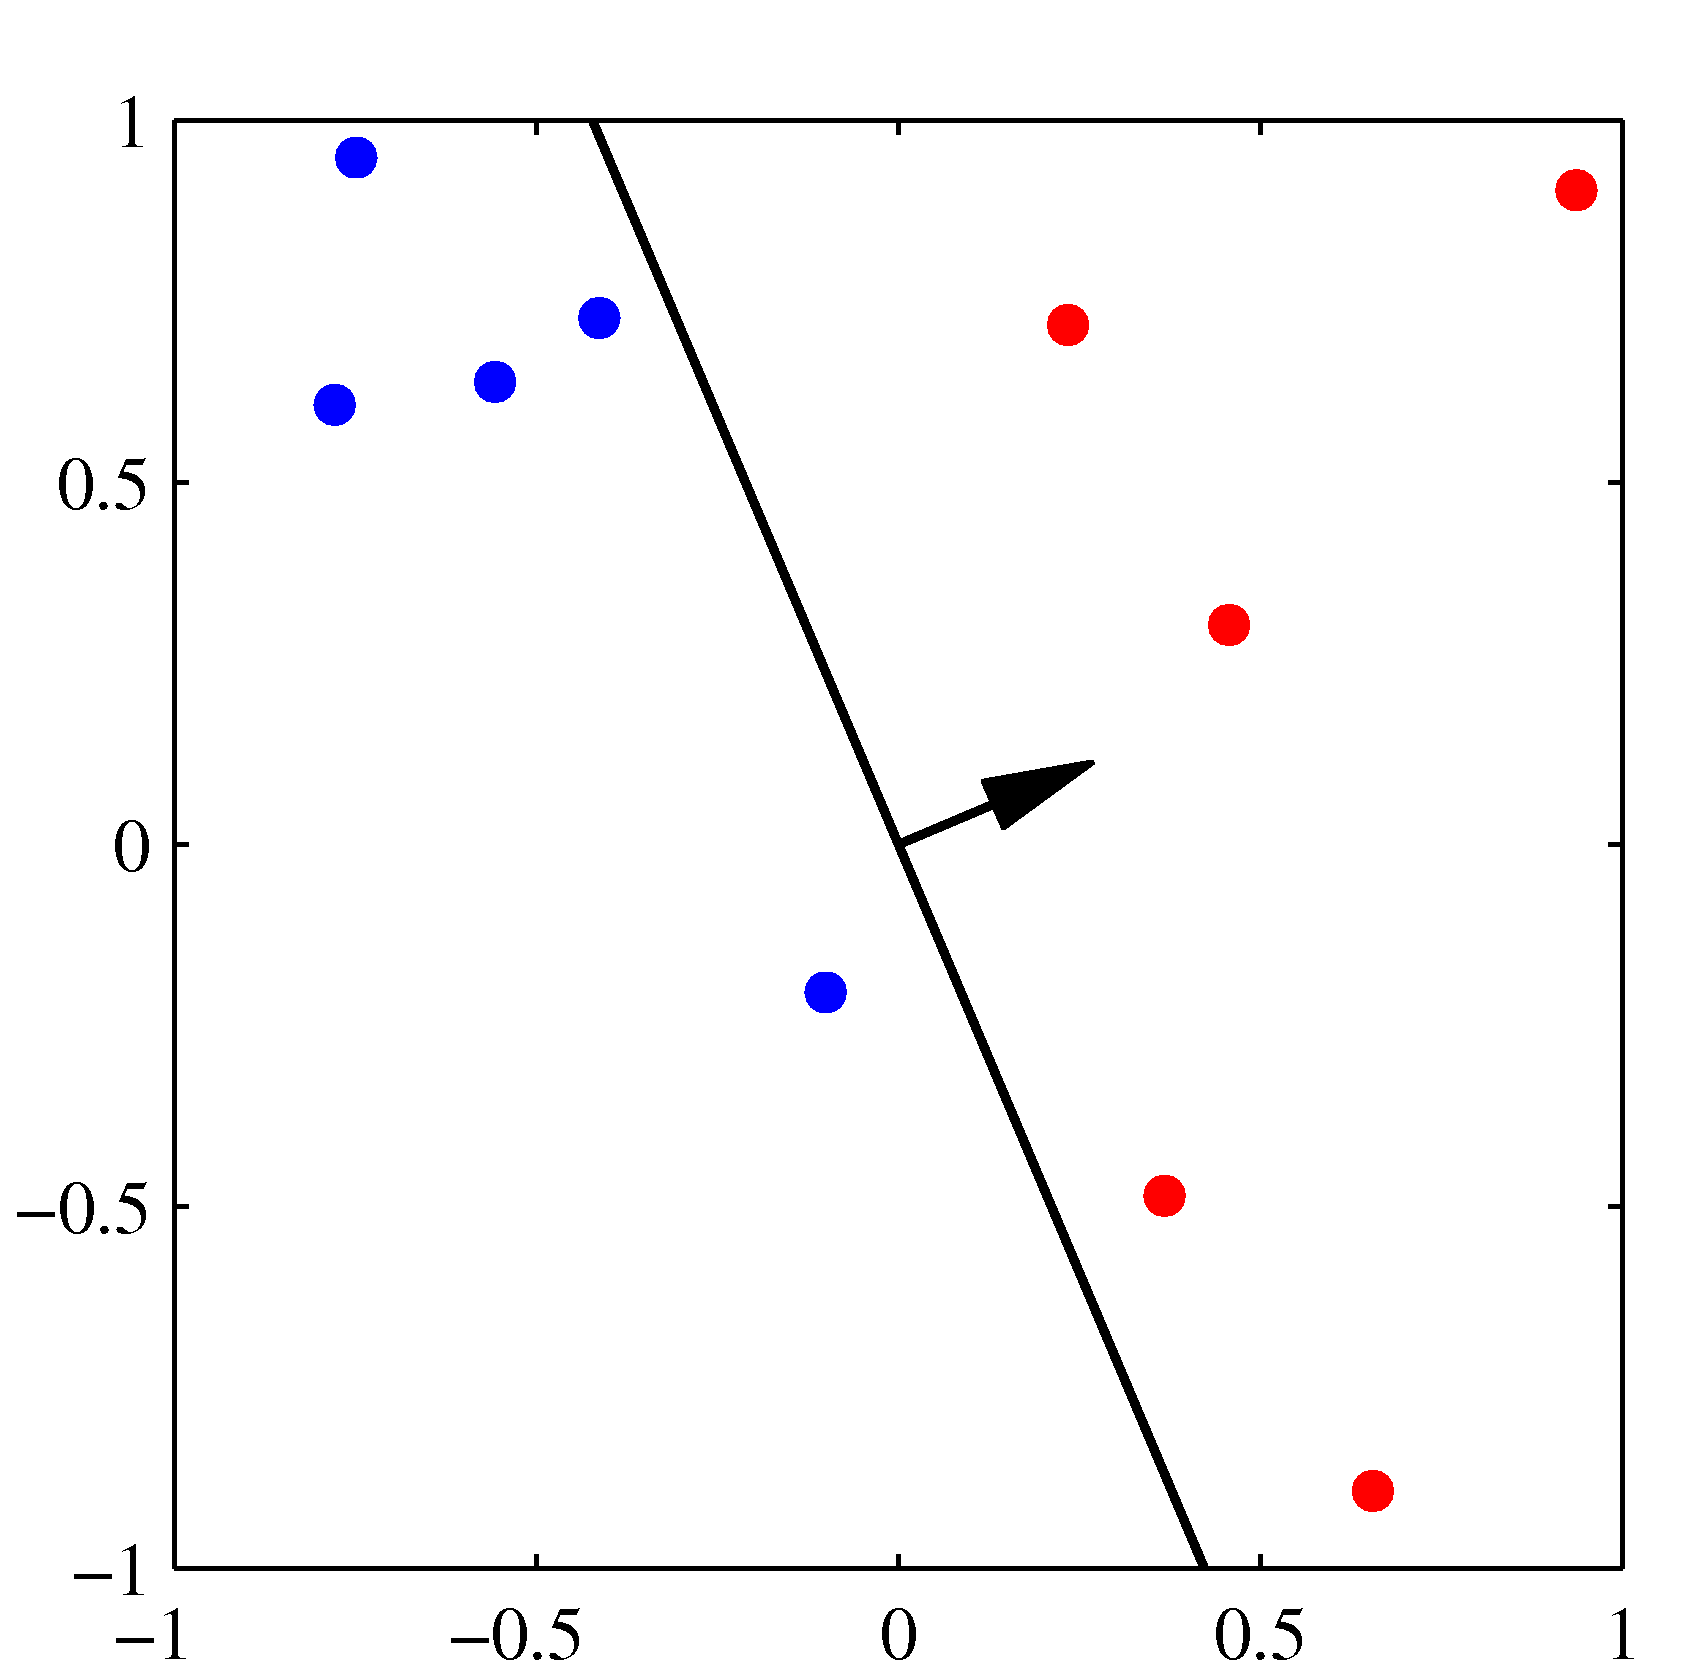
\includegraphics[scale=0.8]{Images/4-7d.png}
		\label{fig:4-7d}
		\end{minipage}
		\captionsetup{font={small}}
		\caption{感知器学习算法的收敛过程,这里展示了在二维特征空间$(\phi_1,\phi_2)$中两个类别(红色和蓝色)的数据点。左上图中的黑色箭头为初始参数向量$\bw$,黑线为相应的决策边界,箭头指向的区域为红色类别的决策区域。绿色圈出的数据点为错误分类点,因此其特征向量被添加到当前的权重向量中,从而在右上图中得到了新的决策边界。左下图展示的是下一个要考虑的错误分类点,由绿色圆圈表示,并将其特征向量再次添加到权重向量中,从而得到右下图中的决策边界,这次所有数据点的分类都正确了。}
		\centering
		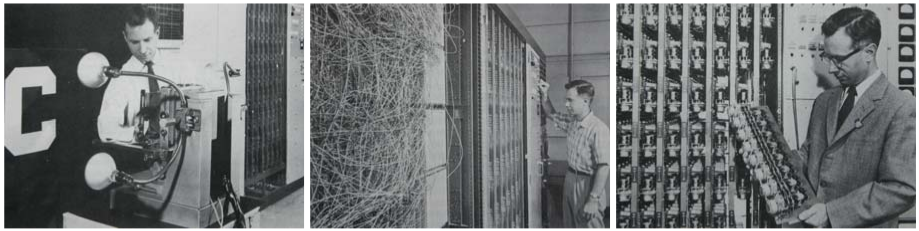
\includegraphics[scale=0.005]{Images/4-8.png}
		\captionsetup{font={small}}
		\caption{这段是介绍历史,还特别长,就不翻译了哈。。。【逃跑】}
		\label{fig:4-8}
	\end{figure}
	}
	\section{概率生成模型}
	\insertline
	\textnormal{
	\indent 现在我们换个思路,从分类模型的概率视角入手,并展示如何从数据分布的简单假设得到线性决策边界。在第1.5.4节中,我们已经讨论了分类问题中判别模型和生成模型的区别。现在我们会采用生成模型,对类别条件概率密度$p(\bx|\mathcal{C}_k)$和$\mathcal{C}_k$进行建模,然后利用它们根据贝叶斯定理计算后验概率$p(\mathcal{C}_k|\bx)$。\\
	\indent 首先研究二分类问题。类别$\mathcal{C}_1$的后验概率可以表示为
	\begin{equation}
		p(\mathcal{C}_1|\bx)= \frac{p(\bx|\calC_1)p(\calC_1)}{p(\bx|\calC_1)p(\calC_1)+p(\bx|\calC_2)p(\calC_2)} = \frac{1}{1+\exp(-a)} = \sigma(a)
	\end{equation}
	其中,
	\begin{equation}
		a = \ln \frac{p(\bx|\calC_1)p(\calC_1)}{p(\bx|\calC_2)p(\calC_2)}
	\end{equation}
	另外,$\sigma(a)$表示的是logistic sigmoid函数,定义为
	\begin{equation}
		\sigma(a) = \frac{1}{1+\exp(-a)}
	\end{equation}
	其图像如图4.9所示。“sigmoid”是“S型”的意思。这一类型的函数有时也被称为“挤压函数”(squashing function),因为它可以将整个实轴映射到有限的区间内。logistic sigmoid函数在早些时候已经提到过了,扮演了很多分类问题中的重要角色。
	\begin{figure}[ht]
		\centering
		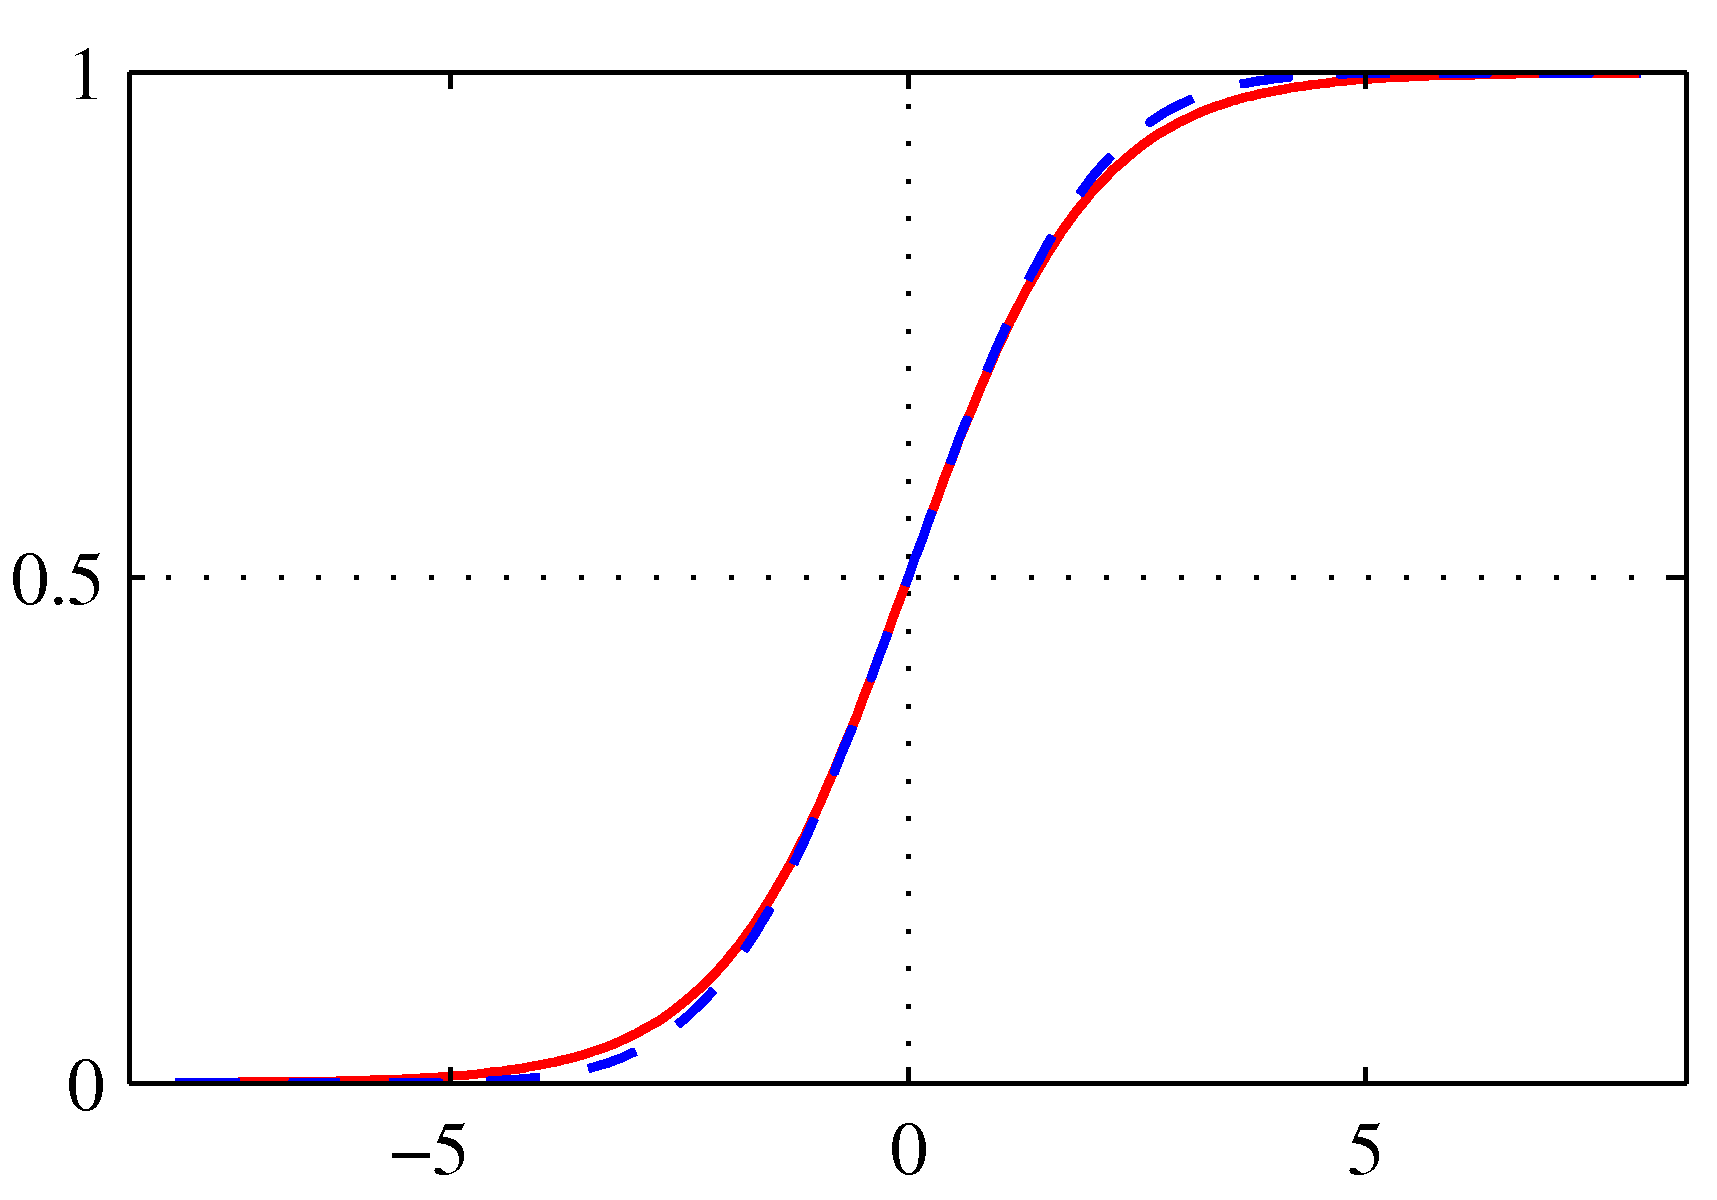
\includegraphics[scale=0.8]{Images/4-9.png}
		\captionsetup{font={small}}
		\caption{公式(4.59)所定义的logistic sigmoid函数$\sigma(a)$的函数图像(红色曲线),同时展示了经过放缩的逆概率函数(inverse probit function)$\Phi(\lambda a)$,其中$\lambda^2 = \pi/8$(蓝色虚线),$\Phi(a)$的定义详见公式(4.114)。放缩因子$\pi/8$是为了让两个函数在$a=0$的时候具有相同的函数值。}
		\label{fig:4-9}
	\end{figure}
	\\
	\textcolor{red}{【译者注:关于logistic sigmoid函数的翻译一直是个老大难问题。《统计学习方法》(李航)采用了“逻辑斯谛函数”的直接音译,《机器学习》(周志华)将logistic function称为“对数几率函数”。译者私以为原本的英文说法更能让人体会到该函数的特点,故在这里保留了logistic sigmoid函数这样的写法。】}\\
	\indent logistic sigmoid函数满足如下的对称性质:
	\begin{equation}
		\sigma(-a) = 1 - \sigma(a)
	\end{equation}
	这个很容易就可以证明了。logistic sigmoid函数的反函数为
	\begin{equation}
		a = \ln \left(\frac{\sigma}{1-\sigma}\right)
	\end{equation}
	这个函数称为logit函数。它表示的是概率的比值$\ln [p(\calC_1|\bx)/p(\calC_2|\bx)]$,同时也称为log odds。\\
	\indent 在(4.57)中,我们将后验概率写成了比较简单的等价形式,所以logistic sigmoid函数的定义可能显得比较空洞。不过,如果$a(x)$的函数形式比较简单,那么这样做是很有意义的。接下来我们就会研究$a(\bx)$为线性函数的情况,在这种情况下,后验概率是由广义线性模型得到的。\\
	\indent 对于$K>2$的分类问题,
	\begin{equation}
		p(\calC_k|\bx) = \frac{p(\bx|\calC_k)p(\calC_k)}{\sum_j p(\bx|\calC_j)p(\calC_j)} = \frac{\exp(a_k)}{\sum_j \exp(a_j)}
	\end{equation}
	这个公式为归一化指数(normalized exponential),可以看成是logistic sigmoid在多类别情况下的推广形式。其中,$a_k$的值为
	\begin{equation}
		a_k = \ln(p(\bx|\calC_k)p(\calC_k))
	\end{equation}
	归一化指数也被称为softmax函数。对于一切$j \neq k$,如果$a_k \gg a_j$,那么$p(\calC_k|\bx) \approx 1$,$p(\calC_j|\bx) \approx 0$。\\
	\indent 现在我们研究一个问题,如果将类别条件概率密度选取了特定的形式,会造成怎样的后果。首先研究$\bx$为连续输入变量的情况,然后研究离散输入的情况。
	}
	\subsection{输入量为连续变量的情况}
	\textnormal{假设类别条件概率密度为高斯分布。在开始阶段,我们首先假设所有的类别都具有相同的协方差矩阵。于是,类别$\calC_k$的概率密度为
	\begin{equation}
		p(\bx|\calC_k) = \frac{1}{(2\pi)^{D/2}}\frac{1}{|\bfSigma|^{1/2}}\exp\left\{-\frac{1}{2}(\bx - \bfMu_k)^{\rmT} \bfSigma^{-1} (\bx - \bfMu_k)\right\}
	\end{equation}
	对于二分类问题,根据(4.57)和(4.58),
	\begin{equation}
		p(\calC_1|\bx) = \sigma(\bw^{\rmT}\bx +w_0)
	\end{equation}
	其中,
	\begin{align}
		\bw &= \bfSigma^{-1} (\bfMu_1 - \bfMu_2)\\
		w_0 &= -\frac{1}{2}\bfMu_1^{\rmT}\bfSigma^{-1}\bfMu_1 + \frac{1}{2}\bfMu_2^{\rmT}\bfSigma^{-1}\bfMu_2 + \ln \frac{p(\calC_1)}{p(\calC_2)}
	\end{align}
	可以看出由高斯概率密度函数的指数项而来的关于$\bx$的二次项消失了,因为我们做出了关于协方差矩阵的假设,于是logistic sigmoid函数的自变量就变成了关于$\bx$的线性函数。如图4.10所示的是当输入空间$\bx$为二维空间时的情况。由此得到的决策边界所对应的是后验概率$p(\calC_k|\bx)$为常数的曲面,由于是关于$\bx$的线性函数,所以决策边界也是输入空间中的线性函数。先验概率$p(\calC_k)$仅仅会对偏差参数$w_0$产生影响,所以先验的变化会使决策边界发生平移,也就是平移后验概率的常数轮廓线。
	\begin{figure}[H]
		\begin{minipage}[t]{0.5\linewidth}
		\centering
		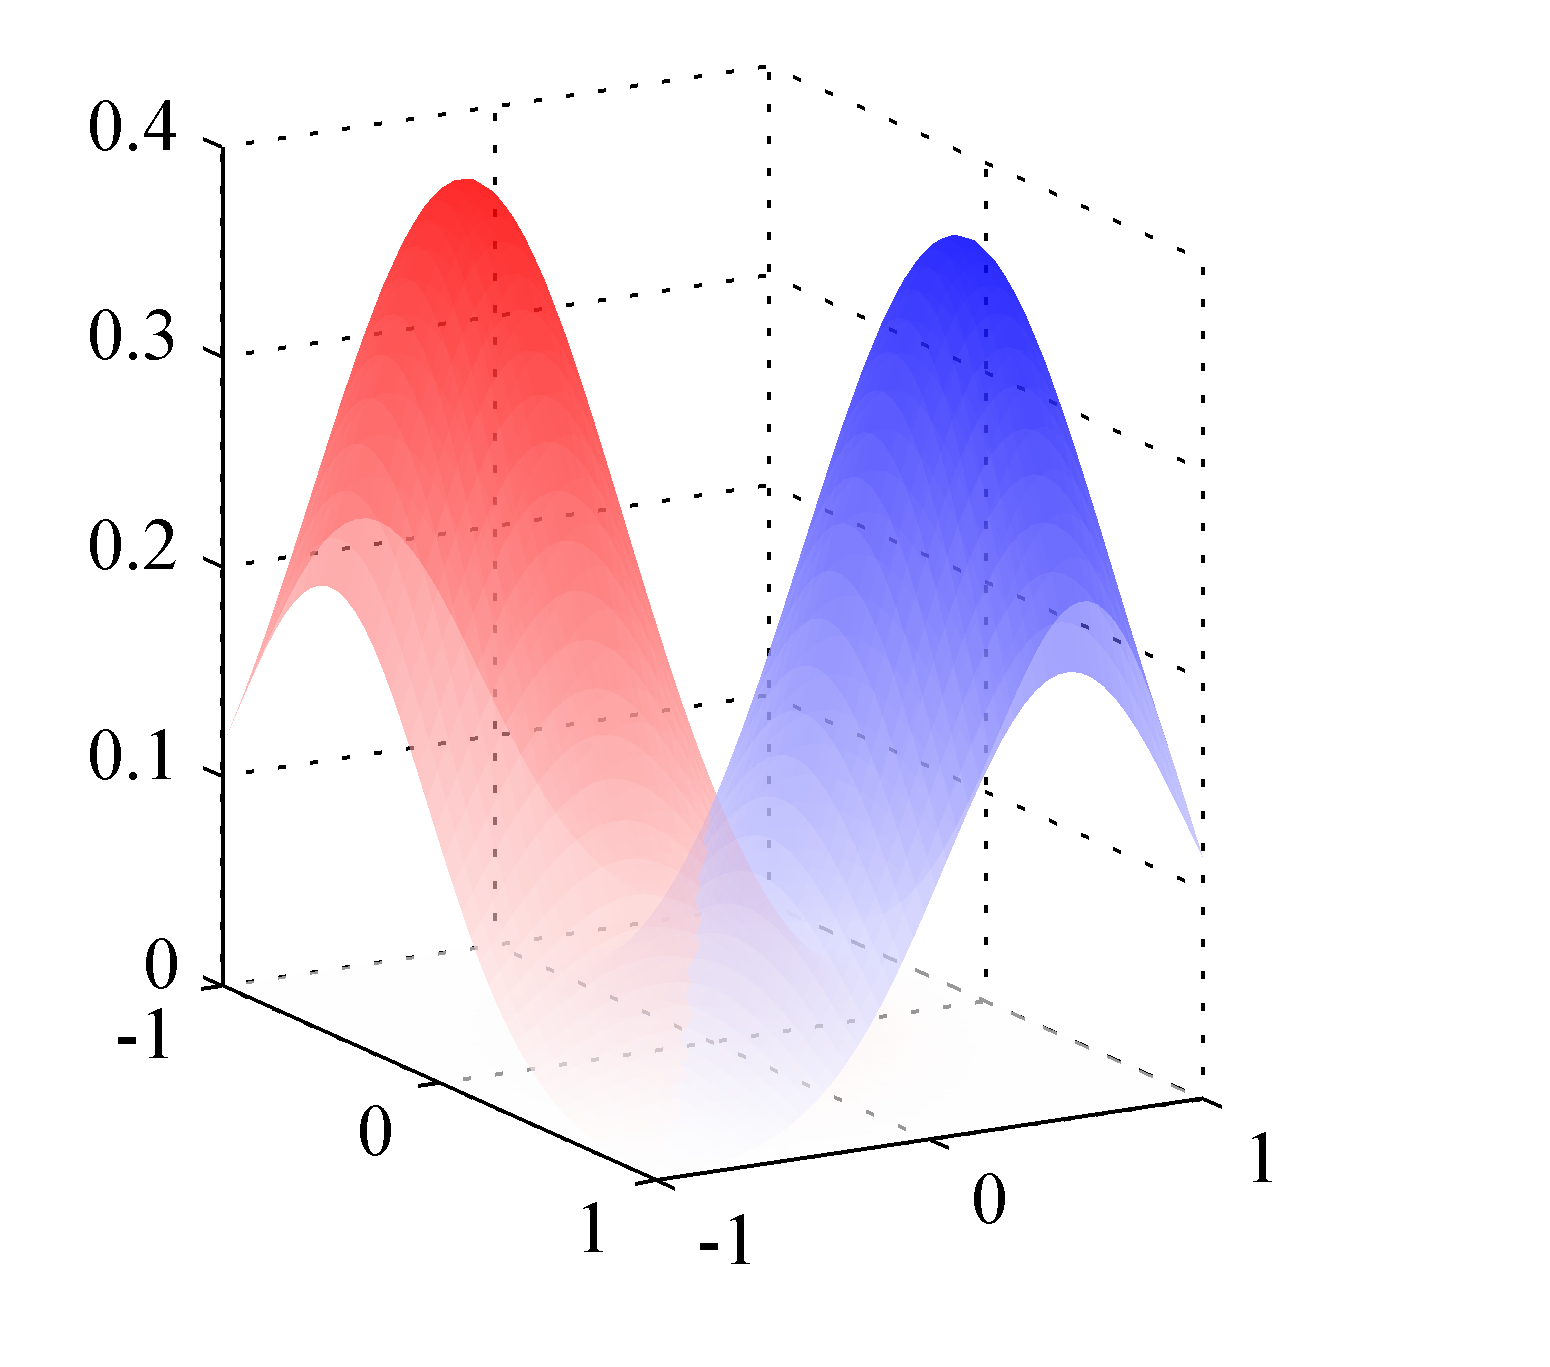
\includegraphics[scale=0.8]{Images/4-10a.png}
		\label{fig:4-10a}
		\end{minipage}
		\begin{minipage}[t]{0.5\linewidth}
		\centering
		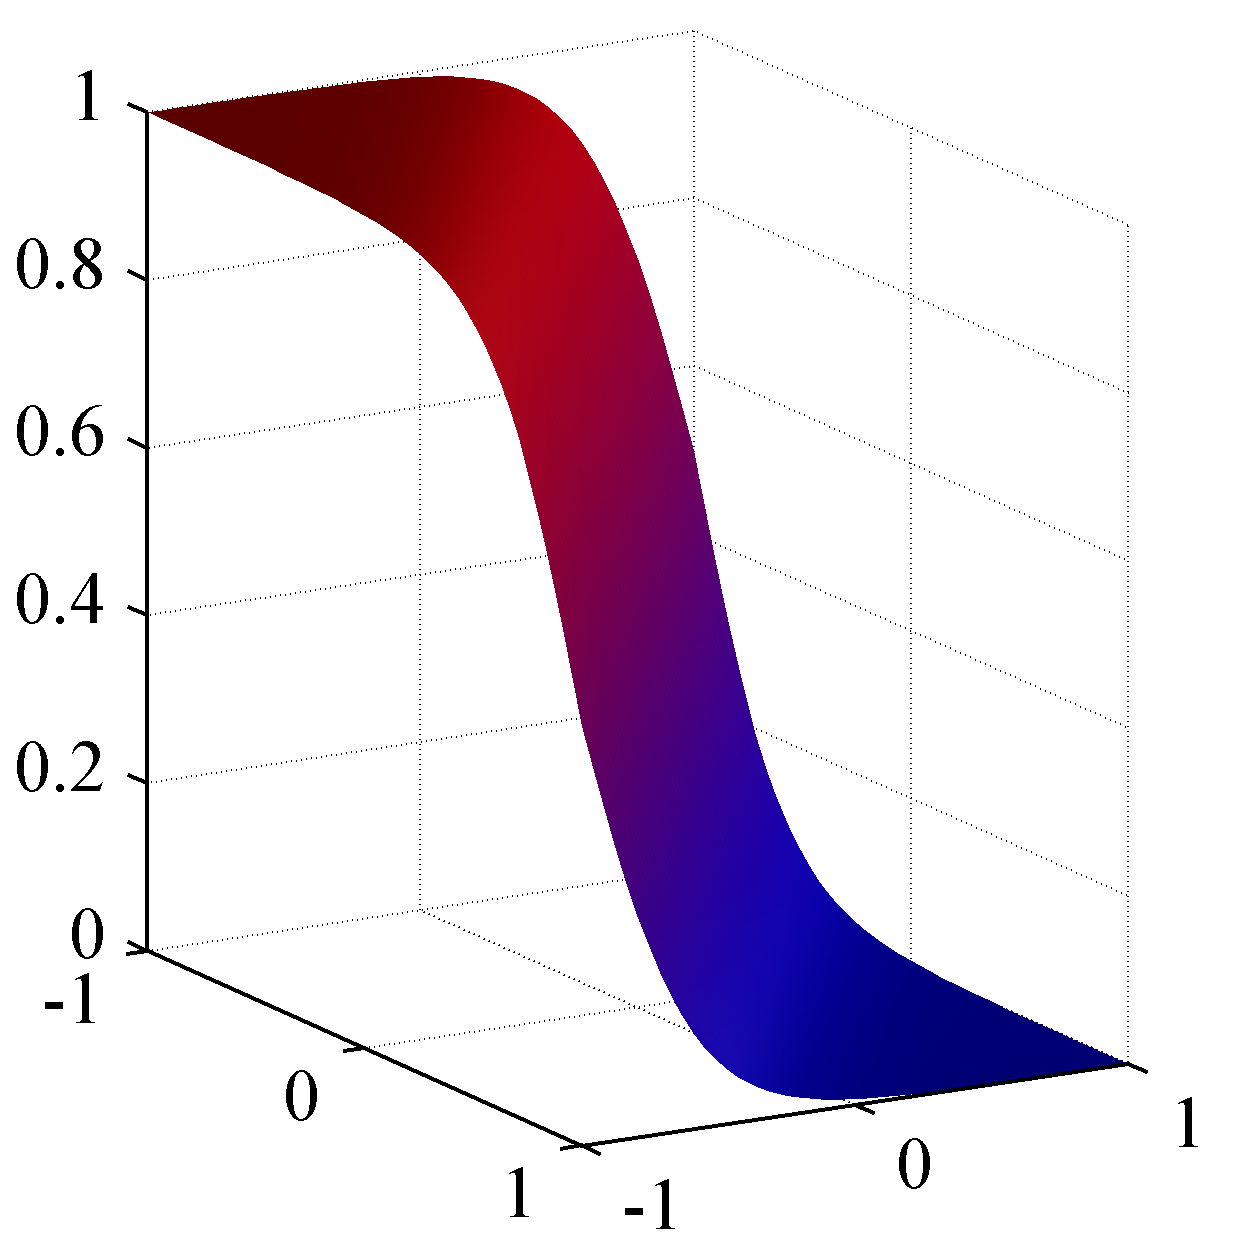
\includegraphics[scale=0.8]{Images/4-10b.png}
		\label{fig:4-10b}
		\end{minipage}
		\captionsetup{font={small}}
		\caption{左图展示的是两个类别的类别条件概率密度,分别表示为红色和蓝色。右图为对应的后验概率$p(\calC_1|\bx)$,它是一个以$\bx$的线性函数为自变量的logistic sigmoid函数。右图的曲面采用了渐变色,红色表示$p(\calC_1|\bx)$,蓝色表示$p(\calC_2|\bx)=1-p(\calC_2|\bx)$,所以整个曲面呈现了从红到蓝的变化过程。}
	\end{figure}
	\indent 对于$K$分类问题,根据(4.62)和(4.63),
	\begin{equation}
		a_k(\bx) = \bw_k^{\rmT}\bx + w_{k0}
	\end{equation}
	其中,
	\begin{align}
		\bw_k &= \bfSigma^{-1}\bfMu_k \\
		w_{k0} &= -\frac{1}{2}\bfMu_k^{\rmT}\bfSigma^{-1}\bfMu_k + \ln p(\calC_k)
	\end{align}
	\begin{figure}[ht]
		\begin{minipage}[t]{0.5\linewidth}
		\centering
		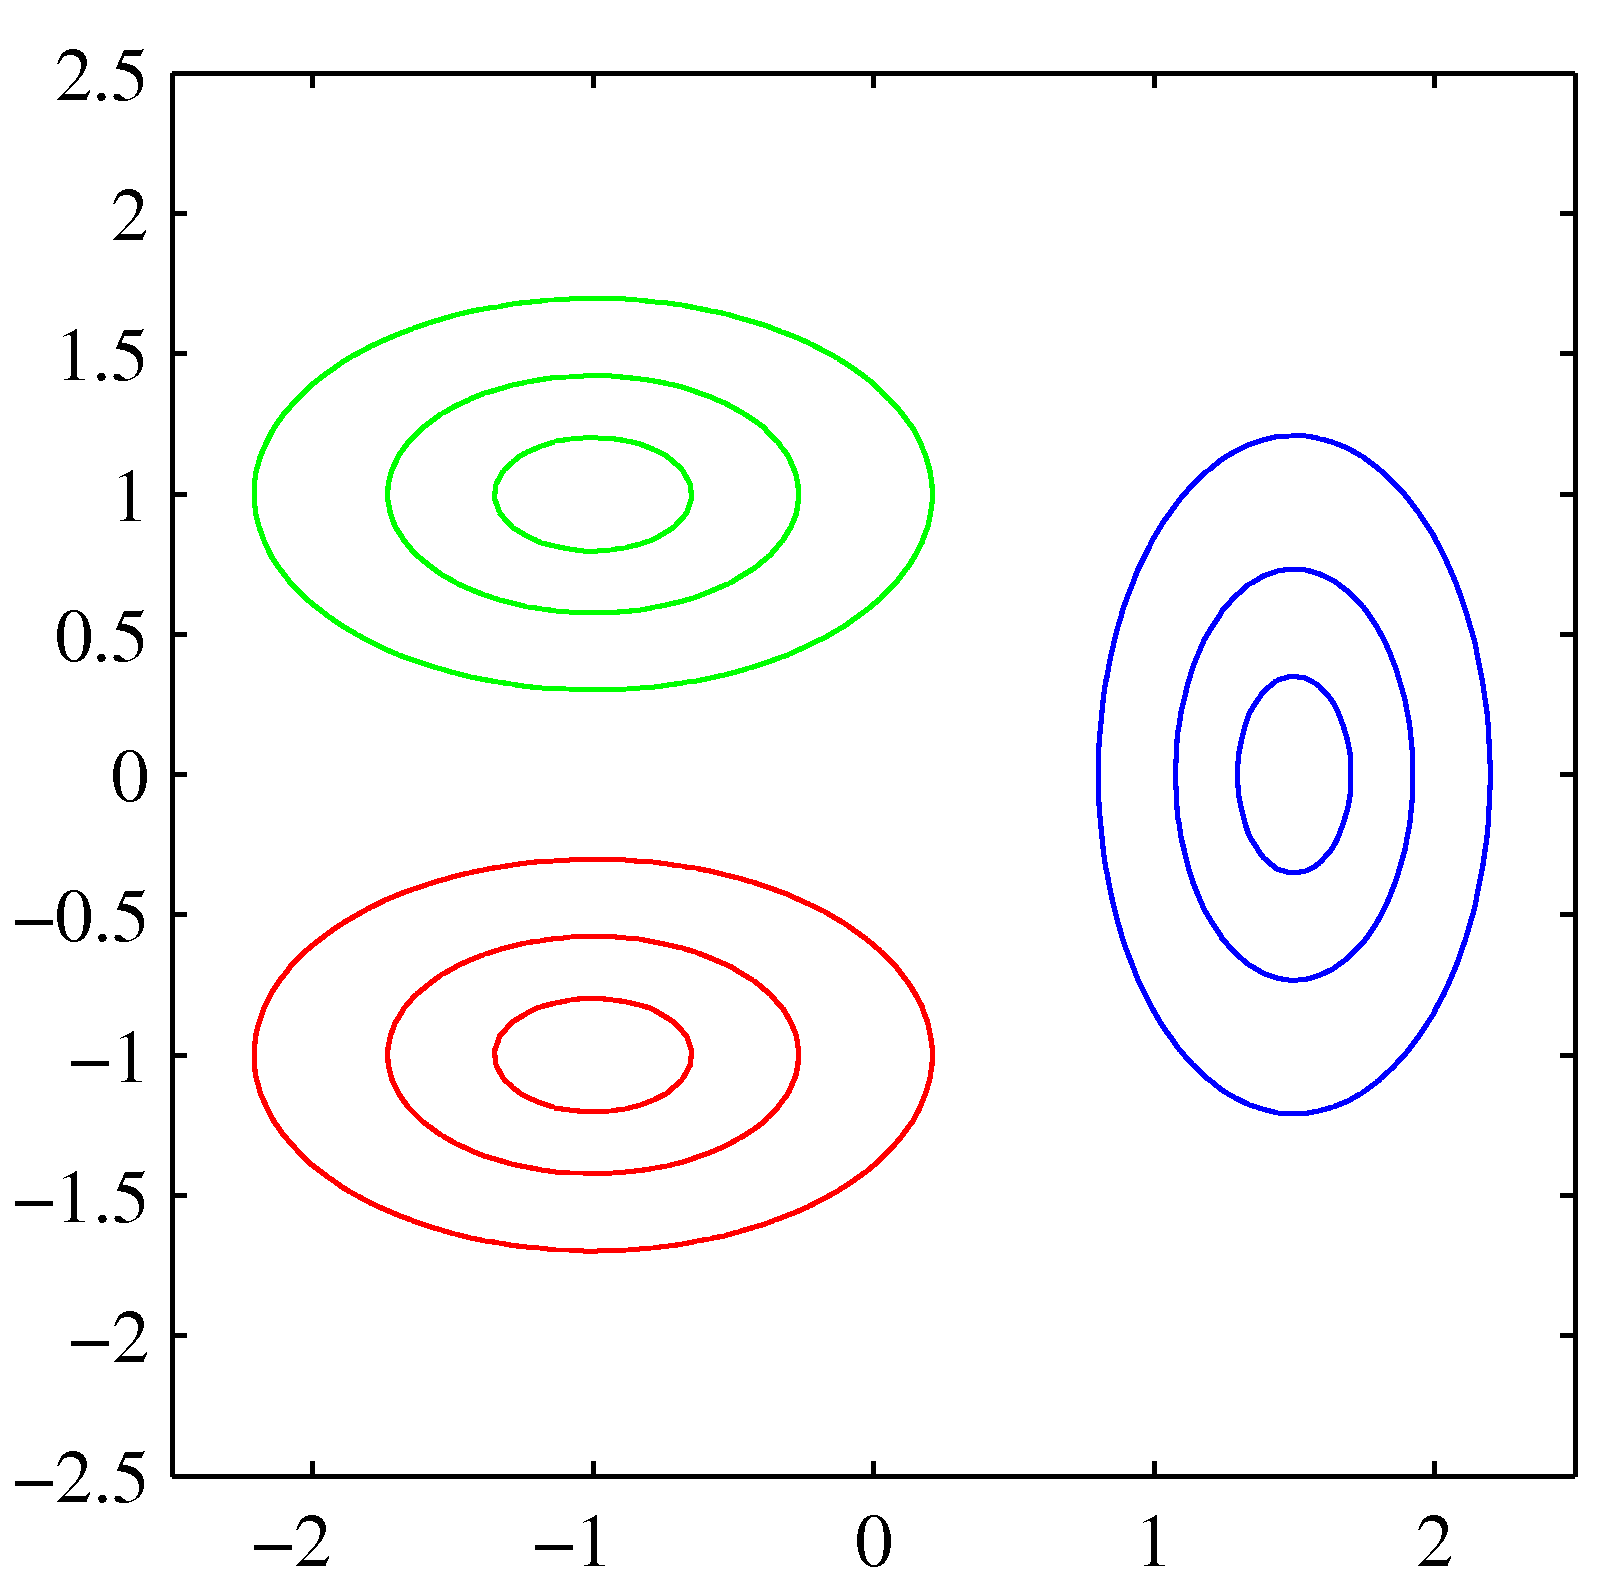
\includegraphics[scale=0.8]{Images/4-11a.png}
		\label{fig:4-11a}
		\end{minipage}
		\begin{minipage}[t]{0.5\linewidth}
		\centering
		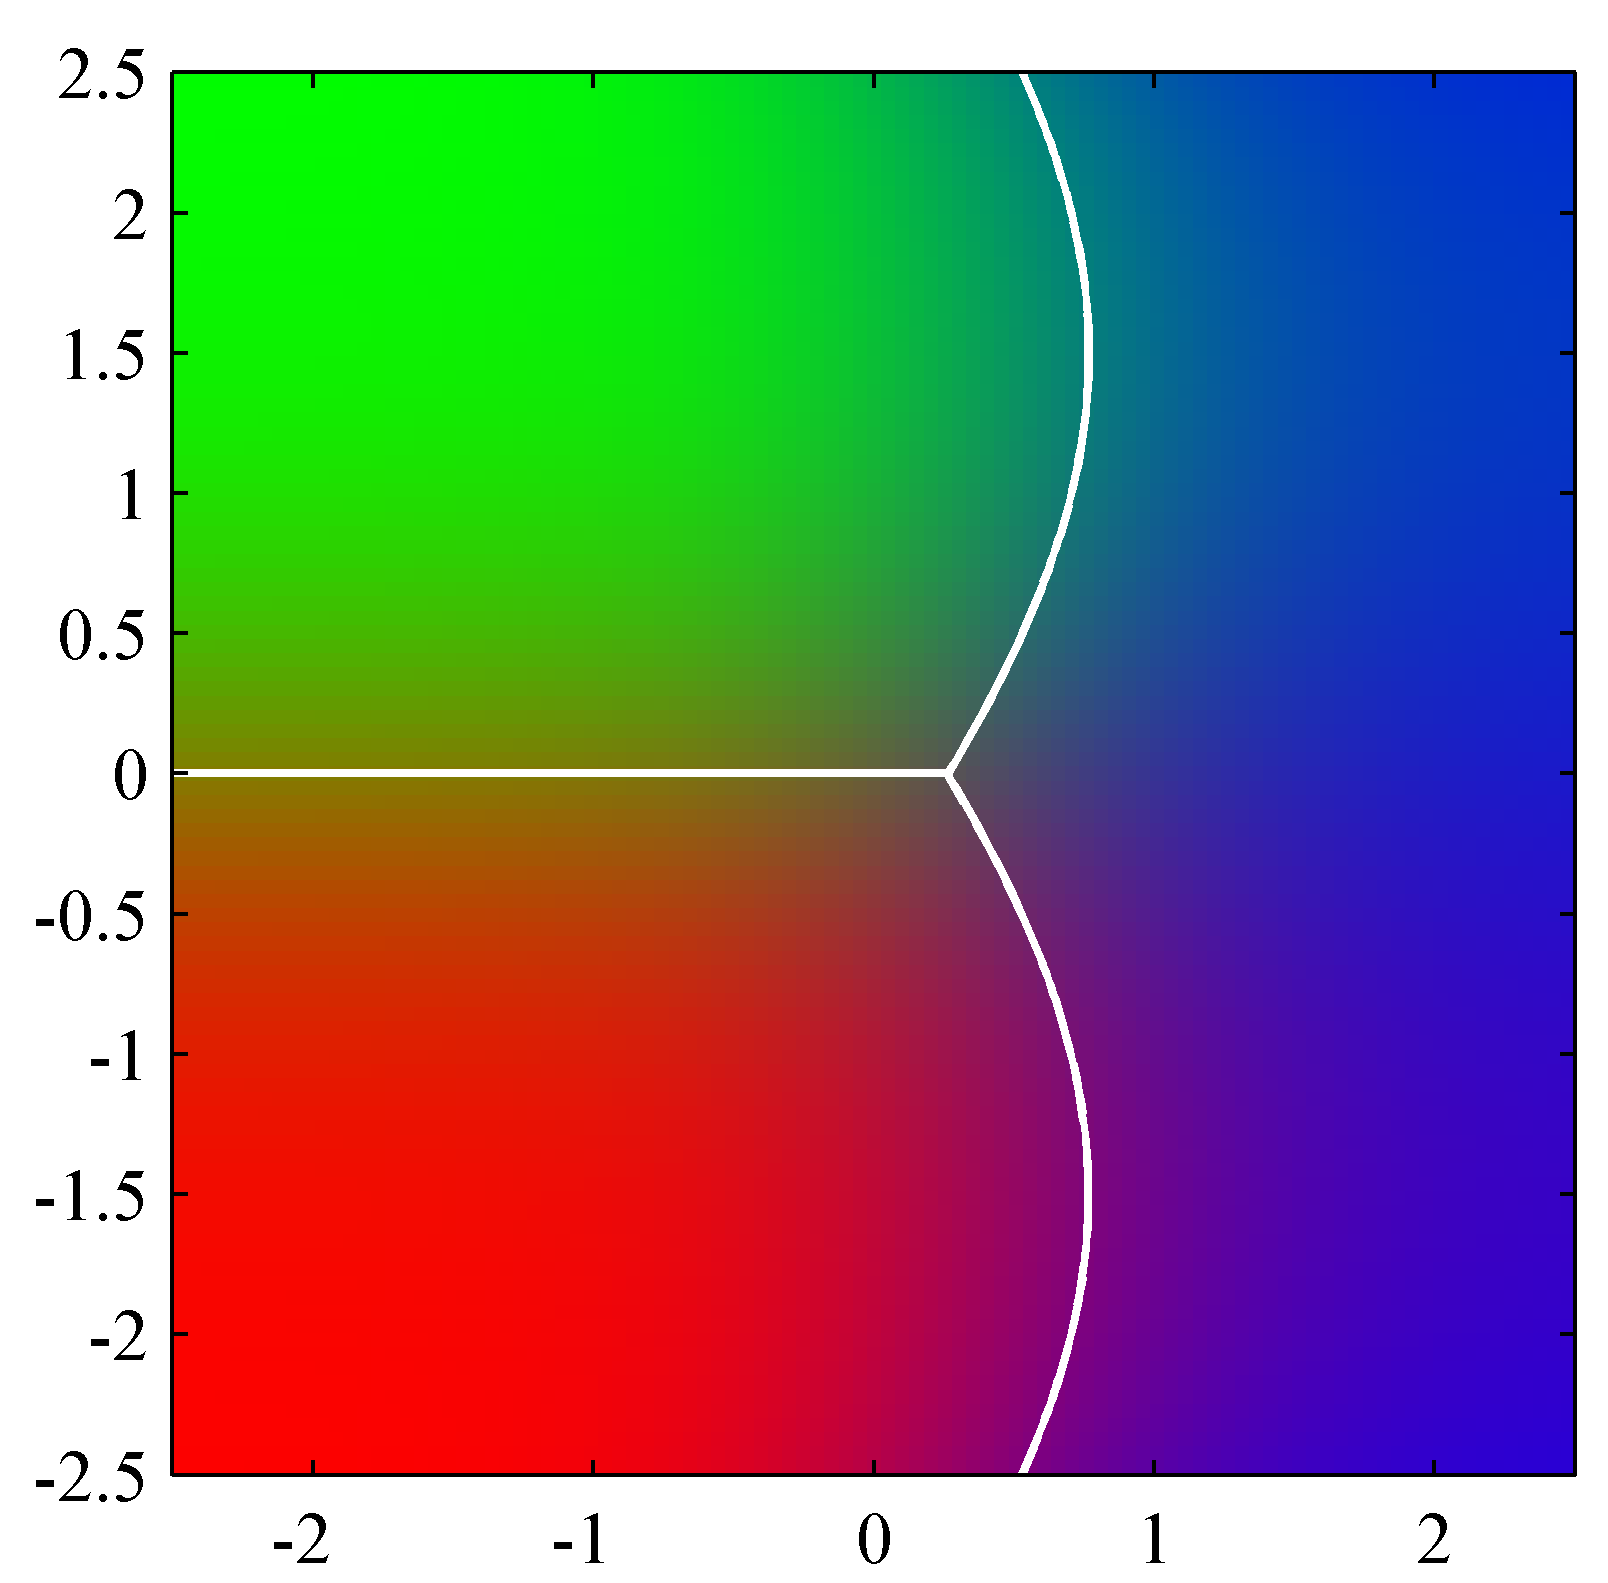
\includegraphics[scale=0.8]{Images/4-11b.png}
		\label{fig:4-11b}
		\end{minipage}
		\captionsetup{font={small}}
		\caption{左图显示了三个类别的类别条件概率密度,每个类别各自对应一个高斯分布,分别表示为红色,绿色和蓝色,其中红色和绿色的类别具有相同的协方差矩阵。右图展示了相应的后验概率,其中RGB颜色矢量分别相应三个类别的后验概率。同时也展示了决策边界。需要注意的是,在具有相同协方差矩阵的红色和绿色类别之间,决策边界是线性的,而其他的边界则是二次的。}
	\end{figure}
	和之前的一样,$a_k(\bx)$又成了$\bx$的线性函数。于是,当两个最大的后验概率相等时,可以得到使得误分类率达到最小的决策边界,它是一个关于$\bx$的线性函数,于是最终得到的是一个广义线性模型。\\
	\indent 如果我们将协方差矩阵的假设放宽,允许每个类别的条件概率密度$p(\bx|\calC_k)$都有其各自的协方差矩阵$\bfSigma_k$,那么上面函数中的二次项就无法消除了,最后得到的是一个关于$\bx$的二次函数,麻烦也随之升级,变成了二次判别分析(quadratic discriminant)。线性决策边界和二次决策边界如图4.11所示。
	}
	\subsection{最大似然方法}
	\textnormal{一旦我们为类别条件概率密度$p(\bx|\calC_k)$指定了一个带参数的函数形式,配合类别先验概率$p(\calC_k)$,就可以利用最大似然方法确定函数中的参数值。这自然需要一个训练集,里面包含有$\bx$和它们各自对应的类别标签。\\
	\indent 首先分析二分类问题,假设两个类别的条件概率密度都是高斯分布,而且具有相同的协方差矩阵,以及训练集为$\{\bx_n, t_n\}, n-1,...,N$。当$t_n = 1$时表示属于类别$\calC_1$,$t_n = 0$时表示属于类别$\calC_2$。设先验概率$p(\calC_1) = \pi$,那么$p(\calC_2)$自然为$1-\pi$。对于某个属于$\calC_1$的数据$\bx_n$,有$t_n = 1$,于是
	\begin{equation*}
		p(\bx_n, \calC_1) = p(\calC_1)p(\bx_n|\calC_1) = \pi \mathcal{N}(\bx_n|\bfMu_1, \bfSigma)
	\end{equation*}
	类似地,对于类别$\calC_2$,$t_n = 0$,于是
	\begin{equation*}
		p(\bx_n, \calC_2) = p(\calC_2)p(\bx_n|\calC_2) = (1 - \pi)\mathcal{N}(\bx_n|\bfMu_2,\bfSigma)
	\end{equation*}
	于是似然函数为
	\begin{equation}
		p(\sft, \bx|\pi, \bfMu_1, \bfMu_2, \bfSigma) = \prod_{n=1}^N \left[\pi \mathcal{N}(\bx_n|\bfMu_1, \bfSigma)\right]^{t_n} \left[(1-\pi)\mathcal{N}(\bx_n|\bfMu_2,\bfSigma)\right]^{1-t_n}
	\end{equation}
	其中$\sft = (t_1, ...,t_N)^{\rmT}$。和往常一样,将其取对数之后再进行最大化会方便很多。首先关于$\pi$进行最大化。在对数似然函数中,与$\pi$有关的内容是
	\begin{equation}
		\sum_{n=1}^N \left\{t_n \ln \pi + (1-t_n)\ln (1-\pi)\right\}
	\end{equation}
	令关于$\pi$的导数为0并整理,可以得到
	\begin{equation}
		\pi = \frac{1}{N}\sum_{n=1}^N t_n = \frac{N_1}{N} = \frac{N_1}{N_1 + N_2}
	\end{equation}
	其中$N_1$表示属于类别$\calC_1$的数据总数,$N_2$表示属于类别$calC_2$的数据总数。所以和预想的一样,$\pi$的最大似然估计就是属于类别$\calC_1$的数据所占的比例。这个结论可以很轻松地推广到多分类问题中,即某一类别的先验概率等于属于该类别的数据在所有数据中所占的比例。\\
	\indent 接下来计算关于$\bfMu_1$的最大似然。仍然是将和$\bfMu_1$有关的项挑出来,
	\begin{equation}
		\sum_{n=1}^N t_n \ln \mathcal{N}(\bx_n|\bfMu_1, \bfSigma) = -\frac{1}{2}\sum_{n=1}^N t_n(\bx_n - \bfMu_1)^{\rmT}\bfSigma^{-1}(\bx_n-\bfMu_1) + \mathrm{const}
	\end{equation}
	令关于$\bfMu_1$的导数为0并整理,可以得到
	\begin{equation}
		\bfMu_1 = \frac{1}{N_1}\sum_{n=1}^N t_n \bx_n
	\end{equation}
	这事实上是所有属于类别$\calC_1$的输入向量$\bx_n$的均值。通过类似的过程,可以得到$\bfMu_2$的最大似然解
	\begin{equation}
		\bfMu_2 = \frac{1}{N_2}\sum_{n=1}^N (1-t_n) \bx_n
	\end{equation}
	也就是所有属于类别$\calC_2$的输入向量$\bx_n$的均值。\\
	\indent 最后计算协方差矩阵的最大似然解。将对数似然函数中与$\bfSigma$有关的项挑出来,
	\begin{equation}
	\begin{split}
		&-\frac{1}{2}\sum_{n=1}^N t_n \ln |\bfSigma| - \frac{1}{2}\sum_{n=1}^N t_n(\bx_n - \bfMu_1)^{\rmT}\bfSigma^{-1}(\bx_n - \bfMu_1)\\
		&-\frac{1}{2}\sum_{n=1}^N (1 - t_n) \ln |\bfSigma| - \frac{1}{2}\sum_{n=1}^N (1-t_n)(\bx_n - \bfMu_2)^{\rmT}\bfSigma^{-1}(\bx_n - \bfMu_2)\\
		&= -\frac{N}{2}\ln |\bfSigma| - \frac{N}{2}\mathrm{Tr}\left\{\bfSigma^{-1}\mathbf{S}\right\}
	\end{split}
	\end{equation}
	其中,
	\begin{align}
		\mathbf{S} &= \frac{N_1}{N}\mathbf{S}_1 + \frac{N_2}{N}\mathbf{S}_2 \\
		\mathbf{S}_1 &= \frac{1}{N_1}\sum_{n \in \calC_1}(\bx_n - \bfMu_1)(\bx_n - \bfMu_1)^{\rmT} \\
		\mathbf{S}_2 &= \frac{1}{N_2}\sum_{n \in \calC_2}(\bx_n - \bfMu_2)(\bx_n - \bfMu_2)^{\rmT}
	\end{align}
	利用高斯分布最大似然解的结论,可以看出$\bfSigma = \mathbf{S}$,也就是说协方差矩阵的最大似然解是两个类别各自协方差矩阵的加权平均值。\\
	\indent 这个结论也可以很轻易地推广到$K$分类问题中,当然要求各个类别的条件概率密度是具有相同协方差矩阵的高斯分布。需要注意的是,拟合成高斯分布的做法对异常值并不鲁棒,因为高斯分布的最大似然解是不够鲁棒的。
	}
	\subsection{输入变量为离散变量的情况}
	\textnormal{现在来研究一下输入的特征值$x_i$为离散变量的情况。简单起见,首先分析二元输入变量$x_i \in \{0, 1\}$的情况,然后简单讨论一下推广为一般情况后的结论。假设有$D$个输入,那么完整的分布就是一个包含有$2^D$个变量的表,其中$2^D - 1$个为独立变量。由于随着特征数量的提升,这个数值会呈指数型上升,使得我们需要寻求其他能用的表示方法。这里我们做出朴素贝叶斯假设(naive Bayes assumption),即在给定类别$\calC_k$的条件下每个特征都是相互独立的。于是可以写出类别条件概率分布
	\begin{equation}
		p(\bx|\calC_k) = \prod_{i=1}^D \mu_{ki}^{x_i}(1-\mu_{ki})^{1-x_i}
	\end{equation}
	每个类别都包含了对应的$D$个独立参数。将其代入(4.63),可得
	\begin{equation}
		a_k(\bx) = \sum_{i=1}^D \left\{x_i \ln \mu_{ki} + (1-x_i)\ln (1-\mu_{ki})\right\}+\ln p(\calC_k)
	\end{equation}
	这又是一个关于输入变量$x_i$的线性函数。对于$K=2$的情况,我们也可以利用logistic sigmoid公式(4.57)。当离散输入变量的取值方式$M>2$时,结果也是类似的。
	}
	\subsection{指数族分布}
	\textnormal{我们已经在从前的讨论中看到,不论是服从高斯分布的连续输入变量,还是离散变量,其分类的后验概率都是由带有logistic sigmoid激活函数$(K=2)$或softmax激活函数$(K>2)$的生成线性模型给出的。它们事实上都是某种一般结论的特殊情况,即假设类别条件概率密度$p(\bx|\calC_k)$属于指数分布族的情况下得到的后验概率。\\
	\indent 利用(2.194)中指数分布族的形式,可以看出$\bx$的分布可以写成
	\begin{equation}
		p(\bx|\bflambda_k)=h(\bx)g(\bflambda_k)\exp \left\{\bflambda_k^{\rmT}\mathbf{u}(\bx)\right\}
	\end{equation}
	现在将注意力集中在$\mathbf{u}(\bx) = \bx$这样的分布上。利用(2.236)引入放缩参数$s$,于是可以得到如下的属于指数分布族一个子集的条件概率密度函数
	\begin{equation}
		p(\bx|\bflambda_k+s) = \frac{1}{s}h(\frac{1}{s}\bx)g(\bflambda_k)\exp \left\{\frac{1}{s}\bflambda_k^{\rmT}\bx\right\}
	\end{equation}
	需要注意的是,每个类别都有各自的参数向量$\bflambda_k$,但放缩参数$s$都设置成一样的。\\
	\indent 对于二分类问题,我们将这个表达式代入(4.58),可以看出分类的后验概率仍然是以线性函数$a(\bx)$为自变量的logistic sigmoid函数,
	\begin{equation}
		a(\bx) = \frac{1}{s}(\bflambda_1 - \bflambda_2)^{\rmT}\bx + \ln g(\bflambda_1) - \ln g(\bflambda_2) + \ln p(\calC_1) - \ln p(\calC_2)
	\end{equation}
	类似地,对于$K$分类问题,将类别的条件概率密度代入(4.63),可以得到
	\begin{equation}
		a_k(\bx) = \frac{1}{s}\bflambda_k^{\rmT}\bx + \ln g(\bflambda_k) + \ln p(\calC_k)
	\end{equation}
	毫无疑问,又是一个关于$\bx$的线性函数。
	}
	\section{概率判别模型}
	\insertline
	\textnormal{
	\indent 对于二分类问题,类别为$\calC_1$的后验概率可以写成以$\bx$的线性函数为自变量的logistic sigmoid函数的形式,而且类别条件概率密度\textcolor{red}{【译者注:这里的原文是class-conditional distributions,按理来说应该翻译成“类别条件概率分布”,但这个表达在整本书中仅出现了3次,而且这一段的后文马上又改回了“条件概率密度”的表达,所以这里翻译成条件概率密度。】}$p(\bx|\calC_k)$有很多种选择。类似地,对于多分类问题,类别$\calC_k$的后验概率可以写成以$\bx$的线性函数为自变量的softmax变换的形式。对于某种指定的类别条件概率密度$p(\bx|\calC_k)$,可以利用最大似然方法确定概率密度的参数和类别先验$p(\calC_k)$,然后利用贝叶斯定理确定后验概率。\\
	\indent 不过,还可以利用另一种方法显式地表达出广义线性模型,然后直接利用最大似然方法确定其参数。这个方法称为迭代重加权最小二乘法(IRLS, iterative reweighted least squares),它同样也是一个非常有力的方法。\\
	\indent 求取广义线性模型参数的间接方法一般是这样的,拟合类别条件概率密度和类别先验,然后利用贝叶斯定理计算,这是典型的生成模型方法(generative modelling),因为我们可以从边缘分布$p(\bx)$中抽取$\bx$,从而生成数据。在直接方法中,则是要对一个关于条件分布$p(\calC_k|\bx)$的似然函数进行最大化,这个方法是典型的判别模型方法。使用判别模型的优势之一是需要确定的参数比生成模型要少,这个内容我们稍后就会看到。另外,它的预测性能也要更好一些,尤其是在假设的类别条件概率密度形式与真实分布相去甚远的情况下。
	}
	\subsection{固定基底函数}
	\textnormal{在本章节到目前为止的内容中,我们研究的分类模型都是直接对原始的输入向量$\bx$进行操作的。不过,即使我们首先利用基底函数向量$\phi(\bx)$对输入量进行固定的非线性变换,之前所讨论的算法也同样适用。在这种情况下所得到的决策边界将会是特征空间$\phi$中的线性函数,当然,在初始的$\bx$空间中肯定是非线性的了,如图4.12所示。在特征空间$\phi(\bx)$中线性可分的类别并不需要在$\bx$空间中也是线性可分的。需要注意的是,之前我们在讨论线性回归模型时也提到过,基底函数中总有一个会被设置为常数,比如$\phi_0 (\bx) = 1$,所以它对应的参数$w_0$就是之前总提到的偏差bias。在本章的剩余内容中我们会使用固定的基底函数变换$\phi(\bx)$,这样一来就可以表现出与第3章中的回归模型相通的地方了。
	\begin{figure}[ht]
		\begin{minipage}[t]{0.5\linewidth}
		\centering
		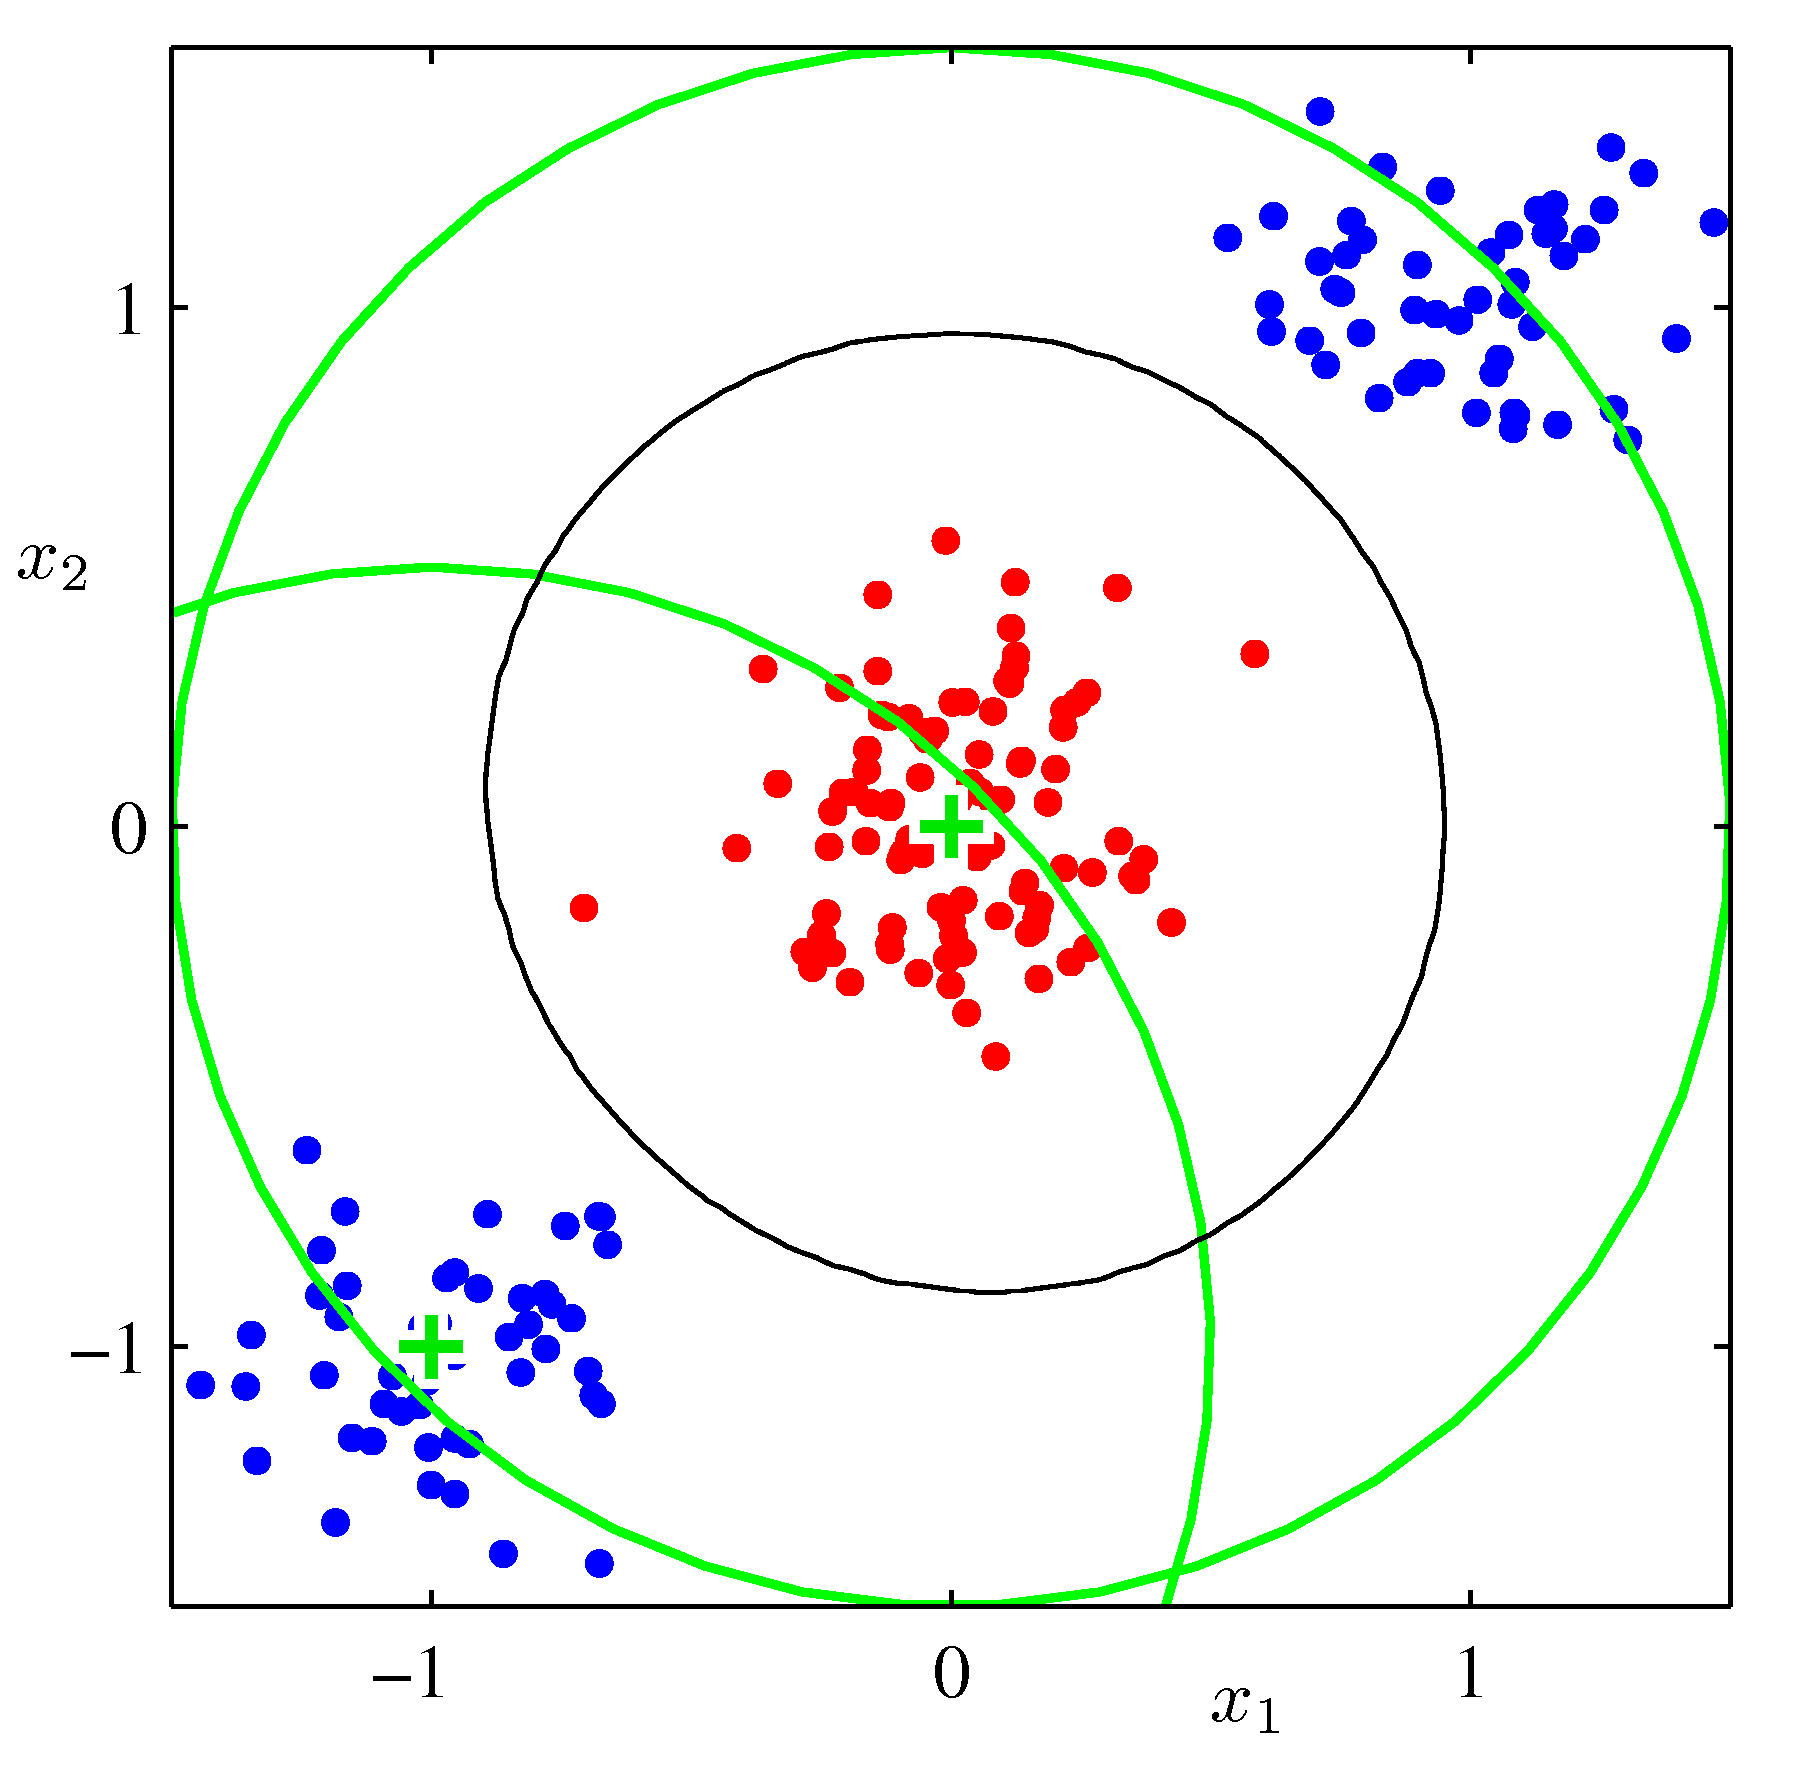
\includegraphics[scale=0.8]{Images/4-12a.png}
		\label{fig:4-12a}
		\end{minipage}
		\begin{minipage}[t]{0.5\linewidth}
		\centering
		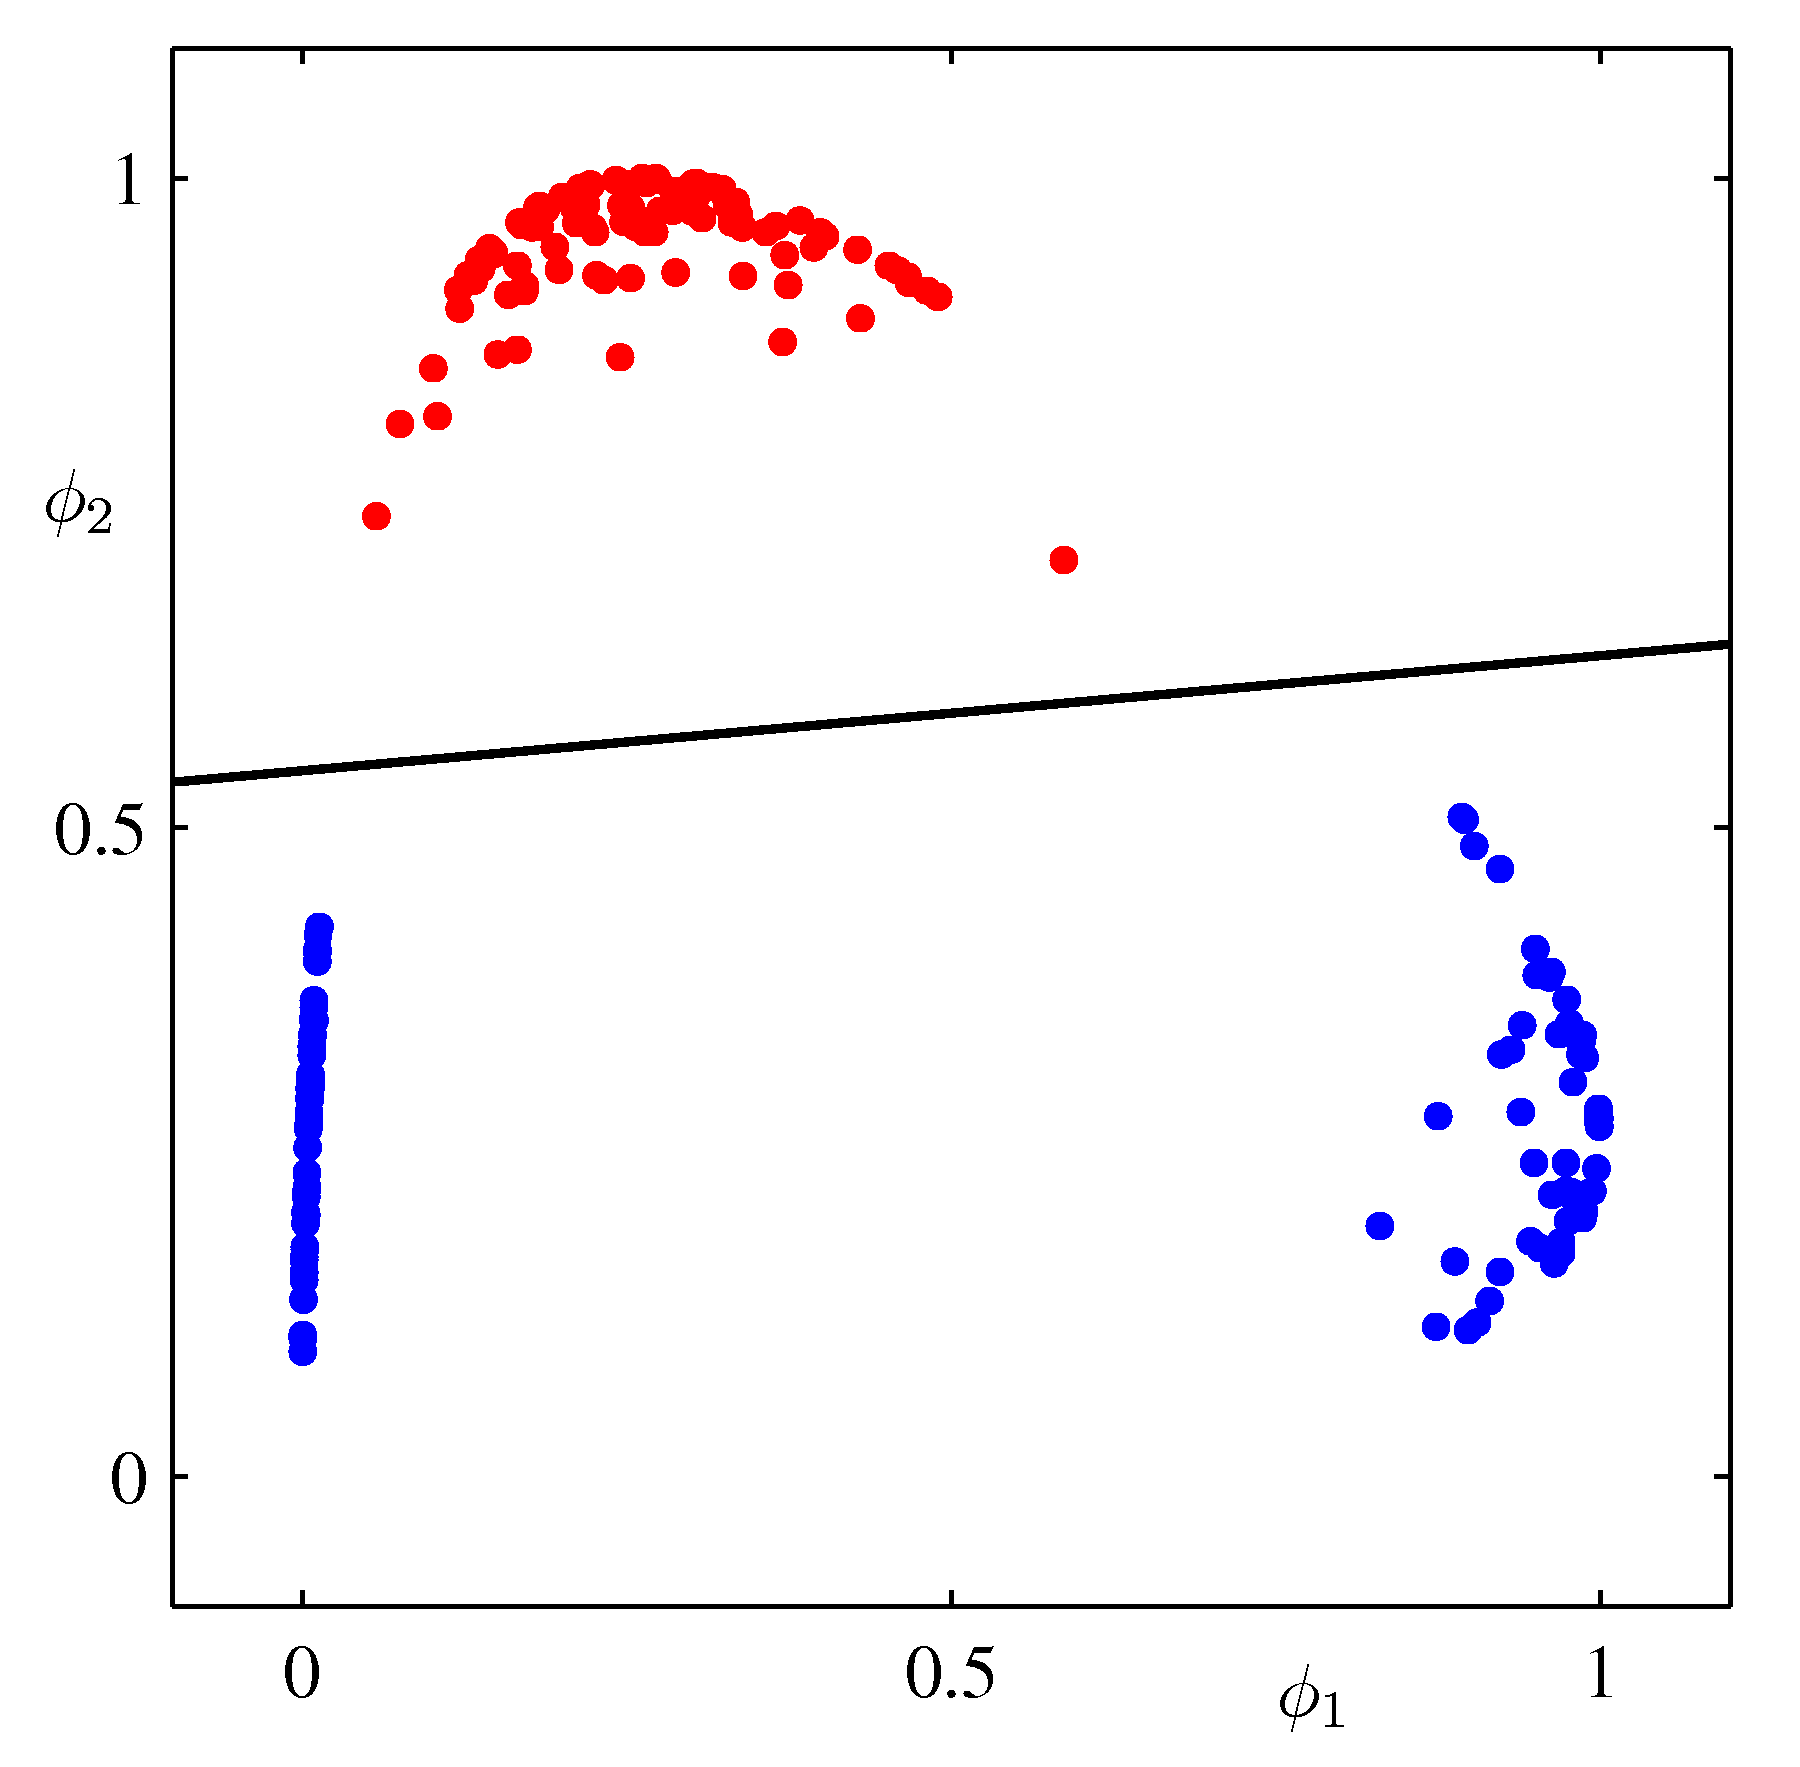
\includegraphics[scale=0.8]{Images/4-12b.png}
		\label{fig:4-12b}
		\end{minipage}
		\captionsetup{font={small}}
		\caption{非线性基底函数在线性分类模型中的应用。左图中展示了原始的输入空间$(x_1,x_2)$和两类数据(红色和蓝色)。同时在这个空间中定义了两个“高斯”基底函数$\phi_1(\bx)$和$\phi_2(\bx)$,其中心位于绿色的“+”,其轮廓为图中绿色的圆。右图中展示的是对应的特征空间$(\phi_1, \phi_2)$和利用logistic回归模型(详见第4.3.2节)确定的线性决策边界。这条决策边界在原始空间中对应的是一个非线性的决策边界,也就是左图中黑色的曲线。}
	\end{figure}
	\\
	\indent 在实际问题中,类别条件概率密度$p(\bx|\calC_k)$之间会存在明显的重叠,使得后验概率$p(\calC_k|\bx)$对于某些$\bx$并不能得到0或1的结果。在这样的情况下,可以对后验概率进行精确的建模,然后利用第1章中决策论的内容得到最优解。需要注意的是,非线性变换$\phi(\bx)$并不能解决类别重叠的问题,反而有可能使重叠的现象更加严重,甚至会在原始空间中没有出现重叠的地方搞出重叠来。不过,合适的非线性变换是可以简化后验概率建模的过程的。\\
	\indent 这样的固定基底函数有明显的局限性,在后面的章节中我们会使基底函数能够适应数据,从而解决这个问题。即使有这样那样的不足,固定基底函数模型仍然在实际应用中扮演了重要的角色,而且可以引出很多更加复杂的模型所需要的重要概念。
	}
	\subsection{logistic回归}
	\textnormal{一如既往,仍然从二分类问题入手来研究广义线性模型。通过在第4.2节中讨论的生成方法,在一般的假设条件下,类别$\calC_1$的后验概率可以写成以特征向量$\phi$为自变量的logistic sigmoid函数的形式,于是
	\begin{equation}
		p(\calC_1|\phi) = y(\phi) = \sigma(\bw^{\rmT}\phi)
	\end{equation}
	以及$p(\calC_2|\phi) = 1 - p(\calC_1|\phi)$。其中$\sigma(\cdot)$为logistic sigmoid函数,也就是(4.59)。在统计学中,这个模型称为logistic回归模型,尽管这是一个分类模型而非回归模型。\\
	\indent 对于$M$维的特征空间$\phi$,这个模型中含有$M$个参数。相比之下,如果利用高斯条件概率密度建模,然后用最大似然方法计算参数,那就需要确定$2M$个关于均值的参数和$M(M+1)/2$个关于协方差矩阵的参数。算上先验$p(\calC_1)$,足足要确定$M(M+5)/2+1$个参数,这个数量级可是$M$的平方,比logistic回归中要确定的参数数量多到不知道哪里去了。对于较大的$M$,直接利用logistic回归模型更是具有极大的优势。\\
	\indent 现在利用最大似然方法确定logistic回归模型中的参数。首先对logistic sigmoid函数求导,将结果表示为sigmoid函数自身的形式要更加简单:
	\begin{equation}
		\frac{\rmd \sigma}{\rmd a} = \sigma(1-\sigma)
	\end{equation}
	对于数据集$\{\phi_n, t_n\}$,其中$t_n \in \{0,1\}, \phi_n = \phi(\bx_n), n=1,...,N$,似然函数可以写成
	\begin{equation}
		p(\sft|\bw) = \prod_{n=1}^N y_n^{t_n} \{1-y_n\}^{1-t_n}
	\end{equation}
	其中$\sft = (t_1, ..., t_N)^{\rmT}$,$y_n = p(\calC_1|\phi_n)$。和往常一样,可以对似然函数求负对数然后将其定义为误差函数,实际上得到的是如下的交叉熵误差函数(cross-entropy error function):
	\begin{equation}
		E(\bw) = -\ln p(\sft|\bw) = -\sum_{n=1}^N \{t_n \ln y_n + (1-t_n)\ln (1-y_n)\}
	\end{equation}
	其中$y_n = \sigma(a_n), a_n = \bw^{\rmT}\phi_n$。对误差函数关于$\bw$求梯度,可以得到
	\begin{equation}
		\nabla E(\bw) = \sum_{n=1}^N (y_n - t_n)\phi_n
	\end{equation}
	其中利用了(4.88)。可以看出,关于logistic sigmoid导数的项都小时了,使得对数似然函数梯度的形式变得非常简单。特别地,某个数据$n$对梯度造成的影响是“误差”$(y_n - t_n)$(也就是目标值和模型预测值之间的差异)乘以基底函数向量$\phi_n$。此外,与(3.13)对比一下可以看出,这个梯度的形式与线性回归模型中的平方和误差函数的梯度具有相同的形式。\\
	\indent 如果需要的话,可以利用(4.91)得到顺序算法,其中的权重向量可以利用(3.22)进行更新,其中的$\nabla E_n$为(4.91)中的第$n$项。\\
	\indent 值得注意的是,对于线性可分的数据集,最大似然方法可能会产生严重的过拟合现象。这是因为最大似然解所对应的是$\sigma = 0.5$的超平面,也就是$\bw^{\rmT}\phi=0$的情况,从而将两个类别分开,而且$\bw$的大小趋近于无限大。在这种情况下,logistic sigmoid函数在特征空间中会变得无比陡峭,形成一个跳变的阶梯函数,所以每个类别$k$中的数据都会得到$p(\calC_k|\bx)=1$的后验概率。此外,通常来讲,这些解之间是存在连续性的,因为任何的分割超平面都会对训练数据给出相同的后验概率,如图10.13所示。最大似然方法无法区分解的优劣,而且具体得到哪个解,要取决于优化的方法和初始参数的选择。需要注意的是,只要数据集是线性可分的,那么即使数据点的数量比模型中参数的数量大很多,也很容易出现过拟合的问题。通过引入先验并计算$\bw$的最大后验概率解,或者等价地在误差函数中添加正则项,可以避免这个问题。
	}
	\subsection{迭代重加权最小二乘法}
	\textnormal{在第3章中讨论线性回归模型时,假设噪声为高斯模型条件下的最大似然解是可以得到闭式解的。这是由于对数似然函数是参数向量$\bw$的二次函数。对于logistic回归而言,闭式解就不复存在了,因为logistic sigmoid函数是非线性函数。不过这个影响不是很大,因为误差函数是凸函数,所以具有唯一的最小值。此外,误差函数可以使用基于Newton-Raphson优化的迭代计算方式求取对数似然函数的局部二次近似。对于最小化目标函数$E(\bw)$,Newton-Raphson更新的形式为(Fletcher, 1987; Bishop and Nabney, 2008)
	\begin{equation}
		\bw^{(\mathrm{new})} = \bw^{(\mathrm{old})} - \mathbf{H}^{-1} \nabla E(\bw)
	\end{equation}
	其中$\mathbf{H}$为Hessian矩阵,其元素是$E(\bw)$关于$\bw$各个分量的二阶导数。\\
	\textcolor{red}{【译者注:求取Hessian矩阵的公式为:】
	\begin{equation*}
		\mathbf{H} = \left[\begin{matrix}
			\frac{\partial^2f}{\partial x_1^2} & \frac{\partial^2f}{\partial x_1 \partial x_2} & \cdots & \frac{\partial^2f}{\partial x_1 \partial x_n}\\
			\frac{\partial^2f}{\partial x_2 \partial x_1} & \frac{\partial^2f}{\partial x^2_2} & \cdots & \frac{\partial^2f}{\partial x_2 \partial x_n}\\
			\vdots & \vdots & \ddots & \vdots \\
			\frac{\partial^2f}{\partial x_n \partial x_1} & \frac{\partial^2f}{\partial x_n \partial x_2} & \cdots & \frac{\partial^2f}{\partial x^2_n}
		\end{matrix}\right]
	\end{equation*}}
	\indent 首先对线性回归模型(3.3)的平方和误差函数(3.12)使用Newton-Raphson方法。该误差函数的梯度和Hessian矩阵为
	\begin{align}
		\nabla E(\bw) &= \sum_{n=1}^N (\bw^{\rmT}\bfphi_n - t_n)\bfphi_n = \bfPhi^{\rmT}\bfPhi \bw - \bfPhi^{\rmT} \sft \\
		\mathbf{H} = \nabla \nabla E(\bw) &= \sum_{n=1}^N \bfphi_n \bfphi_n^{\rmT} = \bfPhi^{\rmT} \bfPhi
	\end{align}
	其中$\bfPhi$为$N \times M$维的设计矩阵,其第$n$行为$\bfphi_n^{\rmT}$。那么Newton-Raphson更新的形式可以写成
	\begin{equation}
	\begin{split}
		\bw^{\mathrm{(new)}} &= \bw^{\mathrm{(old)}} - \left(\bfPhi^{\rmT} \bfPhi \right)^{-1} \left\{\bfPhi^{\rmT}\bfPhi\bw^{\mathrm{(old)}} - \bfPhi^{\rmT}\sft\right\}\\
		&= \left(\bfPhi^{\rmT}\bfPhi\right)^{-1} \bfPhi^{\rmT} \sft
	\end{split}
	\end{equation}
	这正是标准的最小二乘解。需要注意的是,此时的误差函数是二次函数,所以Newton-Raphson公式可以给出每一步的确切解。\\
	\indent 接下来对logistic回归模型的交叉熵误差函数(4.90)使用Newton-Raphson方法。根据(4.91),该误差函数的梯度和Hessian矩阵为
	\begin{align}
		\nabla E(\bw) &= \sum_{n=1}^N (y_n - t_n)\bfphi_n = \bfPhi^{\rmT}(\sfy - \sft)\\
		\mathbf{H} &= \nabla \nabla E(\bw) = \sum_{n=1}^N y_n (1-y_n)\bfphi_n \bfphi_n^{\rmT} = \bfPhi^{\rmT} \mathbf{R} \bfPhi
	\end{align}
	其中利用了公式(4.88)。另外还引入了$N \times N$维的对角矩阵$\mathbf{R}$,其对角元素为
	\begin{equation}
		R_{nn} = y_n(1 - y_n)
	\end{equation}
	可以看出,Hessian矩阵不再是一个常数了,而是通过权重矩阵$\mathbf{R}$与$\bw$扯上了关系,于是乎误差函数也不再是一个二次函数了。根据logistic sigmoid函数的形式,有$0 < y_n <1$,所以对于任意的向量$\mathbf{u}$都有$\mathbf{u}^{\rmT}\mathbf{H}\mathbf{u} > 0$,所以Hessian矩阵$\mathbf{H}$是正定的。这表明误差函数是一个关于$\bw$的凸函数,所以是有唯一最小值的。\\
	\indent 于是,logistic回归模型的Newton-Raphson更新公式可以写成
	\begin{equation}
	\begin{split}
		\bw^{(\mathrm{new})} &= \bw^{(\mathrm{old})} - (\bfPhi^{\rmT} \mathbf{R} \bfPhi)^{-1}\bfPhi^{\rmT}(\sfy - \sft)\\
		&= (\bfPhi^{\rmT} \mathbf{R} \bfPhi)^{-1} \left\{\bfPhi^{\rmT} \mathbf{R} \bfPhi \bw^{(\mathrm{old})} - \bfPhi^{\rmT} (\sfy - \sft)\right\} \\
		&= (\bfPhi^{\rmT} \mathbf{R} \bfPhi)^{-1} \bfPhi^{\rmT}\mathbf{R}\boldsymbol{\mathsf{z}}
	\end{split}
	\end{equation}
	其中$\boldsymbol{\mathsf{z}}$为$N$维向量,其元素为
	\begin{equation}
		\boldsymbol{\mathsf{z}} = \bfPhi \bw^{(\mathrm{old})} - \mathbf{R}^{-1}(\sfy - \sft)
	\end{equation}
	可以看出,更新公式(4.99)其实是一个加权最小二乘问题中的一堆正规方程构成的集合。由于权重矩阵$\mathbf{R}$依赖于参数向量$\bw$而非常数,所以必须要迭代使用正规方程,每次迭代都利用新的权重向量$\bw$计算新的权重矩阵$\mathbf{R}$。所以这个算法称为迭代重加权最小二乘法(iterative reweighted least squares, IRLS, Rubin, 1983)。与加权最小二乘问题一样,对角权重矩阵$\mathbf{R}$的元素可以看成是变量,因为logistic回归模型中的$t$的均值和方差为
	\begin{align}
		\mathbb{E}[t] &= \sigma{\bx} =y \\
		\mathrm{var}[t] &= \mathbb{E}[t^2] - \mathbb{E}[t]^2 = \sigma(\bx) - \sigma(\bx)^2 = y(1 - y)
	\end{align}
	其中利用了当$t \in \{0,1\}$时$t^2 = t$的性质。实际上,我们可以将IRLS看成是变量$a = \bw^{\rmT}\bfphi$空间中线性问题的解。$\sfz$中的第$n$个元素$z_n$可以看成是在这个空间中,通过对logistic sigmoid函数在$\bw^{(\mathrm{old})}$附近进行局部线性近似得到的目标值:
	\begin{equation}
	\begin{split}
		a_n(\bw) &\approx a_n (\bw^{(\mathrm{old})}) + \frac{\rmd a_n}{\rmd y_n}\bigg|_{\bw^{(\mathrm{old})}} (t_n - y_n) \\
		&= \bfphi^{\rmT} \bw^{(\mathrm{old})} - \frac{(y_n - t_n)}{y_n(1-y_n)} = z_n
	\end{split}
	\end{equation}
	}
	\subsection{多分类logistic回归}
	\textnormal{在讨论多分类问题的生成模型时。我们已经看到,对于一类分布而言,后验概率是由特征变量线性函数的softmax变换得到的,于是
	\begin{equation}
		p(\calC_k | \bfphi) = y_k(\bfphi) = \frac{\exp (a_k)}{\sum_j \exp (a_j)}
	\end{equation}
	其中的“激励”【我怎么知道会用到自动控制原理的名词。。。】$a_k$为
	\begin{equation}
		a_k = \bw^{\rmT}_k \bfphi
	\end{equation}
	在这里我们利用最大似然方法来分别确定类别条件概率密度和类别先验,然后利用贝叶斯定理求取相应的后验概率,从而确定参数$\{\bw_k\}$。不过现在,我们可以直接利用最大似然方法确定模型参数$\{\bw_k\}$。首先要做的第一件事是将$y_k$关于所有的激励$a_j$求偏导,于是
	\begin{equation}
		\frac{\partial y_k}{\partial a_j} = y_k (I_{kj} - y_j)
	\end{equation}
	其中$I_{kj}$为单位矩阵的元素。\\
	\indent 然后写出似然函数。在这个问题中采用1-of-K编码是最方便的,于是似然函数为
	\begin{equation}
		p(\mathbf{T}|\bw_1, ..., \bw_K) = \prod_{n=1}^N \prod_{k=1}^K p(\calC_k|\bfphi_n)^{t_{nk}} = \prod_{n=1}^N \prod_{k=1}^K y_{nk}^{t_{nk}}
	\end{equation}
	其中$y_{nk} = y_k(\bfphi_n)$。$\mathbf{T}$是$N \times K$维的矩阵,其元素$t_{nk}$为目标变量。对这个函数取负对数,
	\begin{equation}
		E(\bw_1, ..., \bw_K) = -\ln p(\mathbf{T}|\bw_1, ..., \bw_K) = -\sum_{n=1}^N \sum_{k=1}^K t_{nk} \ln y_{nk}
	\end{equation}
	这就是多分类问题的交叉熵误差函数。\\
	\indent 现在将误差函数关于其中一个参数向量$\bw_j$求梯度。利用(4.106)中softmax函数求导的结果,可以得到
	\begin{equation}
		\nabla_{\bw_j}E(\bw_1, ..., \bw_K) = \sum_{n=1}^N (y_{nj} - t_{nj})\bfphi_n
	\end{equation}
	其中用到了$\sum_k t_{nk} = 1$的性质。此刻涛声依旧【拖走】,我们所得到的梯度与线性模型的平方和误差函数、logistic回归模型的交叉熵误差函数具有相同的形式,即误差$(y_{nj} - t_{nj})$与基底函数$\bfphi_n$的乘积。再次涛声依旧【再拖走】,我们可以利用这个公式来构建顺序算法,仍然利用(3.22)来更新权重向量。\\
	\indent 很明显,线性回归模型在数据点$n$处关于参数向量$\bw$的对数似然函数的形式为“误差”$y_n -t_n$乘以特征向量$\bfphi_n$。类似地,对于logistic sigmoid激活函数和它的交叉熵误差函数(4.90),以及softmax激活函数和它的多分类交叉熵误差函数(4.108)都具有类似的形式。它们都是一个更加一般的结果的特殊情况,我们会在第4.3.6节中看到这个内容。\\
	\indent 为了求出可以批量处理的算法,我们再次利用Newton-Raphson更新来确定多分类问题的IRLS算法。这需要求一个$M \times M$维的Hessian矩阵,其位于$(j,k)$位置的元素为
	\begin{equation}
		\nabla_{\bw_k} \nabla_{\bw_j} E(\bw_1, ..., \bw_K) = -\sum_{n=1}^N y_{nk} (I_{kj} - y_{nj}) \bfphi_n \bfphi_n^{\rmT}
	\end{equation}
	和二分类问题一样,多分类logistic回归模型的Hessian矩阵是正定的,所以误差函数同样是具有唯一最小值的。多分类问题中IRLS实际应用的相关细节可以在参考文献Bishop and Nabney(2008)中找到。
	}
	\subsection{probit回归}
	\textnormal{我们已经看到,在指数分布族这个广泛的类别条件概率分布范围中,最后得到的后验概率是特征变量线性函数的logistic变换(或者softmax变换)。不过,并不是所有的类别条件概率密度都会得到这么简单的后验概率(比如高斯混合模型)。所以寻找其他类型的概率判别模型或许是更好的选择。在本节中,我们会回到二分类问题的研究中,以及重新回到广义线性模型的基本框架,即
	\begin{equation}
		p(t = 1 | a) = f(a)
	\end{equation}
	其中$a = \bw^{\rmT} \bfphi$,$f(\cdot)$为激活函数。\\
	\indent 确定联系函数的一种方式是通过噪声阈值模型。对于任意的输入$\bfphi_n$,令$a_n = \bw^{\rmT} \bfphi_n$,并将目标值设置为
	\begin{equation}
		\left\{\begin{matrix}
			t_n = 1 & \mathrm{if}\ a_n \geqslant \theta \\
			t_n = 0 & \mathrm{otherwise}
		\end{matrix} \right.
	\end{equation}
	如果$\theta$的值来自于概率密度$p(\theta)$,那么相应的激活函数将是一个分布函数
	\begin{equation}
		f(a) = \int_{-\infty}^a p(\theta) \rmd \theta
	\end{equation}
	如图4.13所示。
	\begin{figure}[ht]
		\centering
		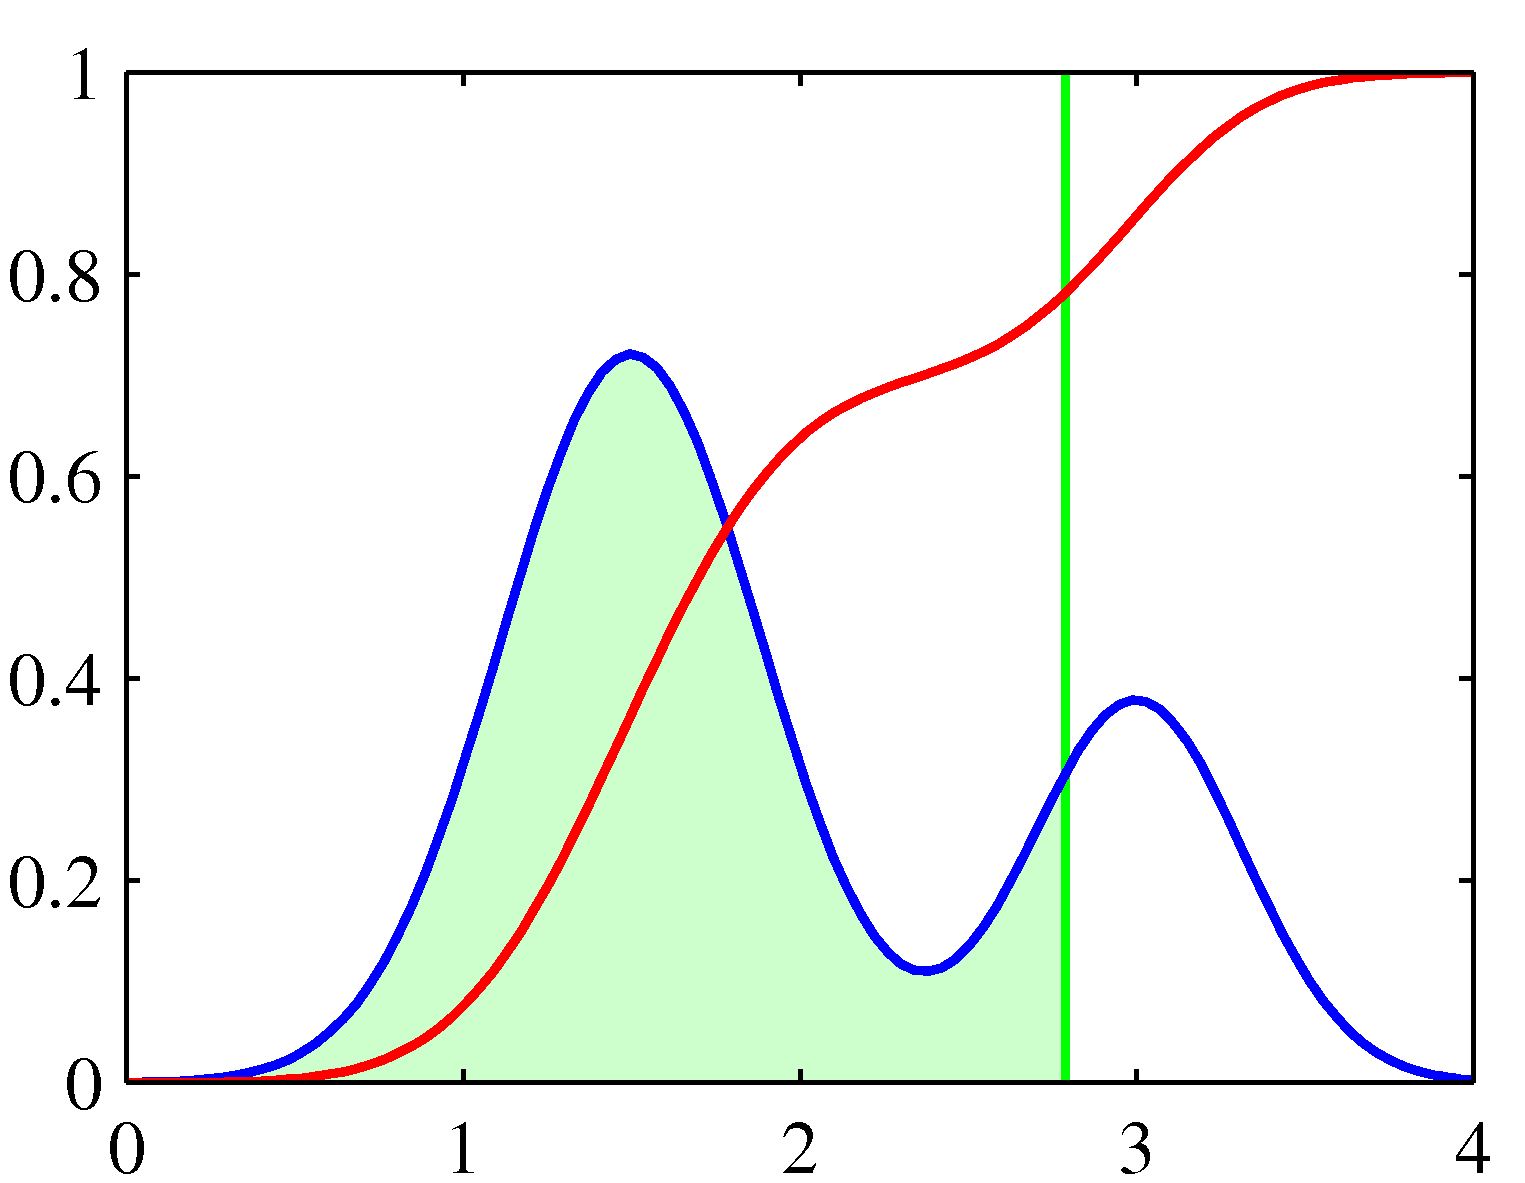
\includegraphics[scale=0.8]{Images/4-13.png}
		\label{fig:4-13}
		\captionsetup{font={small}}
		\caption{概率密度函数$p(\theta)$如图中的蓝色曲线所示,该概率密度是一个高斯混合模型,包含有2个分量。图中的红色曲线为概率分布函数。其中,蓝色曲线对应的函数值(例如垂直绿色直线处)是该点处红色曲线的斜率,而红色曲线对应的函数值则等于蓝色曲线下方绿色阴影部分的面积。在随机阈值模型中,如果$a = \bw^{\rmT} \bfphi$的值超过阈值则将类别标签标记为$t = 1$,否则$t = 0$。这与分布函数$f(a)$给出的激活函数是等价的。}
	\end{figure}
	\\
	\indent 举一个特殊的例子,假设概率密度$p(\theta)$是均值为0、方差为1的高斯分布。于是相应的概率分布函数为
	\begin{equation}
		\Phi(a) = \int_{-\infty}^a \mathcal{N}(\theta | 0,1)\rmd \theta
	\end{equation}
	这就是逆probit函数。它与logistic sigmoid函数相似,都是S型的,其图像如图4.9所示。需要注意的是,即使使用不这么特殊的高斯分布,也不会对这个模型造成影响,因为它对应的是一个经过缩放的线性系数$\bw$。许多用于计算这个函数的数值计算包都与下面的这个函数紧密相关:
	\begin{equation}
		\mathrm{erf}(a) = \frac{2}{\sqrt{\pi}}\int_0 ^a \exp(-\theta^2/2)\rmd \theta
	\end{equation}
	这个函数称为erf函数或者error函数(与误差函数不是一个东西哈)。它对应的逆profit函数为
	\begin{equation}
		\Phi(a) = \frac{1}{2}\left\{1 + \frac{1}{\sqrt{2}}\mathrm{erf}(a)\right\}
	\end{equation}
	基于profit激活函数的广义线性模型称为逆probit回归模型。\\
	\indent 我们可以通过最大似然方法来确定这个模型的参数。在实际应用中,利用probit回归得到的结果与logistic回归类似,不过我们会在第4.5节中看到,在研究贝叶斯观点下的logistic回归时,probit模型还有另外的一些用途。\\
	\indent 在实际应用中,异常值是一个很大的问题,在输入向量$\bx$的检测出现错误,或者目标值$t$的标注出现错误时,都会出现异常值。由于这样的数据会对决策边界产生严重的不利影响,所以对分类器的影响也是相当恶劣的。需要注意的是,logistic回归模型和probit回归模型在这个问题上的表现很是不同,因为当$x \rightarrow \infty$时,logistic sigmoid函数的衰减是$\exp(-x)$量级的,而probit激活函数则是$\exp(-x^2)$,所以probit模型对异常值更加敏感。\\
	\indent 不过,logistic模型和probit模型都建立在同一个假定之上,即直接利用了数据的标签。这样一来,错误标定会很容易对概率模型造成影响。在这里假设误分类的概率为$\epsilon$(Opper and Winther, 2000a),那么数据$\bx$相应目标值的分布为
	\begin{equation}
	\begin{split}
		p(t|\bx) &= (1 - \epsilon) \sigma(\bx) + \sigma(1 - \sigma(\bx)) \\
		&= \epsilon + (1 - 2\epsilon)\sigma(\bx)
	\end{split}
	\end{equation}
	其中$\sigma(\bx)$为输入向量$\bx$的激活函数。其中$\epsilon$的值可以提前设定,也可以当成一个超参数从数据中推断得到。
	}
	\subsection{标准联系函数}
	\textnormal{对于带有高斯噪声的线性回归模型,其负对数似然函数的误差函数为(3.12)、如果我们将某一数据点$n$对误差函数造成的影响(即数据点$n$对应的那个分量)关于参数向量$\bw$求导,得到的是$y_n -t_n$乘以特征向量$\bfphi_n$这样形式的结果,其中$y_n = \bw^{\rmT}\bfphi_n$。类似地,对于logistic sigmoid激活函数和它的交叉熵误差函数(4.90),以及softmax激活函数和它的多分类交叉熵误差函数(4.108)都具有类似的形式。现在我们证明一下这都来自于一个一般的结果,即假设目标变量的条件分布来自于指数型分布族,并选取了名为标准联系函数(canonical link function)的激活函数后所得到的一般性结果。\\
	\indent 再次利用指数型分布族的约束形式(4.84),不过需要注意一个问题,我们现在是假设目标变量$t$的分布属于指数型分布族,而不是第4.2.4节里那样对输入变量$\bx$的分布进行假设。于是可以写出目标变量的条件分布
	\begin{equation}
		p(t|\eta, s) = \frac{1}{s}h\left(\frac{t}{s}\right)g(\eta)\exp \left\{\frac{\eta t}{s}\right\}
	\end{equation}
	利用与(2.226)相同的推导方法,可以得到$t$的条件均值$y$为
	\begin{equation}
		y \equiv \mathbb{E}[t|\eta] = -s \frac{\rmd}{\rmd \eta} \ln g(\eta)
	\end{equation}
	所以$y$与$\eta$一定是相关的,我们将这个关系表示为$\eta = \psi(y)$。\\
	\indent 根据参考文献Nelder and Wedderburn(1972),我们可以定义广义线性模型为,$y$是经过线性变换的输入变量(或特征)的非线性函数,即
	\begin{equation}
		y = f(\bw^{\rmT} \bfphi)
	\end{equation}
	其中$f(\cdot)$为激活函数,而$f^{-1}(\cdot)$则是统计学中的联系函数。\\
	\indent 现在我们研究这个模型关于$\eta$的对数似然函数,
	\begin{equation}
		\ln p(\sft|\eta, s) = \sum_{n=1}^N \ln p(t_n|\eta,s) = \sum_{n=1}^N \left\{\ln g(\eta_n) + \frac{\eta_n t_n}{s}\right\} + \mathrm{const}
	\end{equation}
	其中我们做出了一个假设,即所有的观测都有共同的放缩系数(举个例子,比如高斯分布中的噪声方差),所以$s$与$n$是相互独立的。对数似然函数关于模型参数$\bw$的导数为
	\begin{equation}
	\begin{split}
		\nabla_{\bw} \ln p(\sft|\eta,s) &= \sum_{n=1}^N \left\{\frac{\rmd}{\rmd \eta_n} \ln g(\eta_n) + \frac{t_n}{s}\right\} \frac{\rmd \eta_n}{\rmd y_n} \frac{\rmd y_n}{\rmd a_n} \nabla a_n \\
		&= \sum_{n=1}^N \frac{1}{s} {t_n - y_n} \psi'(y_n)f'(a_n)\bfphi_n
	\end{split}
	\end{equation}
	其中$a_n = \bw^{\rmT} \bfphi_n$,$y_n = f(a_n)$,另外用到了(4.119)中关于$\mathbb{E}[t|\eta]$的结论。现在可以看出,如果我们选取一个特殊形式的联系函数
	\begin{equation}
		f^{-1}(y) = \psi(y)
	\end{equation}
	那么这个公式将大幅简化,因为此时$f(\psi(y)) = y$,所以$f'(\psi)\psi'(y) = 1$。另外,由于$a = f^{-1}(y)$,所以$a = \psi$,于是$f'(a) \psi'(y) = 1$。在这个情况下,误差函数的梯度就退化为
	\begin{equation}
		\nabla E(\bw) = \frac{1}{s} \sum_{n=1}^N \{y_n - t_n\}\bfphi_n
	\end{equation}
	对于高斯分布,$s = \beta^{-1}$,对于logistic模型,$s = 1$。
	}
	\section{Laplace近似}
	\insertline
	\textnormal{
	\indent 在第4.5节中我们会研究贝叶斯视角下的logistic回归。我们会看到这个过程比第3.3节和第3.5节中贝叶斯视角下的线性回归模型复杂得多。特别地,我们不能关于参数向量$\bw$求积分,因为后验分布在这里就不是高斯分布了。所以我们需要引入一些近似。在本书后面的一些章节中,我们会专门研究分析近似和数值抽样的相关方法。\\
	\indent 现在我们先使用一个比较简单但应用很广泛的方法,Laplace近似。Laplace近似的目的,是将某连续变量的概率密度近似成高斯分布。首先研究一元连续变量$z$的情况,并假设$p(z)$为
	\begin{equation}
		p(z) = \frac{1}{Z} f(z)
	\end{equation}
	其中$Z = \int f(z) \rmd z$为归一化常数,在这里我们假设$Z$的值是未知的。在Laplace近似中,我们要求出一个中心位于分布$p(z)$的模处的高斯近似$q(z)$。第一步当然是求出$p(z)$的模,也就是使得$p'(z_0) = 0$的$z_0$,或者是
	\begin{equation}
		\frac{\rmd f(z)}{\rmd z}\bigg|_{z=z_0}=0
	\end{equation}
	\indent 高斯分布具有一个性质,其对数是一个关于变量的二次函数。所以我们将$\ln f(z)$在模$z_0$处进行Taylor展开,于是
	\begin{equation}
		\ln f(z) \approx \ln f(z_0) - \frac{1}{2}A(z - z_0)^2
	\end{equation}
	其中
	\begin{equation}
		A = - \frac{\rmd ^2}{\rmd z^2}\ln f(z) \bigg|_{z=z_0}
	\end{equation}
	需要注意的是,Taylot展开式中的一阶项并没有消失,因为$z_0$是这个分布的一个局部最大值。对等式两侧同时取指数,
	\begin{equation}
		f(z) \approx f(z_0) \exp\left\{-\frac{A}{2}(z - z_0)^2\right\}
	\end{equation}
	于是可以利用归一化高斯分布的标准形式确定归一化分布$q(z)$了,即
	\begin{equation}
		q(z) = \left(\frac{A}{2\pi}\right)^{1/2}\exp\left\{-\frac{A}{2}(z - z_0)^2\right\}
	\end{equation}
	Laplace近似的图像如图4.14所示。需要注意的是,仅在精度$A>0$时,高斯近似的表现才会比较良好,也就是说,驻点$z_0$必须是局部最大值才行,因为只有这样$f(z)$在$z_0$处的二阶导数才是负的。
	\begin{figure}[ht]
		\begin{minipage}[t]{0.5\linewidth}
		\centering
		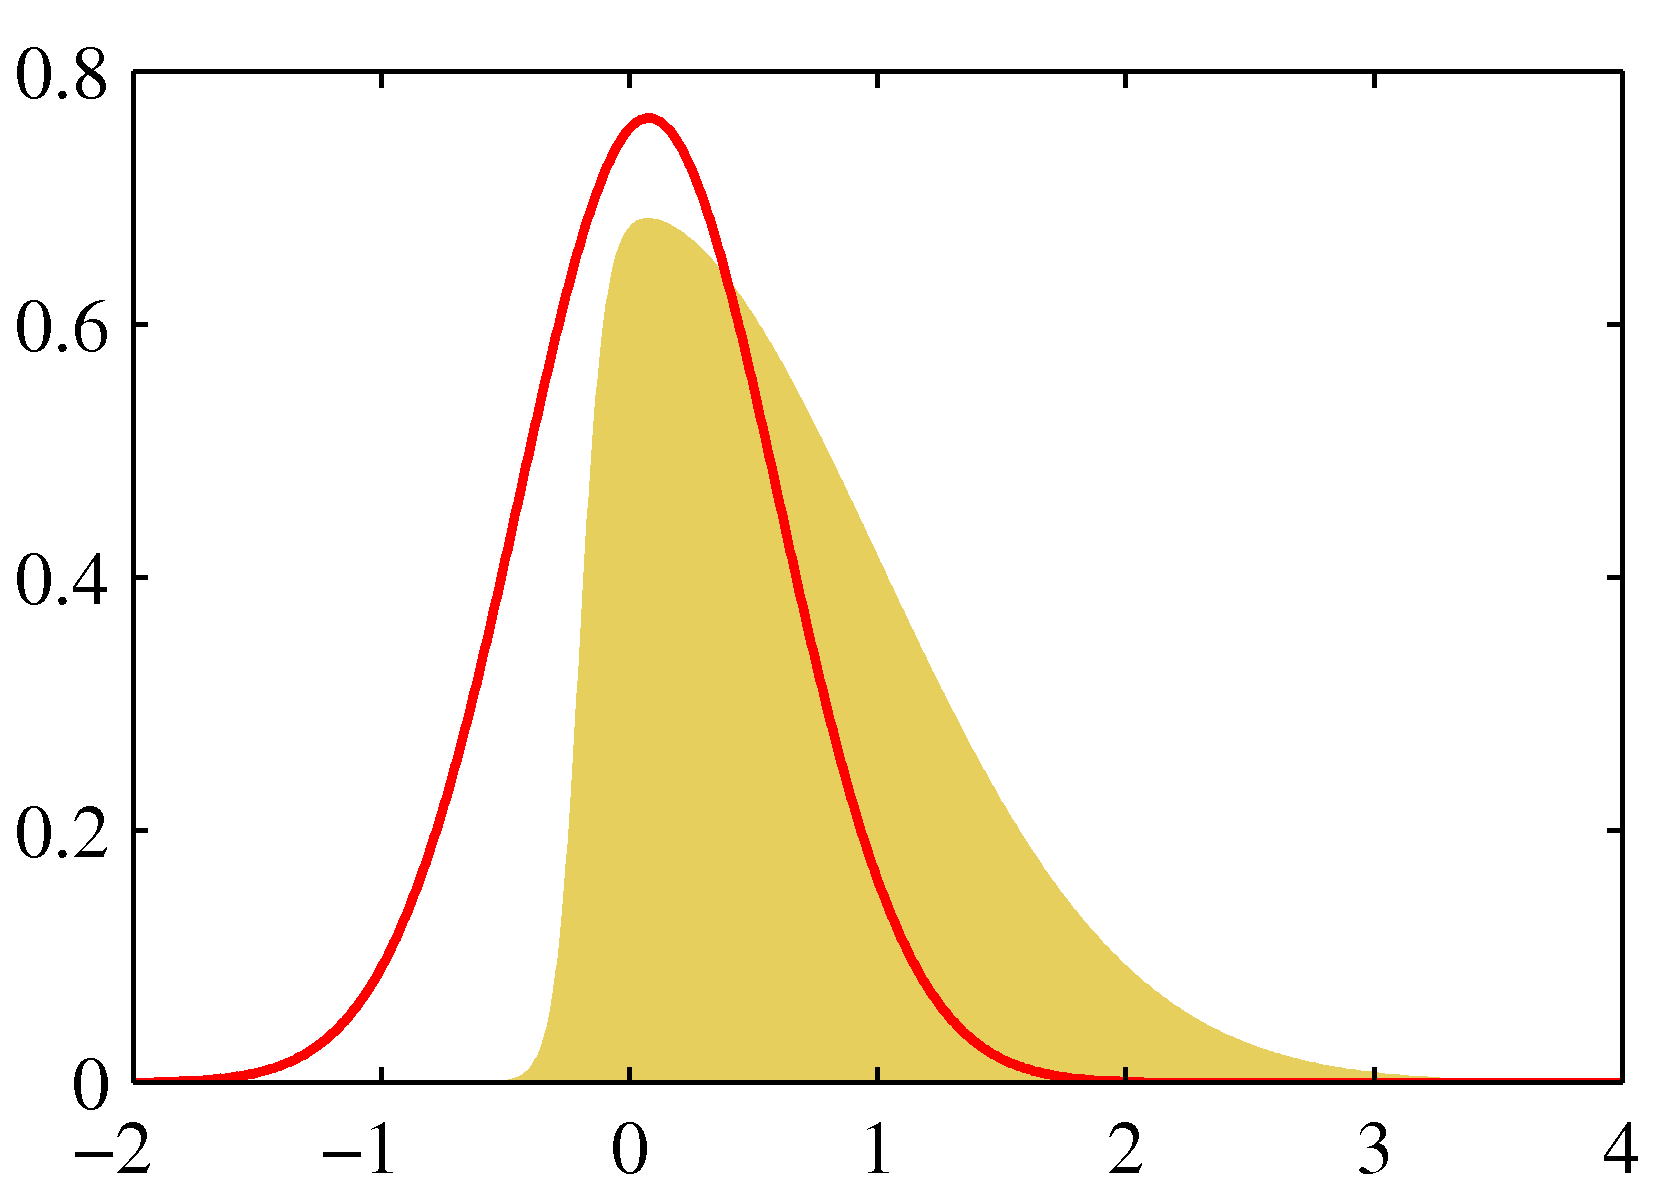
\includegraphics[scale=0.8]{Images/4-14a.png}
		\label{fig:4-14a}
		\end{minipage}
		\begin{minipage}[t]{0.5\linewidth}
		\centering
		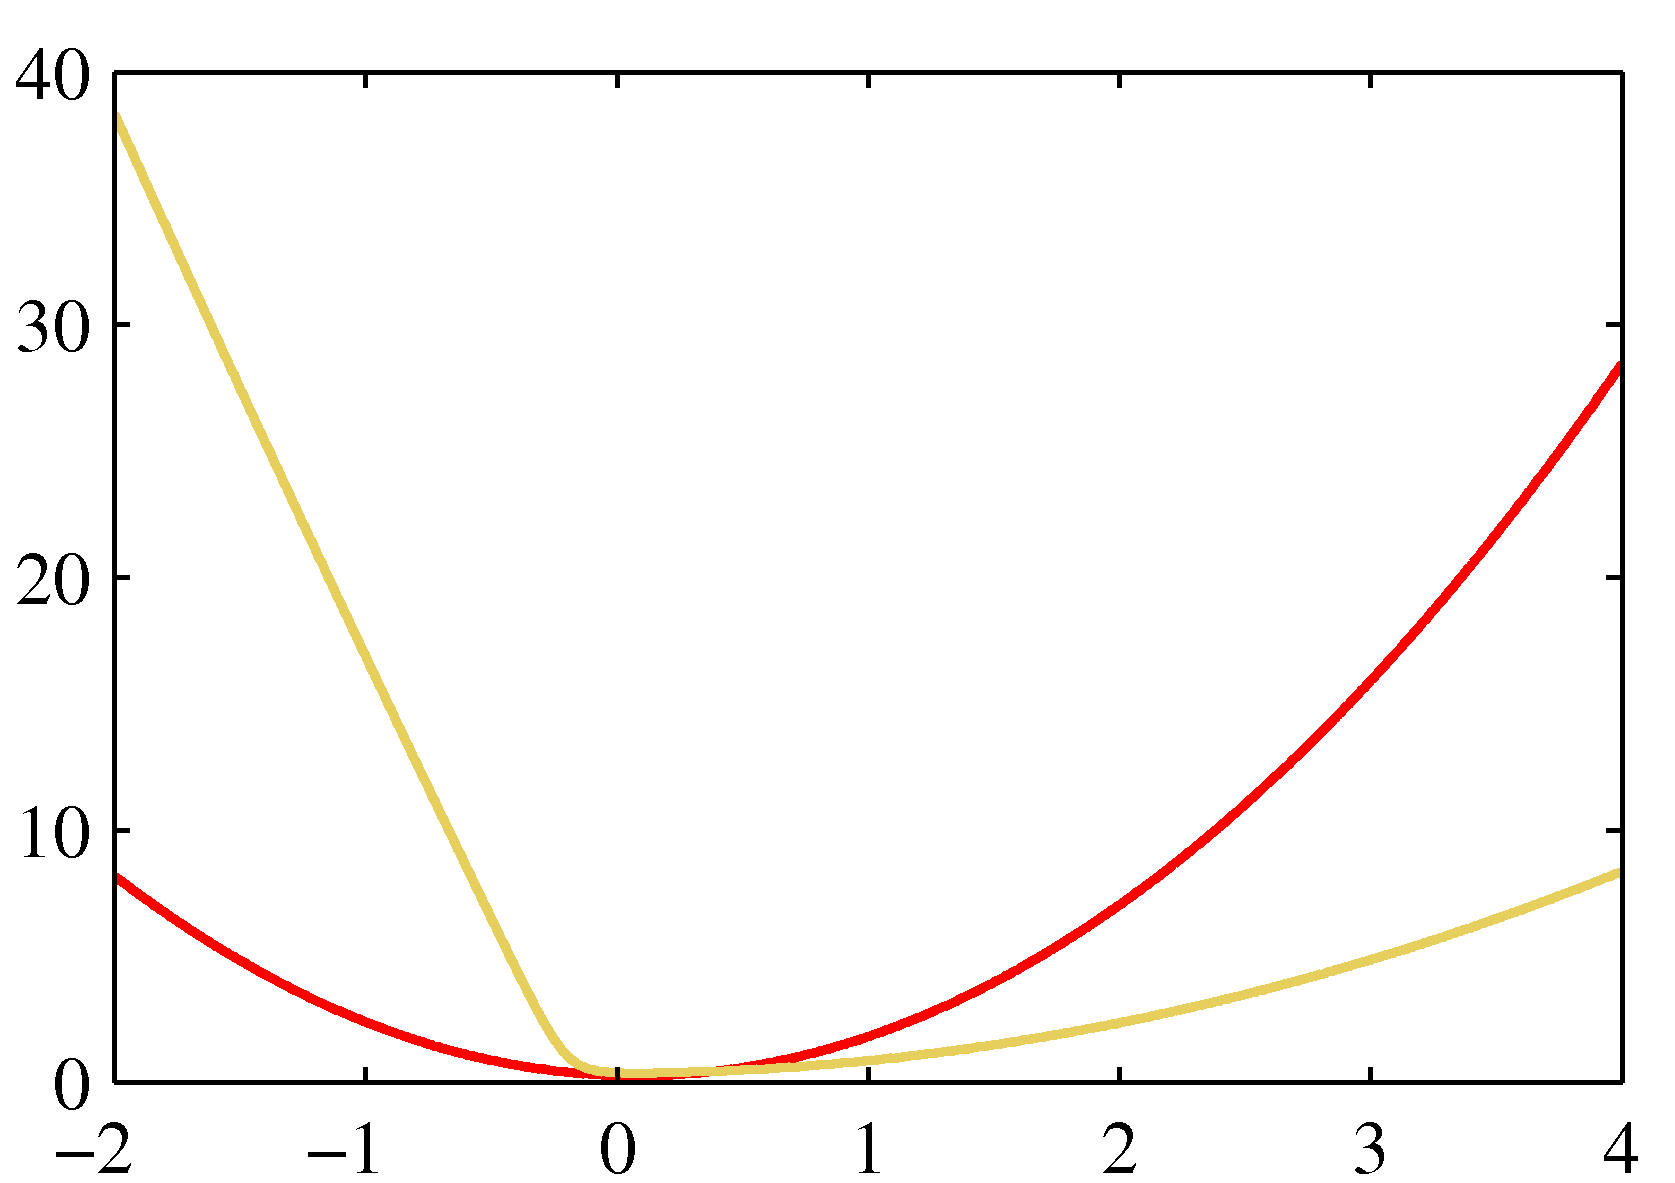
\includegraphics[scale=0.8]{Images/4-14b.png}
		\label{fig:4-14b}
		\end{minipage}
		\captionsetup{font={small}}
		\caption{对分布$p(z) \propto \exp(-z^2/2)\sigma(20z+4)$进行Laplace近似的结果,其中$\sigma(z)=(1+e^{-z})^{-1}$为logistic sigmoid函数。左图中展示的是经过归一化的分布$p(z)$(黄色)和中心位于$p(z)$的模$z_0$处的Laplace近似(红色)。右图中展示的是相应的负对数曲线。}
	\end{figure}
	\\
	\indent 我们可以将Laplace近似扩展到$M$维空间$\mathbf{z}$中,对分布$p(\mathbf{z}) = f(\mathbf{z})/Z $进行近似。在驻点$\mathbf{z}_0$处,梯度$\nabla f(\mathbf{z}) = 0$。在驻点附近进行Taylor展开,
	\begin{equation}
		\ln f(\mathbf{z}) \approx \ln f(\mathbf{z}_0) - \frac{1}{2} (\mathbf{z} - \mathbf{z}_0)^{\rmT} \mathbf{A} (\mathbf{z} - \mathbf{z}_0)
	\end{equation}
	其中$\mathbf{A}$为$M \times M$维的Hessian矩阵,
	\begin{equation}
		\mathbf{A} = -\nabla \nabla \ln f(\mathbf{z})|_{\mathbf{z} = \mathbf{z}_0}
	\end{equation}
	其中$\nabla$为梯度计算符。\\
	\indent 对等式两侧同时取指数,
	\begin{equation}
		f(\mathbf{z}) \approx f(\mathbf{z}_0)\exp \left\{-\frac{1}{2}(\mathbf{z} - \mathbf{z}_0)^{\rmT}\mathbf{A}(\mathbf{z} - \mathbf{z}_0)\right\}
	\end{equation}
	分布$q(\mathbf{z})$是与$f(\mathbf{z})$成正比的,归一化系数可以从经过归一化的多元高斯分布标准形式(2.43)得到,即
	\begin{equation}
		q(\mathbf{z}) = \frac{|\mathbf{A}|^{1/2}}{(2 \pi)^{M/2}}\exp \left\{-\frac{1}{2}(\mathbf{z}-\mathbf{z}_0)^{\rmT}\mathbf{A}(\mathbf{z}-\mathbf{z}_0)\right\} = \calN(\mathbf{z}|\mathbf{z}_0, \mathbf{A}^{-1})
	\end{equation}
	其中$|\mathbf{A}|$表示$\mathbf{A}$的行列式。当精度矩阵$\mathbf{A}$为正定矩阵时,高斯分布将具备完备的定义,也就是要求驻点$\mathbf{z}_0$是局部最大值,不可以是最小值也不可以是鞍点。\\
	\indent 要想进行Laplace近似,首先要求出模$\mathbf{z}_0$,然后在模处计算Hessian矩阵。在实际应用中,可以通过一些数值优化算法得到模(Bishop and Nabney, 2008)。在实践中遇到的许多分布将是多峰的,对于不同的模,最后得到的Laplace近似也是不同的。需要注意的是,在Laplace近似中不需要真实分布的归一化常数Z。根据中心极限定理,随着数据点数量的增加,模型的后验分布将越来越接近高斯分布,因此我们一般在数据点数量相对较大时使用Laplace近似。\\
	\indent Laplace近似的一大缺陷在于,由于这个方法以高斯分布为基础,所以它只适用于实值变量。在某些情况下,可以对经过变换的变量进行Laplace近似,比如对于$0 \leqslant \tau < \infty$,可以对$\ln \tau$进行Laplace近似。不过,Laplace近似最要命的缺陷是,它完全依赖于真实分布在某一特定取值处的性质,所以会丢失很多重要的全局性质。在第10章中我们会研究其他的一些考虑全局因素的近似方法。
	}
	\subsection{模型比较与贝叶斯信息准则(BIC)}
	\textnormal{我们不仅可以求取分布$p(\mathbf{z})$的近似分布,同时还可以求出归一化常数$Z$的近似值。利用(4.133),可得
	\begin{equation}
	\begin{split}
		Z &= \int f(\mathbf{z}) \ \rmd \mathbf{z}\\
		&\approx f(\mathbf{z}_0)\int \exp \left\{-\frac{1}{2}(\mathbf{z}-\mathbf{z}_0)^{\rmT}\mathbf{A}(\mathbf{z} - \mathbf{z}_0)\right\}\ \rmd \mathbf{z}\\
		&= f(\mathbf{z}_0)\frac{(2\pi)^{M/2}}{|\mathbf{A}|^{1/2}}
	\end{split}
	\end{equation}
	其中的积分项是一个高斯分布,利用标准高斯分布的性质(2.43)可以得到这样的结果。我们可以利用(4.135)来确定第3.4节中曾讨论过的模型证据的近似值,而模型证据在贝叶斯模型对比中发挥了核心的作用。\\
	\indent 假设有一个数据集$\calD$和一些模型$\{\mathcal{M}_i\}$,这些模型各自的参数为$\{\bftheta_i\}$。每个模型都有各自对应的似然函数$p(\calD|\bftheta_i, \calM_i)$。如果对每组参数都引入一个先验$p(\bftheta_i|\calM_i)$,那么就可以计算不同模型的模型证据$p(\calD|\calM_i)$了。为了简明起见,现在开始我们将忽略条件项中的$\calM_i$。根据贝叶斯定理,模型证据为
	\begin{equation}
		p(\calD) = \int p(\calD|\bftheta)p(\bftheta)\ \rmd \bftheta
	\end{equation}
	令$f(\bftheta) = p(\calD|\bftheta)p(\bftheta)$,$Z = p(\calD)$,根据(4.135),可得
	\begin{equation}
		\ln p(\calD) \approx \ln p(\calD|\bftheta_{\mathrm{MAP}}) + \underbrace{ \ln p(\bftheta_{\mathrm{MAP}}) + \frac{M}{2}\ln (2\pi) - \frac{1}{2}\ln |\mathbf{A}| }_{\text{Occam因子}}
	\end{equation}
	其中$\bftheta_{\mathrm{MAP}}$表示在后验分布的模处的$\bftheta$值,$\mathbf{A}$为负对数后验分布的Hessian矩阵
	\begin{equation}
		\mathbf{A} = -\nabla \nabla \ln p(\calD|\bftheta_{\mathrm{MAP}})p(\bftheta_{\mathrm{MAP}}) = - \nabla \nabla \ln p(\bftheta_{\mathrm{MAP}}|\calD)
	\end{equation}
	(4.137)中等号右侧的第一项表示最优参数下的对数似然,剩下的三项为“Occam因子”,是模型复杂度的惩罚项。\\
	\indent 如果假设参数的先验高斯分布很宽,而且Hessian矩阵是满秩的,那么就可以将(4.137)大幅简化:
	\begin{equation}
		\ln p(\calD) \approx \ln p(\calD|\bftheta_{\mathrm{MAP}}) - \frac{1}{2}M \ln N
	\end{equation}
	其中$N$为数据的数量,$M$为$\bftheta$中的参数数量,同时忽略了一些额外的常数项。这个公式被称为贝叶斯信息准则(BIC, Bayesian Information Criterion)或者Schwarz准则(Schwarz, 1978)。与(1.73)中的AIC相比,BIC对于模型复杂度的惩罚要更加严厉。\\
	\indent AIC和BIC这样的复杂度度量很易于应用,不过有时候也可能会出现错误的结果。特别地,假设Hessian矩阵满秩这个条件就很难满足,因为很多参数并非“well-determined”。利用Laplace近似,我们可以根据(4.137)来得到更加准确的模型证据,这个问题我们会在第5.7节中在神经网络的背景下加以讨论。
	}
	\section{贝叶斯logistic回归}
	\insertline
	\textnormal{
	\indent 现在我们将目光转回贝叶斯视角下的logistic回归上。logistic回归的精确贝叶斯推断是无法处理的。特别地,计算后验分布时,需要对先验分布与似然函数的乘积进行归一化,这样做的话将面对一系列logistic sigmoid函数的乘积,因为每个数据点都会产生一个这样的项。由于类似的原因,预测分布也是无法计算的。不过可以尝试对贝叶斯logistic回归进行Laplace近似,从而解决这个问题(Spiegelhalter and Lauritzen, 1990; MacKay, 1992b)。
	}
	\subsection{Laplace近似}
	\textnormal{回想一下第4.4节中的Laplace近似,那时候我们通过求取后验分布的模,并拟合出一个中心位于模处的高斯分布来进行Laplace近似。这需要求出对数后验的二阶导数,也就是Hessian矩阵。\\
	\indent 由于我们想得到的是后验分布的近似高斯分布,所以自然会想到应该从一个高斯先验开始,其一般形式为
	\begin{equation}
		p(\bw) = \calN(\bw|\mathbf{m}_0, \mathbf{S}_0)
	\end{equation}
	其中$\mathbf{m}_0$和$\mathbf{S}_0$都是确定的参数。于是$\bw$的后验分布为
	\begin{equation}
		p(\bw|\sft) \propto p(\bw) p(\sft|\bw)
	\end{equation}
	其中$\sft = (t_1, ..., t_N)^{\rmT}$。对两侧同时取对数,并代入(4.140)中的先验分布和(4.89)中的似然函数,可以得到
	\begin{equation}
	\begin{split}
		\ln p(\bw|\sft) = &-\frac{1}{2}(\bw - \mathbf{m}_0)^{\rmT} \mathbf{S}_0^{-1} (\bw - \mathbf{m}_0) \\
		&+\sum_{n=1}^N \{t_n \ln y_n + (1 - t_n)\ln (1-y_n\} + \mathrm{const}
	\end{split}
	\end{equation}
	其中$y_n = \sigma(\bw^{\rmT}\bfphi_n)$。为了确定后验分布的近似高斯分布,首先求出后验分布的最大值,从而得到最大后验解$\bw_{\mathrm{MAP}}$,从而得到高斯分布的均值。而协方差则是负对数似然函数二阶导数(Hessian矩阵)的逆矩阵:
	\begin{equation}
		\mathbf{S}_N^{-1} = -\nabla \nabla \ln p(\bw|\sft) = \mathbf{S}_0^{-1} + \sum_{n=1}^N y_n(1-y_n)\bfphi_n \bfphi_n^{\rmT}
	\end{equation}
	于是后验分布的近似高斯分布为
	\begin{equation}
		q(\bw) = \calN(\bw|\bw_{\mathrm{MAP}},\mathbf{S}_N)
	\end{equation}
	\indent 确定后验分布的近似高斯分布之后,就只剩下对它进行边缘化后进行预测的问题了。
	}
	\subsection{预测分布}
	\textnormal{对于一个新的特征向量$\bfphi(\bx)$,其分类为$\calC_1$的预测分布是通过对后验分布$p(\bw|\sft)$进行边缘化得到的,由于后验分布可以近似为高斯分布$q(\bw)$,所以
	\begin{equation}
		p(\calC_1|\bfphi,\sft) = \int p(\calC_1|\bfphi,\bw) p(\bw|\sft)\ \rmd \bw \approx \int \sigma(\bw^{\rmT}\bfphi)q(\bw)\ \rmd \bw
	\end{equation}
	于是相应地,分类为$\calC_2$的概率为$p(\calC_2|\bfphi,\sft) = 1 - p(\calC_1|\bfphi,\sft)$。为了确定预测分布,首先注意到函数$\sigma(\bw^{\rmT}\bfphi)$其实仅与$\bw$在$\bfphi$上的投影有关。令$a = \bw^{\rmT} \bfphi$,可得
	\begin{equation}
		\sigma(\bw^{\rmT} \bfphi) = \int \delta(a - \bw^{\rmT} \bfphi)\sigma(a)\ \rmd a
	\end{equation}
	其中$\delta(\cdot)$为Dirac delta函数。据此可得
	\begin{equation}
		\int \sigma(\bw^{\rmT} \bfphi)q(\bw)\ \rmd \bw = \int \sigma(a)p(a)\ \rmd a
	\end{equation}
	其中
	\begin{equation}
		p(a) = \int \delta(a - \bw^{\rmT}\bfphi)q(\bw) \ \rmd \bw
	\end{equation}
	delta函数对$\bw$存在线性约束,所以可以根据这一特点计算$p(a)$,从联合分布$q(\bw)$中将所有与$\bfphi$正交的方向全部积分掉,从而得到边缘分布。由于$q(\bw)$为高斯分布,根据第2.3.2节的结论,高斯分布的边缘分布仍然是高斯分布。我们可以通过求矩然后对$a$和$\bw$交换积分顺序,得到均值和方差。即
	\begin{equation}
		\mu_a = \mathbb{E}[a] = \int p(a)a \ \rmd a = \int q(\bw) \bw^{\rmT} \bfphi \ \rmd \bw = \bw_{\mathrm{MAP}}^{\rmT}\bfphi
	\end{equation}
	其中对变分后验分布$q(\bw)$利用了(4.144)。类似地,
	\begin{equation}
	\begin{split}
		\sigma_a^2 &= \mathrm{var}[a] = \int p(a)\left\{a^2 - \mathbb{E}[a]^2\right\}\ \rmd a\\
		&= \int q(\bw) \left\{(\bw^{\rmT} \bfphi)^2 - (\mathbf{m}_N^{\rmT}\bfphi)^2\right\}\ \rmd \bw = \bfphi^{\rmT}\mathbf{S}_N\bfphi
	\end{split}
	\end{equation}
	注意到$a$的分布与(3.58)中线性回归模型的预测分布具有相同的形式,只不过噪声方差是0。所以预测分布的变分近似可以写成
	\begin{equation}
		p(\calC_1|\sft) = \int \sigma(a) p(a)\ \rmd a = \int \sigma(a) \calN(a|\mu_a, \sigma_a^2)\ \rmd a
	\end{equation}
	这个结果可以利用第2.3.2节中高斯分布边缘化的相关结论证明。\\
	\indent 关于$a$的积分是一个高斯分布和一个logistic sigmoid函数的卷积,所以无法求出解析形式。不过,可以利用logistic sigmoid函数$\sigma(a)$(4.59)与(4.114)中的逆probit函数$\Phi(a)$极其相似的特点进行近似(Spiegelhalter and Lauritzen, 1990; MacKay, 1992b; Barber and Bishop, 1998a)。为了确定logistic函数的最佳近似,我们需要对坐标轴进行放缩,使得$\sigma(a)$可以近似为$\Phi(\lambda a)$。我们可以通过令两个函数在原点处的函数值相同来得到合适的$\lambda$,得到的结果是$\lambda^2 = \pi/8$。在这个$\lambda$取值下,logistic sigmoid函数与逆probit函数的相似程度如图4.9所示。\\
	\indent 这样做的优势在于,逆probit函数与高斯分布的卷积是另一个逆probit函数,可以写出解析形式,特别地,
	\begin{equation}
		\int \Phi(\lambda a)\calN(a|\mu, \sigma^2)\ \rmd a = \Phi\left(\frac{\mu}{(\lambda^{-2} + \sigma^2)^{1/2}}\right)
	\end{equation}
	现在对这个等式两侧进行近似$\sigma(a) \approx \Phi(\lambda a)$,从而得到logistic sigmoid函数与高斯分布卷积的近似
	\begin{equation}
		\int \sigma(a)\calN(a|\mu,\sigma^2)\ \rmd a \approx \sigma(\kappa(\sigma^2)\mu)
	\end{equation}
	其中
	\begin{equation}
		\kappa(\sigma^2) = (1 + \pi \sigma^2 /8)^{-1/2}
	\end{equation}
	\indent 将这个结果代入到(4.151)中,可以得到最终的预测分布近似结果
	\begin{equation}
		p(\calC_1|\bfphi,\sft) = \sigma\left(\kappa(\sigma_a^2)\mu_a\right)
	\end{equation}
	其中$\mu_a$和$\sigma_a^2$分别定义于(4.149)和(4.150),$\kappa\left(\sigma_a^2\right)$定义于(4.154)。\\
	\indent 需要注意的是,对应于$p(\calC_1|\bfphi,\sft)$的决策界为$\mu_a = 0$,这与根据$\bw$的MAP解得到的决策界是相同的。所以,如果在具有相同先验概率的条件下采用误分类率最小化的决策标准,那么对于$\bw$的边缘化将不产生任何影响。然而,对于更加复杂的决策标准,这项内容将会发挥非常重要的作用。在变分推断背景下,将后验分布近似为高斯分布后的logistic sigmoid模型边缘化将在图10.13中加以展示。
	}
\end{document}
